\documentclass{article}
\usepackage{amsmath}
\usepackage[mathletters]{ucs}
\usepackage[utf8x]{inputenc}
\usepackage[margin=1.5in]{geometry}
\usepackage{enumerate}
\newtheorem{theorem}{Theorem}
\usepackage[dvipsnames]{xcolor}
\usepackage{pgfplots}
\pgfplotsset{compat=1.18}
\setlength{\parindent}{0cm}
\usepackage{graphics}
\usepackage{graphicx} % Required for including images
\usepackage{subcaption}
\usepackage{bigintcalc}
\usepackage{pythonhighlight} %for pythonkode \begin{python}   \end{python}
\usepackage{appendix}
\usepackage{arydshln}
\usepackage{physics}
\usepackage{tikz-cd}
\usepackage{booktabs} 
\usepackage{adjustbox}
\usepackage{mdframed}
\usepackage{relsize}
\usepackage{physics}
\usepackage[thinc]{esdiff}
\usepackage{fixltx2e}
\usepackage{esint}  %for lukket-linje-integral
\usepackage{xfrac} %for sfrac
\usepackage[colorlinks=true]{hyperref} %for linker, må ha med hypersetup
\usepackage[noabbrev, nameinlink]{cleveref} % to be loaded after hyperref
\usepackage{amssymb} %\mathbb{R} for reelle tall, \mathcal{B} for "matte"-font
\usepackage{listings} %for kode/lstlisting
\usepackage{verbatim}
\usepackage{graphicx,wrapfig,lipsum,caption} %for wrapping av bilder
\usepackage{mathtools} %for \abs{x}
\usepackage[english]{babel}
\definecolor{codegreen}{rgb}{0,0.6,0}
\definecolor{codegray}{rgb}{0.5,0.5,0.5}
\definecolor{codepurple}{rgb}{0.58,0,0.82}
\definecolor{backcolour}{rgb}{0.95,0.95,0.92}
\lstdefinestyle{mystyle} {
    backgroundcolor=\color{backcolour},   
    commentstyle=\color{codegreen},
    keywordstyle=\color{magenta},
    numberstyle=\tiny\color{codegray},
    stringstyle=\color{codepurple},
    basicstyle=\ttfamily\footnotesize,
    breakatwhitespace=false,         
    breaklines=true,                 
    captionpos=b,                    
    keepspaces=true,                 
    numbers=left,                    
    numbersep=5pt,                  
    showspaces=false,                
    showstringspaces=false,
    showtabs=false,                  
    tabsize=2
}
\lstset{style=mystyle}
\author{Oskar Idland}
\title{FYS3500: Particle Physics \\ Lecture Notes}
\date{}
\usepackage{fancyhdr}
\begin{document}
\maketitle
\tableofcontents
\newpage
\section{History}
\begin{itemize}
    \item 1896: Henri Becquerel discovered radioactivity
    \item 1898: Marie and Pierre Curie discovered radium and polonium
    \item 1903: Alphas charge to mass ratio
    \item 1909: Alphas are helium nuclei
    \item 1911: Rutherford discovers the nucleus
    \item 1913: Bohr model of the atom
    \item 1917: Rutherford discovers the proton
    \item 1930: Neutrinos were postulated 
    \item 1932: Chadwick discovers the neutron by shooting alpha particles at beryllium. 
    \item 1938: Discovery of nuclear fission
    \item 1956: Neutrinos were detected 
\end{itemize}

\subsection{Proton Discovery: The Rutherford Scattering Experiment}

Thomson's model of the atom was a positive sphere with electrons embedded in it. Rutherford wanted to test this model by shooting alpha particles at a thin gold foil surrounded by a detector foil. The alpha particles were shot from a radioactive source and when the alpha particles exited, they hit the foil and emitted light. 
\subsubsection{Conclusion}
\begin{itemize}
    \item Most alpha particles went straight through the foil. This implies the atom is mostly empty space.
    \item Some alpha particles were deflected by a small angle. This implies the positive charge is concentrated in a small volume.
    \item Sometimes the particles travel backwards. This implies the positive center has most of the mass of the atom.
\end{itemize}

\subsection{Discovery of the Neutron}
\begin{itemize}
    \item Shooting alpha particles on beryllium which is much lighter than gold. This 
\end{itemize}

\section{Nucleus}
\begin{itemize}
    \item Very dense. Carries all the mass. $2.7 ⋅ 10^{14}$ times denser than water.
    \item The atom is mostly empty space. If the nucleus was the size of a coin, the atom would be 2-3 km in radius. 
\end{itemize}
\subsection{Notation}
\begin{itemize}
    \item \textbf{Notation}: $_{Z}^{A}X_{N}$ 
    \item Isoto\textbf{p}e: Same \textbf{proton} number $Z$
    \item Isoto\textbf{n}e: Same \textbf{neutron} number $N$
    \item Isob\textbf{a}r: Same \textbf{atomic} mass number $A = Z + N$
\end{itemize}

\subsection{Nuclides}
\begin{itemize}
    \item 92 stable elements
    \item 280 stable isotopes
    \item 3000 unstable isotopes
    \item 6000 more predicted to exist
\end{itemize}
\subsubsection{Stable Numbers}
\begin{equation}
N = 2, 8, 20, 28, 50, 82, 126
\end{equation}
\begin{equation}
Z = 2, 8, 20, 28, 50, 82, \ldots     
\end{equation}
 %#  1
\section{Units and Dimensions in Nuclear Physics}
\subsection{Length}
The order of $10^{-15}$m = 1fm (fermi/femtometer) meter. This is the distance between nucleons.

\subsection{Time Scale}
\begin{itemize}
    \item $10^{-20}$s: Unbound, in the case of nuclear reactions and decays. 
    \item $10^{-9}$/$10^{-12}$s: lifetimes of excited nuclear states through gamma decays. 
    \item Minutes/hours/millions of years: Alpha and beta decays. 
\end{itemize}

\subsection{Energy}
MeV in nuclear physics. 
\begin{equation}
    1 \text{ MeV} = 1.6 \times 10^{-13} \text{J}. 
    \end{equation}
    \begin{equation}
        1 \text{eV} = 1.6 \times 10^{-19} \text{J}
        \end{equation}

\subsection{Mass}
u = unified atomic mass unit. 1 u is defined as 1/12 of the mass of an unbound $^{12}$C atom. Mass is equivalent with energy. Therefore:
\begin{equation}
u = 931.5 \text{ MeV} / c^2 = 1.66 \times 10^{-27} \text{kg}
\end{equation}
\begin{figure}[ht!]
    \centering
    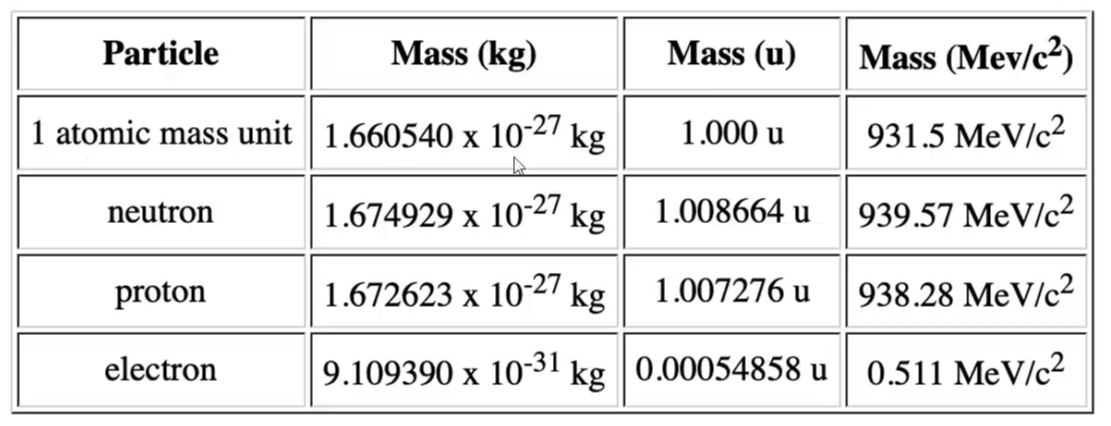
\includegraphics[width = \textwidth]{nucleon_mass_table.png}
    \caption{Table of the masses of the nucleons. $c^2 = 931.5$MeV/u. In reality, the mass of the proton is slightly less than the mass of the neutron. The proton is 2000 times more massive than the electron.}
    \label{fig: }
\end{figure}


\section{Nuclear Properties}
The parameters which describe the nucleus are. There are two types of nuclear properties: static and dynamic.
\begin{itemize}
    \item Static: Charge, Radius, mass, Binding energy, Angular momentum, Parity, Magnetic dipole moment, Electric quadrupole moments, Exited states and their energies. 
    \item Dynamic: Shape, Decay
\end{itemize}

\subsection{Connected Terms}
\begin{itemize}
    \item Charge/Charge Distribution: Protons. Found via electron scattering \cref{subsec: Nuclear Charge Distribution from Electron Scattering} by the Coulomb interaction. 
    \item Matter/Mass Distribution: Nucleons. Found via hadron scattering \cref{subsec: Nuclear Mass Distribution from Hadron Scattering}, alpha particles (Rutherford), protons and neutrons by using the strong force.
    \item Radius: Size of the nucleus (nucleons)
\end{itemize}

\subsection{Charge Distribution}
To probe the charge distribution of the nucleus, we use charged particles. We also need the following:
\begin{itemize}
    \item A beam of charged particles (often protons)
    \item Wavelength should be similar or smaller than the nucleus (about 10fm in diameter). 
    \item Electrons were popular in the 50's. 
    \item An energy of 100 Mev to 1 GeV is needed.
    \item Calculating the energy needed is done by using the de Broglie wavelength where $λ = h / p$ with $λ ≤ 10$fm. 
\end{itemize}

\subsection{Nuclear Charge Distribution from Electron Scattering}\label{subsec: Nuclear Charge Distribution from Electron Scattering}
\begin{itemize}
    \item Radius increases with mass number $A$
    \item The central nuclear charge density is nea4rly the same for all nuclei. Nucleons do not seem to concentrate near the center of the nucleus, but instead have a constant distribution along the surface. 
    \item The number of nucleons per unit volume is roughly constant:
    \begin{equation}
    \frac{A}{\frac{4}{3}πR^3} ≈ \text{const}
    \end{equation} 
    \item The radius of the nucleus is proportional to $A^{1/3}$. 
    \begin{equation}
    R = R_0A^{1/3} \quad , \quad  R_0 ≈ 1.2 \text{ fm}
    \end{equation}
\end{itemize}

\subsection{Nuclear Size}
We can find the radius of a nucleus by using the scattering angle of the local minimum of the Rutherford cross-section, see \cref{fig: electron_scattering_angles}. The diffraction pattern is not exactly that of a circular disk, as the nucleus does not have a well-defined surface.
\begin{figure}[ht!]
\centering
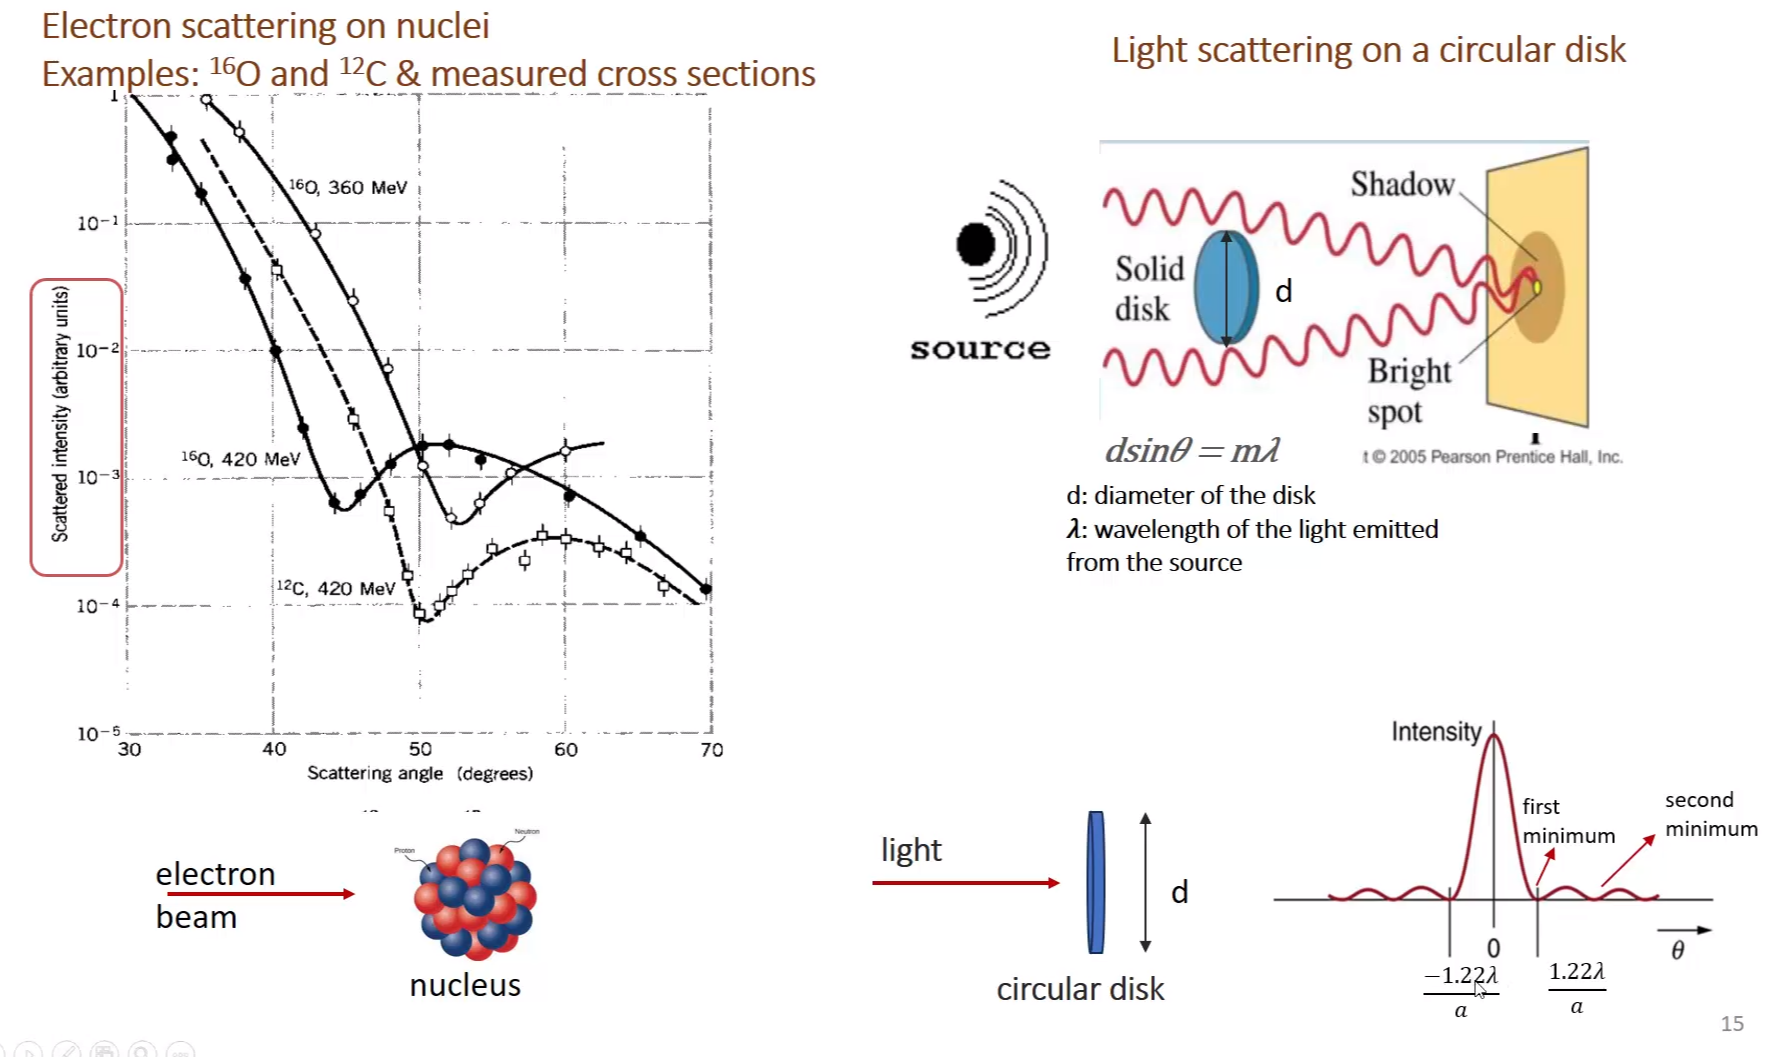
\includegraphics[width = \textwidth]{electron_scattering_angles.png}
\caption{Example of the local minimum of the Rutherford cross-section. The angle is used to calculate the radius of the nucleus.}
\label{fig: electron_scattering_angles}
\end{figure}
\begin{equation}
\sin θ = \frac{1.22λ}{d} ⇒ R = \frac{d}{2} = \frac{1.22λ}{2\sin θ}
\end{equation}
This is only a rough estimate as the angle is calculated in two dimensions, instead of three. 


\subsection{Nuclear Mass Distribution from Hadron Scattering}\label{subsec: Nuclear Mass Distribution from Hadron Scattering}
\begin{itemize}
    \item Electrons only mostly interact with protons. We therefore use hadrons to study the mass distribution of the nucleus.
    \item The radius is proportional to the nuclear rather than the Coulomb force. 
    \item The Rutherford experiment showed that the nucleus is a point-like object.
\end{itemize}

\subsubsection{Fixed Angle of Observation with Changing Energy}
\begin{itemize}
    \item At low energies the alpha particles and the $^{208}$Pb nucleus interact with the Coulomb interacting as with Rutherford scattering.
    \item With increasing energy, the repulsion from the Coulomb force is overcome, and the strong force becomes the dominant force. The Rutherford formula no longer holds. 
    \item The alpha particles became absorbed by the nucleus and only a small fraction is scattered. 
    \item When energy is high enough, we get the diffraction pattern.
\end{itemize}

\subsection{Conclusion from Charge Radius Experiments}
\begin{itemize}
    \item The charge and mass radii of nuclei is nearly equal to within about $0.1$fm. 
    \item Both show the same $A^{1/3}$ dependence with $R_0 = 1.2$fm. 
    \item As heavy nuclei have about 50 \% more neutrons than protons, we might expect the neutron distribution to be more extended than the proton distribution. This is not the case as the neutrons pulls inwards, and the protons push outwards, until they are mixed such that the radius is the same. 
\end{itemize}



\subsection{Nuclear Mass}
\subsection{Deflection Spectrometer}
\begin{figure}[ht!]
\centering
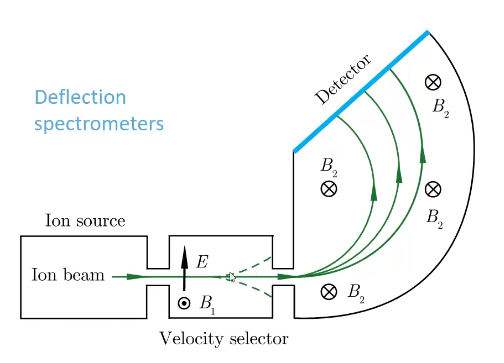
\includegraphics[width = .5\textwidth]{deflection_spectrometer.png}
\caption{Experimental setup for measuring the mass of a particle.}
\label{fig: deflection_spectrometer}
\end{figure}

\begin{itemize}
    \item Shooting a ray of charge particles affected by a magnetic field and measuring the deflection we can calculate its mass. 
    \item To measure an entire particle they must be ionized. The electrons carry so little mass that they are neglected.
    \item After ionization, the particles travel through an electric and magnetic field. 
    \item Only the particles with the right velocity will pass through the fields and be subjected to the new magnetic field. 
    \item The new field will deflect the particles according to their $m / q$ value. 
\end{itemize}
\subsubsection{Calculating the Mass}
\begin{equation}
F_{B} = q \vec{v} × \vec{B} 
\end{equation}
The field and velocity are perpendicular.
\begin{equation}
F_{B} = qvB
\end{equation}
\begin{equation}
F_E = F_B ⇒ qE = qvB ⇒ v = \frac{E}{B_1}
\end{equation}
$B_1$ is the first magnetic field as seen in \cref{fig: deflection_spectrometer}. The force from the magnetic field centripetal force. 
\begin{equation}
F_B = \frac{mv^2}{r} = qvB_2
\end{equation}
\begin{equation}
\frac{mv}{r} = qB_2
\end{equation}
\begin{equation}  
\frac{m}{q} = \frac{B_2ρ}{v}
\end{equation}
The radius of the circle is given by $r = ρ$. Setting $B_1 = B_2$ gives the following for the mass.
\begin{equation}
m = \frac{B_1 B_2 ρ}{E} = \frac{B^2 ρq}{E}
\end{equation}
where $q$ is the charge of the particle.

\paragraph{Accuracy}
\begin{itemize}
    \item These measurements are very important for mass models used in other parts of physics. 
    \item The accuracy is about $Δm / m = 10^{6-}$, but that is not enough. 
    \item The mass doublet technique gives a precision of $10^{-8}$ / $10^{-9}$
\end{itemize}






 %#  2
\section{Binding Energy}
\subsection{Formulas and Definitions}
\begin{itemize}
    \item Binding Energy: The energy required to keep the nucleus together. The mass of the nucleus is not equal to the sum of its parts. The mass of the individual nucleons is higher than the mass of the nucleus. The difference is the binding energy.
    \begin{equation}
    Zm_p + Nm_n - M_{\text{Nucleus}} = \text{Binding Energy}  \quad ⇒ \quad Zm_p + Nm_n > M_{\text{Nucleus}}
    \end{equation}
\end{itemize}

\subsection{Mass of the Nucleus}
The total mass of the atom is the mass of the nucleus and electrons, minus the binding energy of the electrons. 
\begin{equation}
M_{\text{Atom}} = M_{\text{Nucleus}} + Zm_e - \underbrace{∑_{i=1}^{Z} B_i / c^2}_{\text{Often negligible}}
\end{equation}

\begin{equation}
M_{\text{Atom}} = M_{\text{Nucleus}} + Zm_e
\end{equation}

$M$ usually refers to the mass of the entire atom, and so the subscript "Atom" is often omitted. We usually write the atom using the following notation:
\begin{equation}
M\left(_{Z}^{A}X_{N}\right) = M_{\text{Nucleus}} \left(_{Z}^{A}X_{N}\right) + Zm_e
\end{equation}
Multiplying by $c^2$ we get the mass in energy units ($E = mc^2$):
\begin{equation}
M_{\text{Nucleus}}\left(_{Z}^{A}X_{N}\right) = M\left(_{Z}^{A}X_{N}\right) - Zm_ec^2
\end{equation}
\begin{equation}
\underline{\underline{M_{\text{Nucleus}}\left(_{Z}^{A}X_{N}\right)c^2 = M\left(_{Z}^{A}X_{N}\right)c^2 - Zm_e c^2 
}}
\end{equation}
\subsection{Nuclear Binding Energy (B.E.)}
This energy is very small compared to the mass energy of the nucleus. We can derive this from the mass of the nucleus. 
\begin{align}
    B.E. &= \left(Zm_{p} + Nm_{n} - M_{N}\left(_{Z}^{A}X_{N}\right)\right) c^2 \\
    &= \left(Zm_{p} + Nm_{n} - \left(M\left(_{Z}^{A}X_{N}\right) - Zm_e\right)\right) c^2 \\ 
    &= \left(Z(\underbrace{m_{p} + m_e}_{\text{Hydrogen}}) + Nm_{n} - M\left(_{Z}^{A}X_{N}\right)\right) c^2 \\ \\
   B.E. &= \underline{\underline{\left(Zm\left(^{1}H\right) + Nm_{n} - M\left(_{Z}^{A}X_{N}\right)\right) c^2}}
\end{align}
As the units so far has been energy $(mc^2)$ we can switch to MeV. 
\begin{equation}
B.E. = \left[mc^2\right] = \left[uc^2\right] = u931.5\text{MeV /}u \quad ⇒ \quad c^2 = 931.5 \text{MeV/u}
\end{equation}
\begin{equation}\label{eq: binding_energy}
B.E. = \underline{\underline{\left(Zm\left(^{1}H\right) + Nm_{n} - M\left(_{Z}^{A}X_{N}\right)\right) 931.5 \text{MeV/u}}}
\end{equation}

\subsubsection\protect{Example: Helium $_{2}^{4}H_{2}$}
We use the formula for binding energy from \cref{eq: binding_energy} to calculate the binding energy of the hydrogen atom $_{2}^{4}He_{2}$.
\begin{align}
B.E. &= \left(2m_p + 2m_n - M\left(_{2}^{4}He_{2}\right)\right) 931.5 \text{MeV/u} \\
&= \left(2 ⋅ 1.007825u + 2 ⋅ 1.008664u - 4.002603u\right) ⋅ 931.5 \text{MeV/u} \\
&= \underline{\underline{0.0304 ⋅  931.5 \text{ MeV} = 28.3 \text{ MeV}}}\label{eq: helium_binding_energy}
\end{align}
The ratio between the binding energy and the rest mass of the nucleus is very small. Using the binding energy from \cref{eq: helium_binding_energy} and the mass of the helium nucleus, we can calculate the ratio:
\begin{equation}
\frac{28.3}{3728} = 0.75\%
\end{equation}
\subsection{Nuclear Separation Energy}
The energy required to separate a proton $S_{p}$ or a neutron $S_{n}$ from the nucleus.
\subsubsection{Neutron Separation Energy}\label{sssec: neutron_separation_energy}
It requires lower energy to remove a neutron from a nucleus with an odd number of neutrons. This is because one is unpaired. 
\begin{equation}
S_n = \left(M\left(_{Z}^{A-1}X_{N-1}\right) - M(_{Z}^{A}X_{N} + m_n)\right)c^2
\end{equation}
This can also be expressed using binding energies as mass and energy are equivalent through $E = mc^2$:
\begin{equation}
S_n = B\left(_{Z}^{A}X_{N}\right) - B\left(_{Z}^{A-1}X_{N-1}\right)
\end{equation}

\subsubsection{Proton Separation Energy}
Using the same logic as for the neutron separation energy \cref{sssec: neutron_separation_energy}, we can express the proton separation energy through the binding energies. It's important to keep in mind that after loosing a proton, the element changes.
\begin{equation}
S_p= \left(M\left(_{Z-1}^{A-1}Y_{N}\right) - M(_{Z}^{A}X_{N} + \underbrace{m_p + m_n}_{_{1}^{1}H_{}})\right)c^2
\end{equation}
\begin{equation}
S_p = B\left(_{Z}^{A}X_{N}\right) - B\left(_{Z-1}^{A-1}Y_{N}\right)
\end{equation}

% \subsection{Average Binding Energy}
\begin{itemize}
    \item Except for very light nuclei, the binding energy per nucleon is linear. It's almost constant at around 8 MeV/nucleon.
    \item The highest binding energy per nucleon is around $A = 60$ with the highest binding energy per nucleon at $^{56}\text{Fe}$. 
    \item When going from heavier elements towards iron we get nuclear fission
    \item When going from lighter elements towards iron we get nuclear fusion
\end{itemize}

\begin{figure}[h!]
\centering
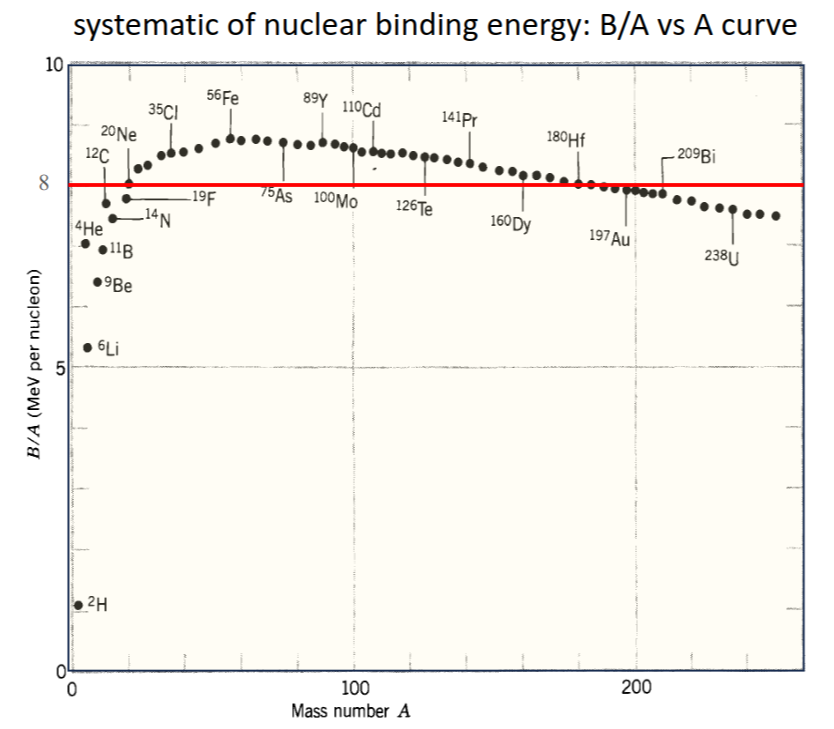
\includegraphics[width = .75\textwidth]{BE_per_nucleon.png}
\caption{}
\label{fig: BE_per_nucleon}
\end{figure}

\subsection{Semi-Empirical Mass Formula}
\begin{itemize}
    \item Sets out to explain the binding energies of nuclei.
    \item It is semi-empirical as the five of its constant are found by experiment.
    \item Tries to recreate the binding energy per nucleus graph in \cref{fig: BE_per_nucleon} by using the \textit{liquid drop model}.
\end{itemize}

\begin{equation}\label{eq: semi_empirical_mass_formula}
B = a_vA - a_sA^{2 / 3} - a_c\frac{Z(Z-1)}{A^{1 / 3}} - a_{\text{asym}}\frac{(A-2Z)^2}{A} + δ
\end{equation}
\subsubsection{Explanation of the Terms in the Semi-Empirical Mass Formula}\label{sssec: Explenation of the Terms in the Semi-Empirical Mass Formula}
\begin{itemize}
    \item $\mathbf{a_vA}$: \textbf{Volume term}. The binding energy is proportional to the volume of the nucleus approximated to a sphere $\left(V = 4πR^3/3\right)$. This dominates the binding energy for large nuclei. 
    \begin{equation}
    a_v ≈ 15.8 \text{ MeV}
    \end{equation}
    The linear dependence of the binding energy on the number of nucleons tells us that the strong force is short range as each nucleon only interacts with its nearest neighbors. 
    \item $\mathbf{a_sA^{2 / 3}}$: \textbf{Surface term}. The volume term is not quite accurate as the nucleons on the surface have fewer neighbors. This term corrects for that. The binding energy is proportional to $πR^2$
    \begin{equation}
    a_s ≈ 16.8 \text{ MeV}
    \end{equation} 
    \item $\mathbf{a_cZ(Z-1)A^{-1 / 3}}$: \textbf{Coulomb term}. The binding energy is reduced by the repulsion between the protons. It is therefore detracted. The Coulomb force is long range and is therefore proportional to $Z(Z-1)$ as all protons interact. 
    \begin{equation}
    a_c ≈ 0.72 \text{ MeV}
    \end{equation}
    \item $\mathbf{a_{\text{asym}}(A-2Z)^2A^{-1}}$: \textbf{Asymmetry term}. Stable nuclei have a balance between protons and neutrons. As the ratio of protons to neutrons deviate from 1, the nuclei becomes less stable (lower binding energy). This inhibits Hydrogen or Helium atoms with many neutrons. It is caused by the Pauli exclusion principle as nucleons are fermions and therefore can not occupy the same state at once. 
    \begin{equation}
    a_{\text{asym}} ≈ 23 \text{ MeV}
    \end{equation}
    Heavier nuclei must have more neutrons to fight the Coulomb repulsion. The term gets relatively small as the number of nucleons increases. 
    \item $\mathbf{δ}$: \textbf{Pairing term}. This term is not included in the original formula, but is added to account for the fact that nuclei with an even number of protons and neutrons are more stable. This is because the nucleons in the same space-state can be coupled to have a total spin of 0. They are therefore closer together and therefore more tightly bound with a higher binding energy. This is called even-even nuclei. 
    \begin{equation}
    δ =  \begin{cases}
        +a_pS^{-3 / 4}, &\text{ if even(N)-even(Z)}\\
        0, &\text{ if odd(A)}\\
        -a_pS^{-3 / 4}, &\text{ if odd(N)-odd(Z)}\\
    \end{cases} 
    \end{equation}
    \begin{equation}
    a_p ≈ 34 \text{ MeV}
    \end{equation}
\end{itemize}
\subsubsection{SEMF Conclusion}
\begin{itemize}
    \item The semi-empirical mass formula was a first attempt at understanding how binding energy works. 
    \item It is semi-empirical as the constants are found by experiment. 
    \item A negative binding energy means the nucleus is not bound and is therefore not stable.
\end{itemize}
\begin{equation}
B = \underbrace{a_vA - a_sA^{2 / 3} - a_cZ(Z-1)A^{-1 / 3}}_{\text{Liquid-drop model for energy calculations}} - \underbrace{a_{\text{asym}}(A-2Z)^2A^{-1} + δ}_{\text{Interactions between nucleons}}
\end{equation}
\begin{figure}[h!]
\centering
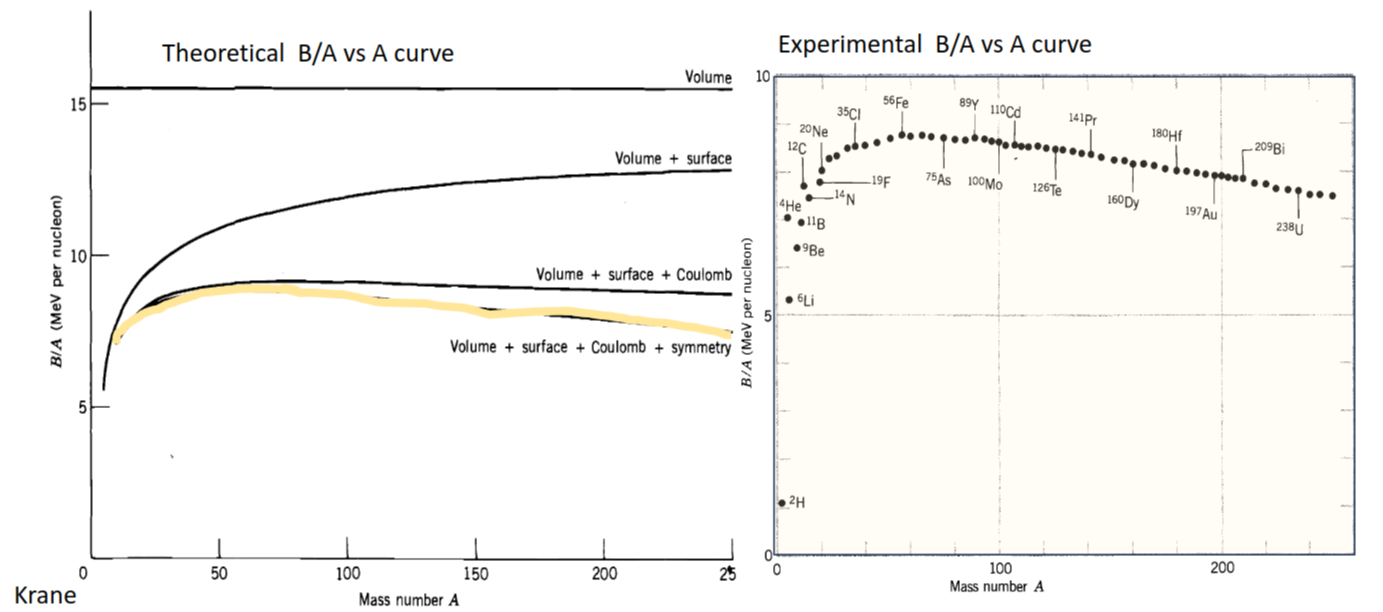
\includegraphics[width = \textwidth]{SEMF_term_addition.png}
\caption{Plot of how the different terms in the semi-empirical mass formula \cref{eq: semi_empirical_mass_formula} gets us closer to the experimental values}
\label{fig: SEMF_term_addition}
\end{figure}



 %#  3
\subsection{Mass Parabolas of Isobars}
Isobars have the same number of nucleons (A).
\begin{align}
M(A,Z) &= Z(\overbrace{m_p + m_e}^{M(_{}^{1}H_{})}) + (\underbrace{A-Z}_{\text{neut. num.}})m_n - B(A,Z) /c^2 \\
B(A,Z) &= a_vA - a_sA^{2 / 3} - a_c\frac{Z(Z-1)}{A^{1 / 3}} - a_a\frac{(A-2Z)^2}{A} + \delta(A,Z)
\end{align}
\subsubsection{Finding the Minimum of the Mass Parabola}
As the parabola is mass $M$ as a function of $Z$, we can find the minimum by taking the derivative with respect to $Z$ and setting it equal to zero.
\begin{align}
\frac{∂ M}{∂ Z} &= 0 \\
Z_{\text{min}} &= \frac{(m_n - m_p - m_e)+a_cA^{-1 / 3} + 4a_{\text{sym}}}{2a_{c} A^{-1 / 3} + 8a_{\text{sym}}A^{-1}}
\end{align}
We can approximate this as the following:
\begin{equation}
Z_{\text{min}} ≈ \frac{A}{2} - \frac{1}{1 + \frac{1}{4}A^{2/3}a_c / a_{\text{sym}}} \quad , \quad  a_{\text{sym}} ≈ 23 \text{ MeV} \ , \ a_c ≈ 0.72 \text{ MeV}
\end{equation}

\paragraph{Example: A = 10}
This is stable for smaller nuclei. 
\begin{equation}
Z_{\text{min}} ≈ 5 \quad \text{ and } \quad  \frac{Z_{\text{min}}}{A} ≈ 0.5
\end{equation}

\paragraph{Example: A = 200}
A lower ratio is stable for larger nuclei.
\begin{equation}
Z_{\text{min}} ≈ 79 \quad \text{ and } \quad  \frac{Z_{\text{min}}}{A} ≈ 0.4
\end{equation}

\subsubsection{Valley of (beta) stability}
\begin{itemize}
    \item As can be seen in \cref{fig: valley_beta_stability}, we have two parabolas for $A = 128$ as it can be odd-odd or even-even. Higher binding energy is more stable.
    \item The even-even isobar is more stable as explained in \cref{sssec: Explenation of the Terms in the Semi-Empirical Mass Formula}, because the nucleons can pair up in the same space-state with opposite spins and therefore be closer to each other and thus more stable.
    \item Only the atom in the bottom of the valley is stable. The others are prompt to beta decay downwards. 
    \item Double beta decay can happen with even numbers of nucleons as can be seen for $A = 128$ with $Z = 52$, as $Z = 53$ has higher energy, and it is therefore forced to decay all the way up to $Z = 54$. 
\end{itemize}
\begin{figure}[h!]
\centering
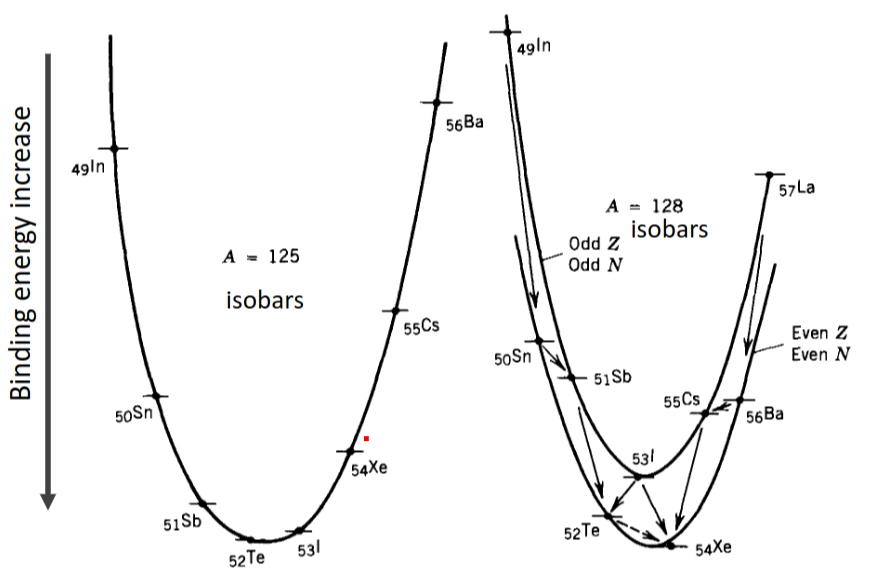
\includegraphics[width = .6\textwidth]{valley_beta_stability.png}
\caption{Valley of (beta) stability for different isobars with $A = 125$ and $A = 128$. The higher the binding energy, the more stable the isobar.}
\label{fig: valley_beta_stability}
\end{figure}

\paragraph{Beta Decay}
\begin{itemize}
    \item $β+$: Proton rich nuclei decay by converting a proton into a neutron, a positron and a neutrino. 
    \item $β-$: Neutron rich nuclei decay by converting a neutron into a proton, an electron and an antineutrino.
\end{itemize}
\begin{figure}[h!]
\centering
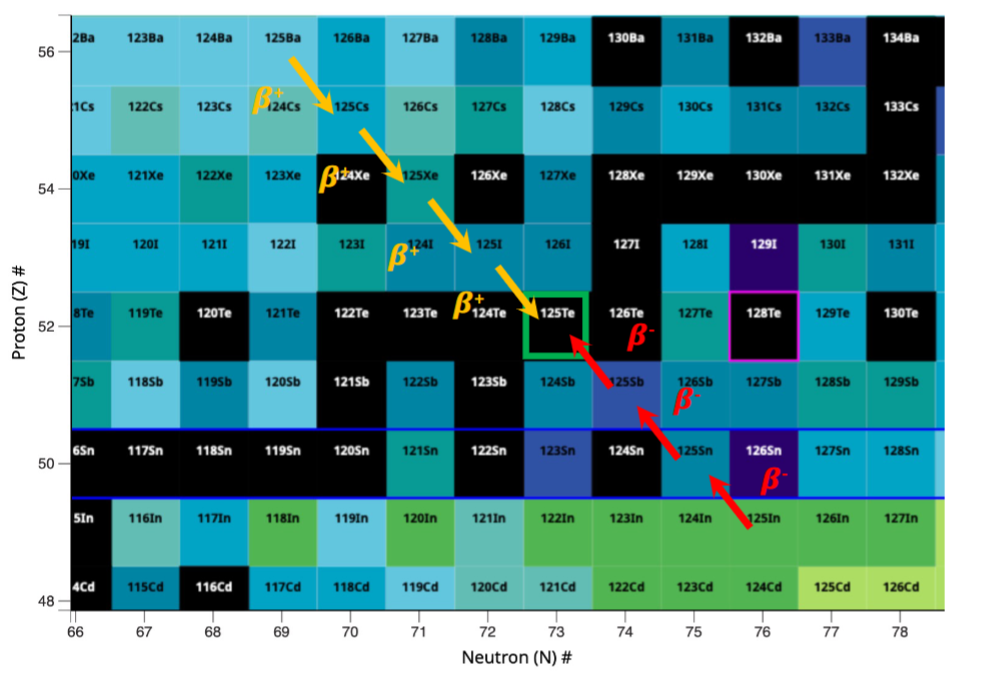
\includegraphics[width = \textwidth]{bet_decay_chart.png}
\caption{Chart showing different elements and their decays.}
\label{fig: bet_decay_chart}
\end{figure}


 %#  4
\section{Angular Momentum \& Parity}
\subsection{Angular Momentum of the Nucleus}
\begin{itemize}
    \item Total angular momentum $j = l + s$ is the sum of the orbital angular momentum $l$ and the spin $s$. 
    \item Both $l$ and $s$ are quantized, and the total angular momentum $j$ is also quantized.
    \item Nucleons are fermions and therefore spin half particles. 
    \item Fermions can't rotate, but still have spin $s$. There is no classical analogy for this. $l$ is the orbital angular momentum and is just like the classical angular momentum.
\end{itemize}
\subsubsection{Orbital Angular Momentum}
Angular momentum is a vector and thus has both magnitude and direction. As the values are quantized we use the quantum numbers $l$, $s$ and $j$ to describe the magnitude and direction. 
\begin{itemize}
    \item $l$ is the orbital angular momentum and can take the values $0, 1, 2, 3, \ldots$.
    \item Magnitude: 
    \begin{align}
    l &= \sqrt{l(l+1)}ℏ \\
    l_z &= m_lℏ \quad , \quad m_l ∈ \{-l, -l+1, \ldots, l-1, l\} 
    \end{align} 
    \item Direction \cref{fig: angular_momentum_sphere}:
    \begin{figure}[h!]
        \centering
        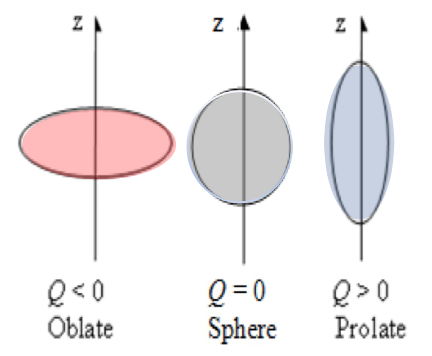
\includegraphics[width = .75\textwidth]{angular_momentum_sphere.png}
        \caption{Orbital angular momentum vector visualized on a sphere.}
        \label{fig: angular_momentum_sphere}
    \end{figure}
\end{itemize}    

\subsubsection{Spin}
\begin{itemize}
    \item Spin is a property of particles and is not related to the motion of the particle. 
    \item Spin is quantized and can take the values $s = \frac{1}{2}$ or $s = -\frac{1}{2}$.
    \item Magnitude: 
    \begin{align}
    s &= \sqrt{s(s+1)}ℏ \\
    s_z &= m_sℏ \quad , \quad m_s ∈ \{-s, -s+1, \ldots, s-1, s\} 
    \end{align} 
    \item As the spin $s$ can only be $1 / 2$, the magnetic quantum number $m_s$ can only be $\pm 1 / 2$
    \item Direction \cref{fig: spin_direction}: There is no classical analogy for direction, but if in a magnetic field, the spin will align with or against the field 
    \begin{figure}[h!]
    \centering
    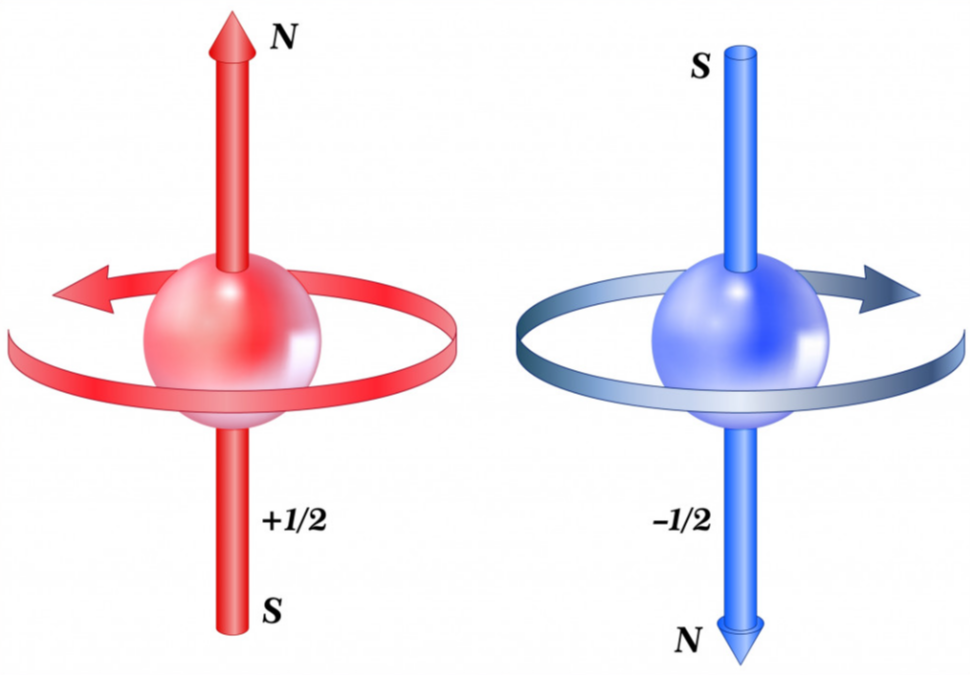
\includegraphics[width = .75\textwidth]{spin_direction.png}
    \caption{Visual representation of the spin of a nucleon in a magnetic field.}
    \label{fig: spin_direction}
    \end{figure}
\end{itemize}
\newpage
\subsubsection{Total Angular Momentum}
\begin{itemize}
    \item The total angular momentum $j$ is the sum of the orbital angular momentum $l$ and the spin $s$.
    \item Magnitude: 
    \begin{align}
    j &= \sqrt{j(j+1)}ℏ \\
    j_z &= m_jℏ \quad , \quad m_j ∈ \{-j, -j+1, \ldots, j-1, j\} \\
    m_j &= m_l + m_s = m_l ± \frac{1}{2}
    \end{align}
    \item Direction \cref{fig: total_angular_momentum_visualized}:
    \begin{figure}[h!]
    \centering
    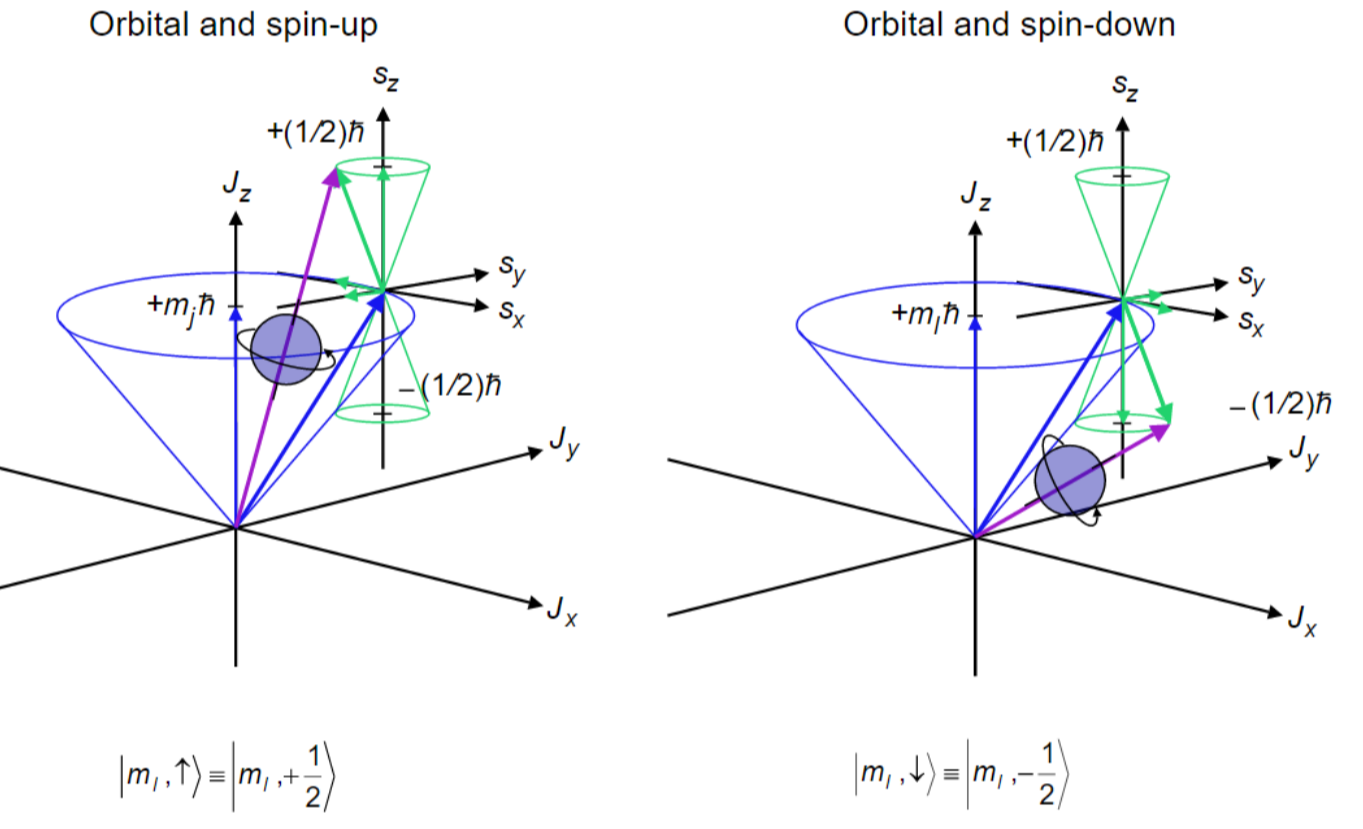
\includegraphics[width = .75\textwidth]{total_angular_momentum_visualized.png}
    \caption{Total angular momentum visualized in 3D.}
    \label{fig: total_angular_momentum_visualized}
    \end{figure}
\end{itemize}

\subsubsection{Total Angular Momentum of the Nucleus}
\begin{itemize}
    \item The sum of the angular momentum of all the nucleons in the nucleus. 
    \begin{align}
    \vec{I} &= \sum_{i=1}^{A} \vec{j}_i \quad , \quad  \vec{j}_i = \vec{l}_i + \vec{s}_i \\
    I &= \sqrt{I(I+1)}ℏ \\
    I_z &= mℏ \quad , \quad m ∈ \{-I, -I+1, \ldots, I-1, I\}
    \end{align} 
    \item As each nucleus has half-integer total angular momentum, odd number of nucleons $A$ will have half-integer total angular momentum, and even number of nucleons will have integer total angular momentum.
    \item All the known even-even nuclei have spin-0 ground states. 
    \item As a result, the ground state of an odd $A$ nucleus must be the $j$-value of the odd proton or neutron. 
\end{itemize}

\subsection{Parity}
Parity is the behavior of a system under the inversion of all spatial coordinates $\vec{r} → - \vec{r}$
\begin{itemize}
    \item Cartesian coordinates: $r → (-x, -y, -z)$. 
    \item Spherical coordinates: $r → (r, π-θ, φ + π)$.
    \item The parity operator is $\hat{P}$ and has two effects on the wave function: 
    \begin{itemize}
        \item Even parity (+): $\hat{P}ψ(\vec{r}) = ψ(\vec{r})$.
        \item Odd parity (-): $\hat{P}ψ(\vec{r}) = -ψ(\vec{r})$.
        \item An even function is symmetric around the origin and an odd function is antisymmetric around the origin. This means $ψ(-r) = ψ(r)$ or $ψ(-r) = -ψ(r)$. 
        \item Visual representation \cref{fig: even_vs_odd_function}:
        \begin{figure}[h!]
        \centering
        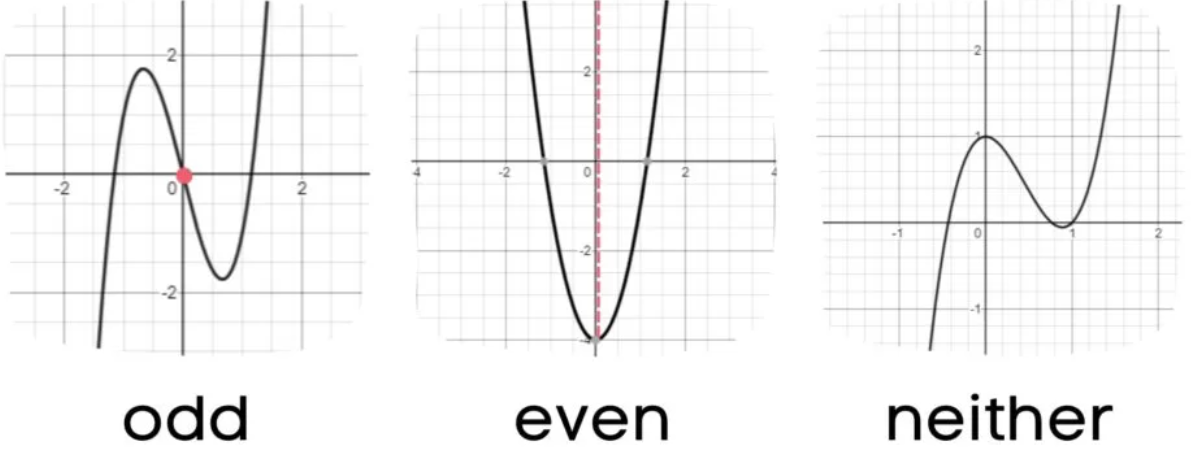
\includegraphics[width = .75\textwidth]{even_vs_odd_function.png}
        \caption{Visual representation of even and odd functions.}
        \label{fig: even_vs_odd_function}
        \end{figure}
    \end{itemize} 
\end{itemize}
\subsubsection{Splitting the Wave Function}
\begin{itemize}
    \item The wave function can be split into its radial and angular parts.
    \begin{align}
    Ψ(\vec{r}) &= R(r)Y(\theta, φ) \\
    \hat{P}R(r) &= R(r) \\
    \hat{P}Y(\theta, φ) &= (-1)^lY_{l}^{m}(θ, ϕ)
    \end{align} 
    \item Parity of state with orbital angular momentum $l$ 
    \begin{equation}
    π(-1)^{l}
    \end{equation} 
    \item By convention, the intrinsic parity of the nucleon is $π = +1$, because they are fermions. Anti-fermions (like positron) have $π = -1$.
    \item For a composite system, the parity is the product of the intrinsic parities of the constituents.
    \begin{equation}
      π_{\text{total}} = (-1)^{L}π_1π_2π_3 \ldots \quad , \quad  L = l_1 + l_2 + l_3 + \ldots
    \end{equation}
\end{itemize}

\section{Electric and Magnetic Moments}
\begin{itemize}
    \item The protons create a magnetic and electric fields. 
    \item A distribution of charge is assigned an electric dipole moment of either monopole, dipole, quadrupole, octopole, etc.
    \item A spherical charge distribution gives only a monopole. 
    \item A circular current only gives a magnetic dipole. 
    \item Nuclei tend to have as simple of dipole moments as possible. 
    \begin{itemize}
        \item L = 0: Monopole
        \item L = 1: Dipole
        \item L = 2: Quadrupole
        \item L = 3: Octopole
    \end{itemize}
\end{itemize}

\subsection{Parity Selection Rules}
\subsubsection{Electric Dipole Moments $E_0$}
\begin{equation}
  L = 0, 2
\end{equation}
Allowed values are $L ∈ {0,2}$ with a parity of $(-1)^{L}$. A dipole is a measure of the separation of positive and negative charge. In the nucleus there is no separation. 

The electric monopole moment is just the charge of the nucleus $Z ⋅ e$.


\subsubsection{Magnetic Dipole Moments $M_1$}
\begin{equation}
  L = 1
\end{equation}
Allowed values are $L = 1$ with a parity of $(-1)^{L+1} = 1$. The magnetic monopole has not been observed. 

As the charged particles are moving, they create a magnetic field. For an electron orbiting a nucleus, we get the following:
\begin{equation}
  \left|\vec{μ}\right| = \frac{e}{2πr / v} πr^2 = \frac{e}{2m}\left|\vec{l}\right|
\end{equation}
This connects the magnetic moment to the mass of the particle. The same goes for the protons in the nucleus. We know the $z$-component of the orbital angular momentum and can be inserted to the equation:
\begin{equation}
  μ = \frac{eℏ}{2m}l
\end{equation}
\subsection{Bohr Magneton \& Nuclear Magneton}
For atomic motion, the electron mass is used.
\begin{align}
μ_{B} = \frac{eℏ}{2m_{e}}  = 5.788 ⋅ 10^{-5} \text{ eV/T}
\end{align}
For nuclear motion, the proton mass is used.
\begin{align}
μ_{N} = \frac{eℏ}{2m_{p}}  = 3.152 ⋅ 10^{-8} \text{ eV/T}
\end{align}

As $μ_{B} ≫ μ_{N}$, the nuclear magnetic moment plays much smaller role in atomic physics.

\subsection{Magnetic Moments of Nuclei}
\begin{itemize}
    \item Magnetic Dipole Moment:
    \begin{itemize}
        \item The magnetic dipole moment of the nucleons is caused by their orbital motion. $μ = g_l μ_{N}l$. 
        \item The g-factor $g_l$ is a dimensionless quantity characterizing the magnetic moment of the atom, nucleus or other particle in question. 
        \item Protons have $g_l = 1$
        \item Neutrons have $g_l = -0.5$. It was believed to be zero, but it proves it's not a point particle.
    \end{itemize}
    \item Spin Magnetic Dipole Moment:
    \begin{itemize}
        \item The magnetic dipole moment of the nucleons is caused by their spin. $μ = g_s μ_{N}s$.
        \item The g-factor $g_s$ is a dimensionless quantity characterizing the magnetic moment of the atom, nucleus or other particle in question.
        \item Protons have $g_s = 5.59 ± 0.0000022$
        \item Neutrons have $g_s = -3.82 ± 0.0000022$. This is unexpected as the neutron is a neutral particle. This shows there charge inside the neutron, and it is not a point particle.
        \item Electrons have $g_s = 2$
    \end{itemize}
\end{itemize}

\subsubsection{Nuclear Structure from Magnetic Moments}
\begin{itemize}
    \item The pairing force favors the coupling of the nucleons such that the sum of their total angular momentum is zero. 
    \item As a result, the magnetic moment of the nucleus is determined by the unpaired nucleons.
    \item Example \cref{fig: nuclear_magnetic_dipole_samples}:
    \begin{figure}[h!]
    \centering
    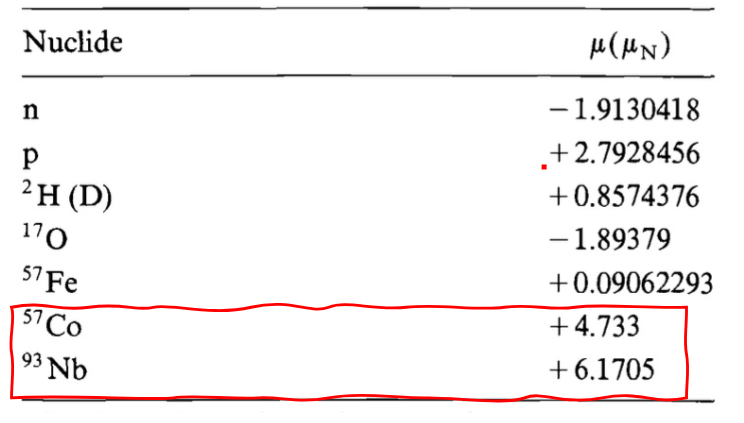
\includegraphics[width = .75\textwidth]{nuclear_magnetic_dipole_samples.png}
    \caption{Table showing the magnetic dipole moments of different nuclei. The box in red shows how larger atoms have a larger magnetic dipole moment, caused by more unpaired nucleons.}
    \label{fig: nuclear_magnetic_dipole_samples}
    \end{figure}
    
\end{itemize}

\subsection{Electric Quadrupole Moments $E_2$ \& Shape of the Nucleus}
Visual representation of the electric quadrupole moments effect on the shape of the nucleus in \cref{fig: nucleus_shape_E2}. 
\begin{equation}
  eQ = e ∫ ψ^{*}(3z^2 - r^2)ψ \ \mathrm{d}v
\end{equation}
Experiment shows that large nuclei like Barium, has a pear-like shape. 
\begin{figure}[h!]
\centering
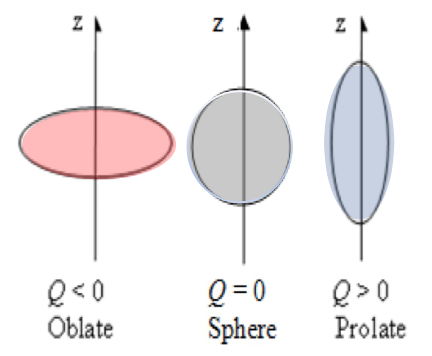
\includegraphics[width = .5\textwidth]{nucleus_shape_E2.png}
\caption{Shape of the nucleus as a function of the electric quadrupole moment.}
\label{fig: nucleus_shape_E2}
\end{figure}

 %#  5
\subsection{Example: Calculating Parity of State}
\paragraph{Case 1: Calculate the parity of two nucleons in the $p_{3 /2}$ orbital} 
In the $p_{3 /2}$ orbital, we know $l = 1$. As all nucleons are fermions, the parity $π$ of the orbital is $(-1)^l = -1$.
\paragraph{Case 2: Calculate the parity of two nucleons in the $g_{9 /2}$ orbital}
In the $g_{9 /2}$ orbital, we know $l = 4$. As all nucleons are fermions, the parity $π$ of the orbital is $(-1)^l = 1$.

\subsection{Level Schemes \& Excited States}
\begin{itemize}
    \item Some nuclei have more excited states than others. This is regularly associated with even-$Z$ and even-$N$ nuclei in the interval $150 ≤ A ≤ 190$. 
    \item Comparing the level schemes of different nuclei : 
    \begin{figure}[h!]
    \centering
    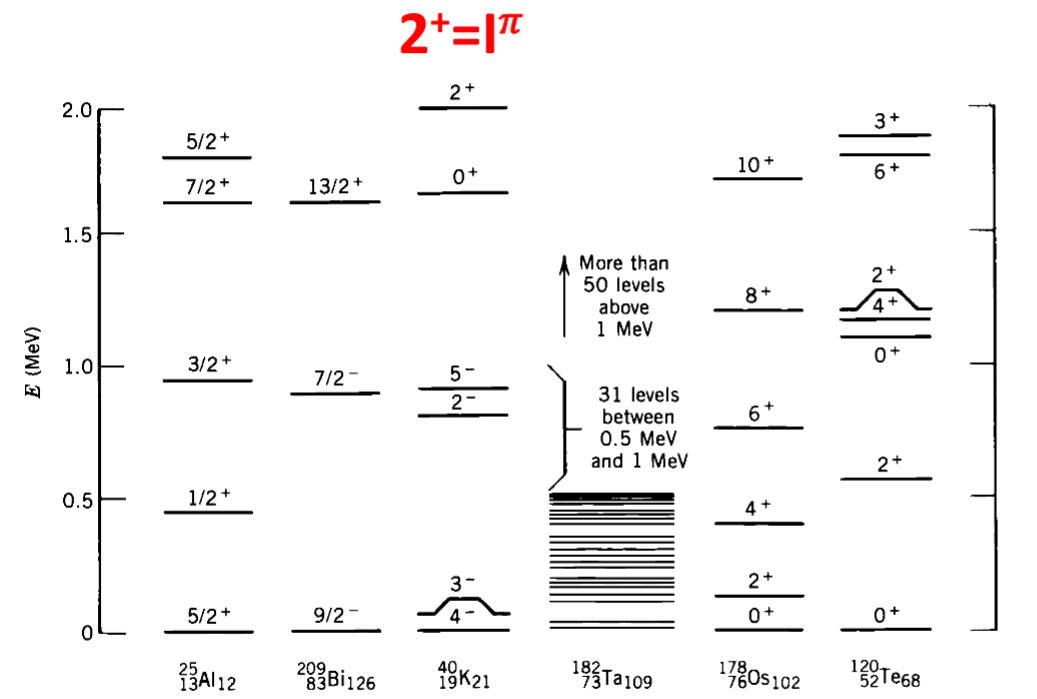
\includegraphics[width = .75\textwidth]{nuclei_excitation_levels_comparison.png}
    \caption{Some nuclei have more complex level schemes than others}
    \label{fig: nuclei_excitation_levels_comparison}
    \end{figure}
    
\end{itemize}


\section{Nuclear Force}
\begin{itemize}
    \item The strong force is very attractive at short distances. Even stronger than the Coulomb force. 
    \item Negligible at greater distances than 1-2 fm. 
    \item Some particles are immune, such as electrons. Electrons are 100,000 fm away from the nucleus.  
    \item The strong force becomes very repelling at distances smaller than 1 fm. 
    \item Nuclear force is nearly charge independent. We know this from experiments on excited states of \textit{mirror nuclei} (same $A$, but opposite $N$ and $Z$) as seen in \cref{fig: mirror_nuclei_excitation_levels_comparison}.
    \begin{figure}[h!]
    \centering
    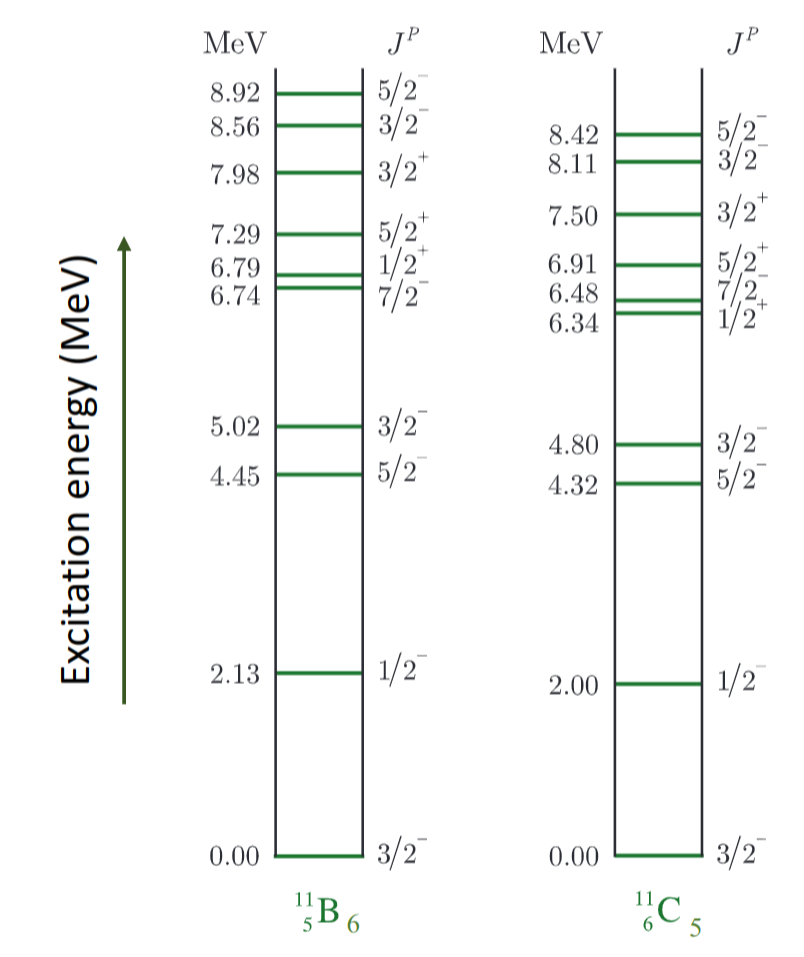
\includegraphics[width = .5\textwidth]{mirror_nuclei_excitation_levels_comparison.png}
    \caption{Comparison of the excitation levels of mirror nuclei. In this case we have $\displaystyle _{5}^{11}\text{B}_{6}$ and $\displaystyle _{6}^{11}\text{C}_{5}$}
    \label{fig: mirror_nuclei_excitation_levels_comparison}
    \end{figure} 
    
\end{itemize}

\subsection{Effects of the Short Range of the Strong Force}
\begin{itemize}
    \item When shooting alpha particles at a nucleus, the alpha particles are repelled by the Coulomb force if they do not have enough energy to get close enough to the nucleus. Then the strong force takes over and the alpha particles are attracted to the nucleus. This is why the Rutherford model does not work at lower energies. 
    \item The linear dependence on the binding energy per nucleon shows that the strong force is short range. If it were long range, each nucleon would attract all the others. Then the term in the binding energy as seen in the first therm of \cref{eq: semi_empirical_mass_formula}, would be quadratic and not linear $(α_vA)$
\end{itemize}

\subsection{Deuteron}
\begin{itemize}
    \item Consist of a proton and a neutron (nucleus of deuterium).
    \item To understand the structure of the atoms we would need to study its excited states. The problem is that deuteron is weakly bound and has no excited states.
\end{itemize}
\subsubsection{Deuteron Binding Energy}
There are multiple ways of calculating the binding energy of the deuteron. 
\begin{enumerate}
    \item \textbf{Mass spectroscopy}: Find the difference in mass between the deuteron and the proton and neutron.
    \begin{equation}
      B = \left( M\left(_{}^{1}\text{H}_{}\right) + m_n - m\left(_{}^{2}\text{H}_{}\right)\right)c^2 = 2.225 \text{ MeV}
    \end{equation} 
    \item \textbf{Nuclear reaction}: The gamma ray emitted when a neutron is captured by a proton is almost the binding energy. It has only energy, but can be converted to mass through $E = mc^2$.
    \begin{align}
    _{}^{1}\text{H}_{}& + n → \ce{_{}^{2}\text{H}_{}} + γ \\ 
    E_{γ} &≈ B = M_{\text{initial}} - M_{\text{final}} \\
    B &= \left( M\left(_{}^{1}\text{H}_{}\right) + m_n - M\left(_{}^{2}\text{H}_{}\right)\right)c^2 = 2.224 \text{ MeV}
    \end{align}
\end{enumerate}

\subsubsection{Nucleon-Nucleon Potential}
\begin{itemize}
    \item We assume that the potential between the nucleons is a finite square well with a potential depth of $-V_0$
    \item Solving for the Schrödinger equation for specific energy values and applying the boundary conditions we get the following results:
    \begin{align}
    &k_1 \cot \left(k_1 \vec{R}\right) = -k_2 \\
    &k_1 = \sqrt{\frac{2mE}{\hbar^2}} \quad k_2 = \sqrt{\frac{2m\left(V_0 + E\right)}{\hbar^2}}
    \end{align}
    \item The radius $R$ is now connected to the energy, and we know from scattering experiments that the radius is around 2.1 fm.
    \item The solution gives a potential of $V_0 = 35$ MeV. 
    \item The binding energy of the deuteron is just below the potential depth as seen in \cref{fig: deuteron_potential}.
    \begin{figure}[h!]
    \centering
    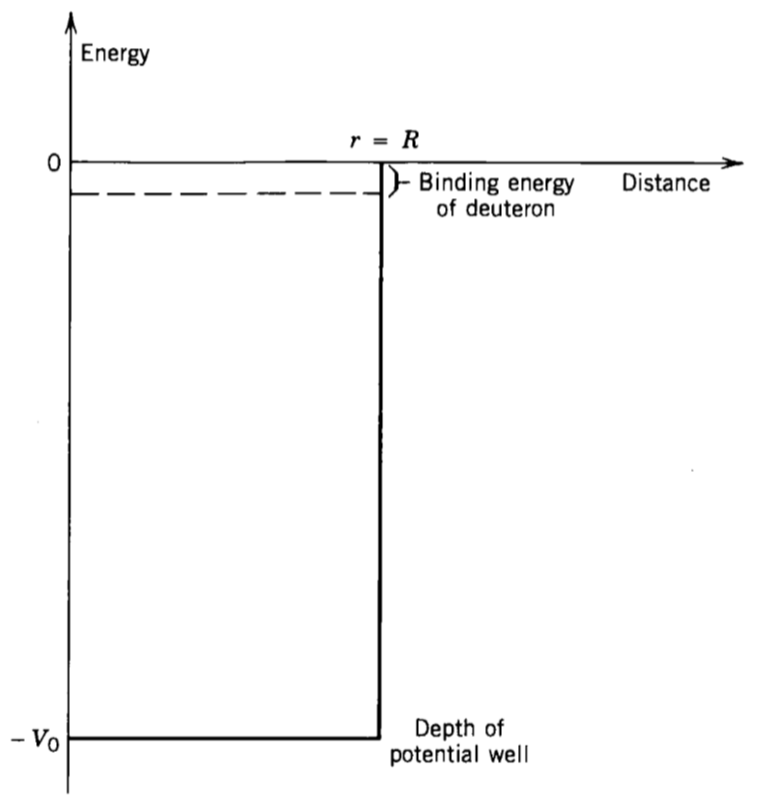
\includegraphics[width = .5\textwidth]{deuteron_potential.png}
    \caption{Square well potential for the deuteron. }
    \label{fig: deuteron_potential}
    \end{figure}
\end{itemize}

\subsubsection{Deuteron Spin and Parity}
\paragraph{Total Spin:}
\begin{equation}
  \vec{I} = \vec{S}_p + \vec{S}_n + \vec{l}
\end{equation}
\paragraph{Spin Configuration with $I = 1$}
\begin{enumerate}
    \item Aligning the spins gives $I = 1$ and $S = 1$ with $l = 0$. This is a positive parity state with $π = (-1)^{l} = 1$. We then get $I^{π}$ 
    \item Aligning the spins with gives $I = 3$
\end{enumerate}

\paragraph{Electric Quadrupole Moment}
The deuteron has a small non-zero electric quadrupole moment. This makes it so about 4\% of the time the deuteron is in an excited state with $l = 2$.  %#  6
\section{The Standard Model}
 %#  7
\subsection{Charges}
\begin{itemize}
    \item The charges are $α_{\text{W}}, α_{\text{W}}, α_{\text{S}}$, for the weak, electromagnetic, and strong force, respectively.
    \item The product of the charges show how likely an interaction is to happen.
\end{itemize}

\subsubsection{Examples}
At the vertices in \cref{eq: charge_1}, we place the charge, $α_{\text{EM}}$, being proportional to the electromagnetic charge squared. 
\begin{equation}\label{eq: charge_1}
e^{-} γ \stackrel{α_{\text{EM}}}{→} e^{-} γ
\end{equation}

We do the same for the strong force in \cref{eq: charge_2}.
\begin{equation}\label{eq: charge_2}
  g \stackrel{α_{\text{S}}}{→} gg
\end{equation}

\subsection{Allowed Vertices (\cref{fig: feynman_diagram_vertices})}
\begin{itemize}
    \item A vertices is where the particle lines meet. 
    \item Processes can in theory be written in reverse. 
    \item Not all vertices are allowed. The $Q$-value must be negative, meaning the process must be energetically allowed.
    \item Quantities like charge, baryon number, lepton number,energy and strangeness must be conserved. 
    \item $e^{+} → e^{+}γ$ would not be allowed as we can pick a frame of reference where the electron is at rest, and the photon would have energy less than or equal to 0.
\end{itemize}

\begin{figure}[h!]
\centering
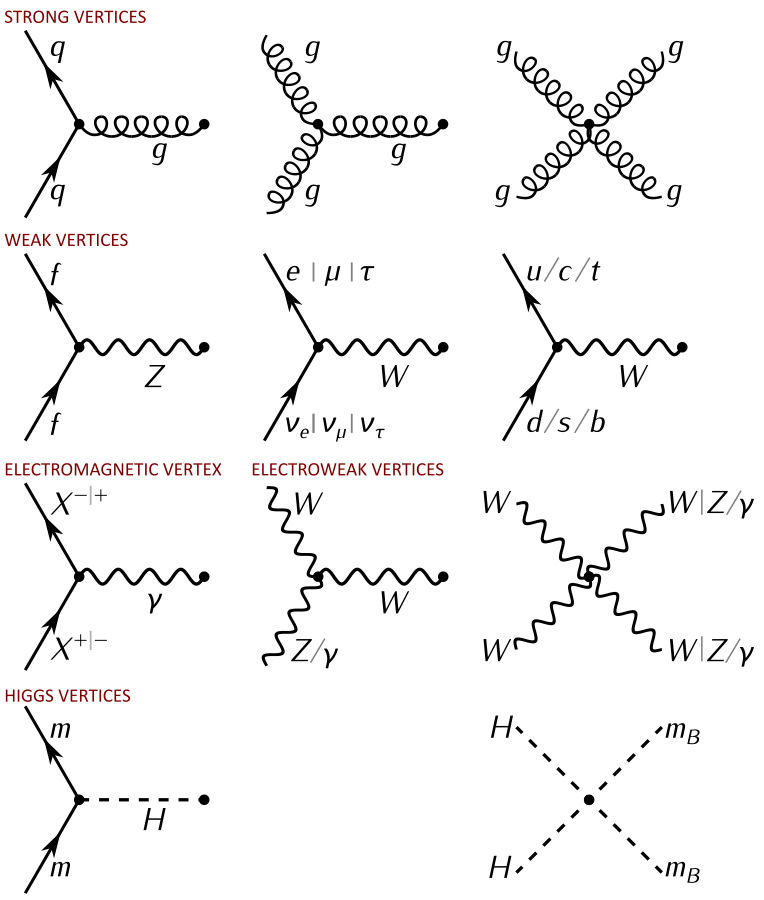
\includegraphics[width = \textwidth]{feynman_diagram_vertices.png}
\caption{Figure of allowed vertices in the Standard Model.}
\label{fig: feynman_diagram_vertices}
\end{figure}


We can change the time ordering in \cref{eq: charge_1}, to the following in \cref{eq: charge_3}. Here the photons comes in and interacts with the electron. This is a non-physical process, as the mass/energy of the system in a rest frame is not conserved. 
\begin{equation}\label{eq: charge_3}
  γ e^{-} \stackrel{α_{\text{EM}}}{→} e^{-} γ
\end{equation}

\subsubsection{Allowed EM Vertices}
\cref{eq: a_EM_v_1} is allowed as a part of a larger process, but not on its own. This is because the mass of the tauon can't increase or decrease, meaning the photon must have a mass (energy) of 0.
\begin{equation}\label{eq: a_EM_v_1}
τ^{+} → τ^{+}γ
\end{equation}

\cref{eq: a_EM_v_2} is allowed as a part of a larger process, but not on its own. Same as \cref{eq: a_EM_v_1}, where the mass of the anti charm quark can't increase or decrease, meaning the photon must have a mass (energy) of 0. 
\begin{equation}\label{eq: a_EM_v_2}
y \bar{c} → \bar{c}
\end{equation}

\cref{eq: a_EM_v_3} is allowed as a part of a larger process, but not on its own. A real photon does not have mass, meaning it cannot create a top quark and an anti-top quark. We could flip one of the vertices to be $γ \bar{t} → \bar{t}$ and we see this to be impossible. 
\begin{equation}\label{eq: a_EM_v_3}
γ → t\bar{t}
\end{equation}

\subsubsection{Allowed Strong Vertices}
\cref{eq: a_strong_v_1} Could be a part of a larger diagram, but can't represent a physical process on its own due to conservation of energy. 
\begin{equation}\label{eq: a_strong_v_1}
  g \bar{c} → \bar{c}
\end{equation}

\cref{eq: a_strong_v_2} This is a possible process, as the gluon can have a high enough mass for this to be possible. 
\begin{equation}\label{eq: a_strong_v_2}
  g → t \bar{t}
\end{equation}

\cref{eq: a_strong_v_3} This is a possible process, as the gluon can interact with it self
\begin{equation}\label{eq: a_strong_v_3}
  g → g g
\end{equation}


\subsubsection{Neutral Weak Vertices}
All vertices with the photon can be interchanged with the $Z^{0}$-boson but NOT the other way around. See \cref{eq: a_weak_v_1} for an example.
\begin{equation}\label{eq: a_weak_v_1}
  γ / Z^{0} → e^{+} e^{-}  
\end{equation}

The neutrino is electrically neutral, and does not interact with the photon, meaning the process in \cref{eq: a_weak_v_2} only works with a $Z^{0}$-boson.
\begin{equation}\label{eq: a_weak_v_2}
  ν_{μ} → ν_{μ}Z^{0}
\end{equation}

As the process is electrically neutral, the $Z^{0}$-boson can be created from the annihilation of a down-type quark and an anti-down-type quark, as seen in \cref{eq: a_weak_v_3}.
\begin{equation}\label{eq: a_weak_v_3}
  d \bar{d} → Z^{+}  
\end{equation}

\subsubsection{Charged Weak Vertices}
The $W^{±}$-boson can interact with all fermions, but as it has a charge, it changes the charge of the particles it interacts with. Net charge must be conserved, meaning the process in \cref{eq: a_weak_v_4} is allowed.
\begin{equation}\label{eq: a_weak_v_4}
  W^{-} → \bar{u} d
\end{equation}

To get zero charge, but keep the number of anti-fermions we can have the process in \cref{eq: a_weak_v_5}.
\begin{equation}\label{eq: a_weak_v_5}
  e^{+}W^{-} → \bar{ν}_{e}
\end{equation}

The electric charge of the $W^{±}$-boson can interact with the photon. This is seen in \cref{eq: a_weak_v_6}.
\begin{equation}\label{eq: a_weak_v_6}
  W^{+} → W^{+}γ
\end{equation}

Net charge is conserved, which allows the process in \cref{eq: a_weak_v_7}.
\begin{equation}\label{eq: a_weak_v_7}
  Z^{0} → W^{+}W^{-}  
\end{equation}

\subsubsection{Higgs Boson Vertices}
The Higgs boson interacts with the mass of fermions, but maybe not the mass of neutrinos. 

\cref{eq: a_higgs_v_1} is a possible process, as the Higgs boson can interact with the mass of the top quark.
\begin{equation}\label{eq: a_higgs_v_1}
  t \bar{t} → H
\end{equation}

\cref{eq: a_higgs_v_2} is a possible process, as the Higgs boson can create the muons, as charge is conserved. 
\begin{equation}\label{eq: a_higgs_v_2}
  H → μ^{+} μ^{-}
\end{equation}

\cref{eq: a_higgs_v_3} is possible, and dependant on the mass of the $Z^{0}$-boson.
\begin{equation}\label{eq: a_higgs_v_3}
Z_0 → Z^{0}H  
\end{equation}

The Higgs boson can interact with itself, as seen in \cref{eq: a_higgs_v_4}.
\begin{equation}\label{eq: a_higgs_v_4}
H → H H
\end{equation} 



 %#  8
\subsubsection{4-Line Vertices}
\begin{itemize}
    \item There is no complete list of all possible 4-line vertices. 
    \item As seen in \cref{fig: feynman_diagram_vertices}, we know that both gluons, Higgs bosons and $W / Z / γ$  bosons can have 4-line vertices. This means two particles can scatter, creating two new particles, without an intermediate particle.
    \item This is caused by particles being able to interact with themselves. 
    \item These are rarely used
\end{itemize}

\subsection{Creating Feynman Diagrams}
Often there are multiple ways to describe the same process. There can be multiple different time orders. Example can be seen in \cref{eq: moeller_scattering}, visualized in two different ways in \cref{fig: moeller_scattering}. This is not always done as it is implied that both are possible, and you need to calculate both. A time independent version can be seen in \cref{fig: moeller_scattering_time_independat}.

\begin{equation}\label{eq: moeller_scattering}
    e^{-} e^{-} → e^{-} e^{-}
\end{equation}

\begin{figure}[ht!]
\centering
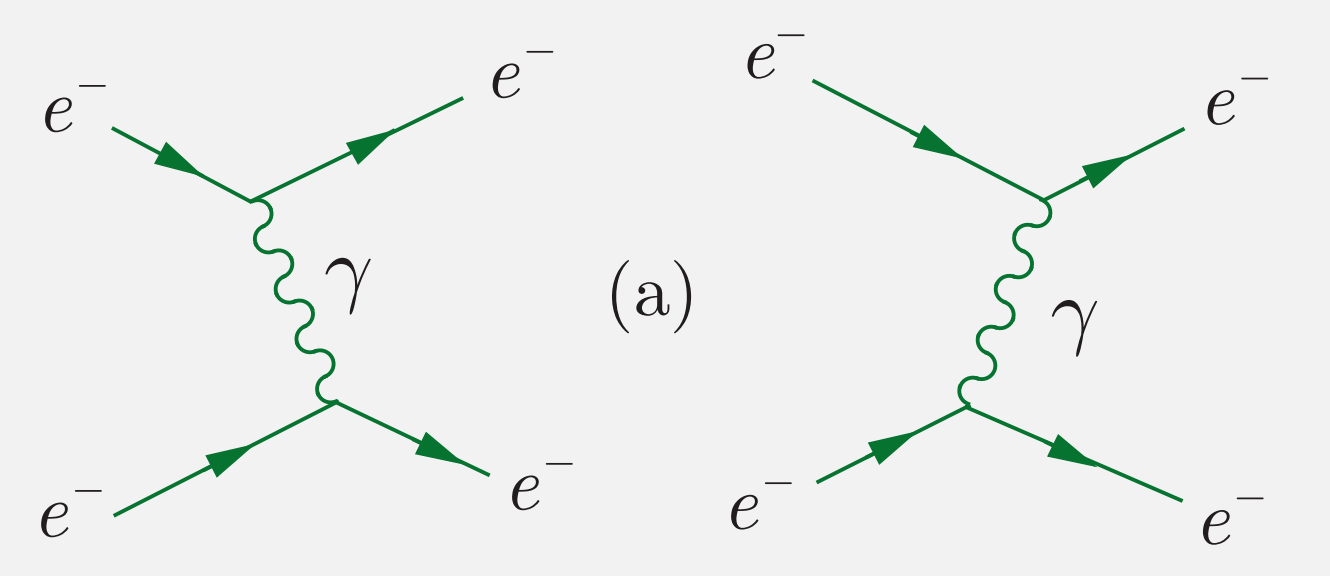
\includegraphics[width = .75\textwidth]{moeller_scattering.png}
\caption{Two different ways to visualize Møller scattering as seen in \cref{eq: moeller_scattering}.}
\label{fig: moeller_scattering}
\end{figure}

\begin{figure}[h!]
\centering
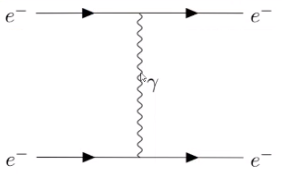
\includegraphics[width = .6\textwidth]{moeller_scattering_time_independat.png}
\caption{A time independent version of Møller scattering as seen in \cref{eq: moeller_scattering}.}
\label{fig: moeller_scattering_time_independat}
\end{figure}


\subsubsection{Tip for Choosing Time-Ordering}
Just pick one and see if the charge and all other properties are conserved. As seen in \cref{fig: time_ordering_example}, we can choose the time ordering based on the charge conservation. Only the electron can emit the negatively charged $W^{-}$-boson. Therefore, the emission on the bottom happens before absorption on the top. The unambiguous time ordering can be seen in \cref{fig: time_ordering_example_solved}. We could of course have flipped the figure horizontally. 

\begin{figure}[h!]
\centering
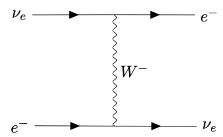
\includegraphics[width = .6\textwidth]{time_ordering_example.png}
\caption{Example showing a case were logic is used to choose the time ordering.}
\label{fig: time_ordering_example}
\end{figure}

\begin{figure}[h!]
\centering
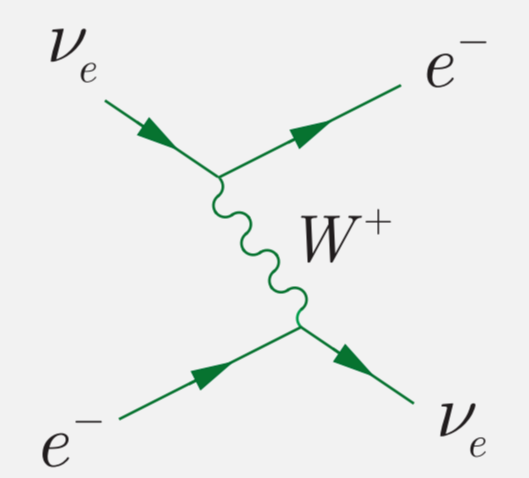
\includegraphics[width = .6\textwidth]{time_ordering_example_solved.png}
\caption{Solved case of ambiguity in time ordering from \cref{fig: time_ordering_example}.}
\label{fig: time_ordering_example_solved}
\end{figure}

\subsubsection{Current interactions}
\begin{itemize}
    \item Fermion lines must be continuous. 
    \item Anti-fermion lines must be continuous.
\end{itemize}

\section{Relativity and Anti-Particles}
\subsection{Dirac Equation}
\begin{itemize}
    \item A relativistic equation for the electron.
    \item Makes a prediction of the positron (anti-electron). 
    \item All charged particles have an anti-particle $(p, \bar{p})$, $(μ^{-}, μ^{+})$
    \item For neutral particles, their respective anti-particles have the same charge, but their quarks are opposites (neutrons), or they are their own anti-particle (photons).
    \item Predicts a relation between spin $\vec{S}$ and magnet moment $\vec{μ} = \vec{qS} / m$. This has been confirmed for the electron and muon, but not for protons and neutrons. This hints at the existence of substructure in protons and neutrons.
\end{itemize}

\subsection{Symmetries and Conservation Laws}
\subsubsection{Symmetries and Conserved Quantities}
Noethers theorem states that for every continuous symmetry, there is a conserved quantity. A list of symmetries and their conserved quantities can be seen in \cref{tab: symmetries_table}. They all have their quantum operators. If the physics remains unchanged under a transformation, the system is said to be symmetric under that transformation.

\begin{table}[h!]
\centering
\begin{tabular}{ |c|c|c| }
    \hline
    \textbf{Symmetry} &\textbf{Conserved Quantity} &\textbf{Interactions} \\ 
    \hline
    Space translation &Linear momentum &All \\ 
    Space rotation &Angular momentum &All \\ 
    Time displacement &Energy &all \\ 
    Space inversion &Parity &Not weak \\ 
    Charge inversion &C-parity &Not weak \\ 
    u <-> d &Isospin &String \\ 
    \hline
    \end{tabular}\label{tab: symmetries_table}
\end{table}

\subsubsection{Intrinsic Parity}
\begin{itemize}
    \item All particles at rest have intrinsic parity. This comes from a the only eigenvalue of the parity operator $\hat{P}$ acting on a plane wave function $Ψ(\vec{r},t) = \exp \left(i(\vec{r} ⋅ \vec{p} - Et) / h\right)$, can only return the same wavefunction if $\vec{p} = 0$. 
    \item By convention, we say fundamental fermions have $P = +1$, and their antiparticles have $P = -1$. This is arbitrary. 
\end{itemize}

\subsubsection{Parity of Bound States}
In quantum mechanics we can split the spatial part of the wave function into a radial part $R(r)$ and a spherical harmonic $Y_{l}^{m}(\theta, \phi)$. 
\begin{equation}
Ψ = R_{nl}(r) Y_{l}^{m}(\theta, \phi)
\end{equation}
\begin{equation}
\vec{r} → - \vec{r} \quad ⇒ \quad  r → r, θ → π - θ, ϕ → ϕ + π
\end{equation}
The parity of the spherical harmonic is $(-1)^{l}$. 

\subsubsection{Charge Conjugation}
\begin{itemize}
    \item The charge conjugation operator $\hat{C}$ changes all particles to their antiparticles.
    \item Eigenstates of $\hat{C}$ are particles that are their own antiparticles, like photons. 
    \item Eigenvalues are $\pm 1$. 
\end{itemize}

\subsubsection{Natural Units}
\begin{itemize}
    \item To make life simple we let $ℏ = c = 1$, and only add them back at the end when knowing the units. 
    \item All quantities are measured in energy $\left(eV\right)^{n}$. 
    \item Energy: $eV$
    \item Momentum: $eV / c$
    \item Mass: $eV / c^2$
    \item Time and length: $1 / eV$
    \item It is useful to memorize $ℏc ≈ 197 MeVF$
\end{itemize}

\subsection{Scattering}
\begin{itemize}
    \item Scattering experiments is the core of nuclear and particle physics. 
    \item Elastic Scattering: Same particles in the initial and final state. An example can be seen in \cref{eq: elastic_scattering_example}, where a proton and electron collide. The electron might lose some energy in the form of momentum to the proton, but the particles are the same and their center of mass is unchanged. 
    \begin{equation}\label{eq: elastic_scattering_example}
        e^{-} p → e^{-} p
    \end{equation}
    \item Inelastic Scattering: Different particles in the initial and final state. An example can be seen in \cref{eq: inelastic_scattering_example}, where a particle can collide with an atom and excite it to a higher energy state.
    \begin{equation}\label{eq: inelastic_scattering_example}
        a A → a + A^{*}
    \end{equation}
\end{itemize}

\subsubsection{Decay}
\begin{itemize}
    \item Unstable parent particles decay into stable and lighter daughter particles. 
    \item Atom decay: $A^{*} → A + γ$
    \item Neutron decay: $n → p + e^{-} + \bar{ν}_{e}$
    \item $Z^{0}$ boson decay: $Z^{0} → e^{+} + e^{-}$. 
    \item For free particles, we must have a positive Q-value defined in \cref{eq: Q_value}.
    \begin{equation}\label{eq: Q_value}
        Q = \left(M_{\text{P}} - ∑_{i}^{} M_{\text{D}_i}\right)c^2
    \end{equation} 
    \item For unstable nuclei and particles we have a decay rate as seen in \cref{eq: decay_rate}.
    \begin{equation}\label{eq: decay_rate}
        \frac{dN(t)}{dt} = -λN(t)
    \end{equation}
    The decay constant $λ$ is related to the half-life $T_{1/2}$ by $λ = \ln(2) / T_{1/2}$, with units of $s^{-1}$. 
    \item The mean lifetime is given by $τ = 1 / λ$. This represent the average time a particle will live before decaying. The mean lifetime refer to the rest frame of the particle. 
    \item Decay Width $Γ$: The decay rate in natural units. It is related to the decay constant by $Γ = ℏλ$.
    \item Decay Channels: The different particles a particle can decay into. Each has its own decay width, where the total decay width is the sum of all the decay widths $Γ = ∑_{i}^{} Γ_i$. Each channel has the same mean lifetime. They live for the same amount of time, but the probability of decaying into a specific channel is different. 
    \item Branching Fraction: The probability of a particle decaying into a specific channel, given by $B = Γ_{i} / Γ_{\text{tot}}$.
\end{itemize}




 %#  9
\subsection{Cross-Section}
\begin{itemize}
    \item We measure the rate $W$ of a process happening. 
    \item The number of particles hitting a target per unit area is called flux $J = n_{b} v_i$, where $n_{b}$ is the number of particles per unit volume and $v_i$ is the velocity of the beam. 
    \item The area per target particle is called the cross section $σ$. This represents the area in which the particles interact in the relevant process.
    \item The rate of particles hitting the target is $W = JNσ$. where $N$ is the number of particles. 
    \item The rate $W$ is proportional to the luminosity $L$ by $W = L(t)σ$. 
    \item The cross section $σ$ is invariant under Lorentz transformations in the direction of the beam, meaning it is independent of the reference frame. 
    \item Colliding two beams beams of $N_1$ number of particles and $N_2$ number of particles, we get a luminosity $L(t) = f N_1 N_2 / A$, where $f$ is the frequency of the beam (how often they collide) and $A$ is the area of the beam.
\end{itemize}

\subsubsection{Differential Cross-Section}
Measured time-integrated rate as a function of some observable. This could be momentum: 
\begin{equation}
    σ = ∫_{p_{\text{min}}}^{p_{\text{max}}} \frac{\mathrm{d}σ(p)}{\mathrm{d}p} \ \mathrm{d}p
\end{equation}

\subsubsection{Measured Cross-Section}
\begin{enumerate}
    \item Define the process of interest. 
    \item Count the number of times the process happens.
    \item Remove the background noise as measurement is imperfect. 
    \item Find the time-integrated luminosity $\mathcal{L} ≡ ∫  L(t) \mathrm{d}t$. 
    \item For the total cross-section, we have $N = σ \mathcal{L}ϵ + b$ or $\displaystyle σ = \frac{N - b}{\mathcal{L}ϵ}$, where $ϵ$ is the efficiency of the detector and $b$ is the background noise.
\end{enumerate}

\subsubsection{Integrated Luminosity}
\begin{itemize}
    \item One can either precisely control the details of the beam and target to determine $\mathcal{L}$.
    \item One can also used well-known processes to determine $\mathcal{L} = N_1 / σ_1$, if this event has a known cross-section. After that, one can correct for noise and efficiency, to then find the cross-section of the process of interest by $σ_2 = \frac{N_2}{\mathcal{L}} = \frac{N_2}{N_1} σ_1$
    \item Barn: Unit of cross-section, $1 \text{b} = 10^{-24} \text{cm}^2$ or $1 \text{b} = 10^{-28} \text{m}^2$. Integrated luminosity is often given in $\text{fb}^{-1}$ or $\text{pb}^{-1}$, where f $(10^{-15})$ and p $(10^{-12})$ stands for femto and pico, respectively. $1\text{pb} ≈ 10^{-40}\text{m}^2 = (10^{-5}\text{fm})^2$. In comparison the proton has a radius of about $0.84\text{fm}$.
\end{itemize}


\subsubsection{Single Beam Particle and Target}
\begin{itemize}
    \item Again we use that the rate of observing some scattering process $r$ is $W_r = JNσr$. 
    \item In the case of a single target particle we have $N = 1$. 
    \item The flux $J = n_{b} v_i$ where $n_{b}$ is the number of beam particles per unit volume $V$ and $v_i$ is the velocity of the beam. 
    \item The differential rate of observing the process $r$ in a solid angle at direction $(θ,ϕ)$, is therefore $ \displaystyle \mathrm{d}W_r = v_\frac{i}{V} \frac{\mathrm{d}σ_r(θ,ϕ)}{\mathrm{d}Ω}dΩ$
\end{itemize}

\subsubsection{Born Approximation}
\begin{itemize}
    \item Assuming the particle has a wavefunction traveling a large distance around the accelerator, we can describe it as a plane wave $ψ_i$. 
    \item When disturbed by a potential $V(r)$, we can calculate the rate of scattering by the Born approximation. This is also known as "Fermi's Golden Rule". If we define the probability amplitude $\mathcal{M}(\vec{q})$, we get from \cref{eq: fermis_golden_rule} that the rate of scattering is given by \cref{eq: fermis_golden_rule_2}. Here $\vec{q}$ is the momentum transferred. 
    \begin{equation}\label{eq: fermis_golden_rule}
      \mathrm{d}W_r = \frac{2π}{ℏ} \left|∫ ψ_f^{*}V(\vec{r})ψ_i \mathrm{d}^3 \vec{r}\right| ρ(E_f) 
    \end{equation}
    \begin{equation}\label{eq: fermis_golden_rule_2}
      \mathrm{d}W_r = \frac{2π}{ℏ} \left|M(\vec{q})\right|^2 ρ(E_f), \quad M ≡ ∫ V(\vec{r})\exp \left(i \vec{q} ⋅ \vec{r} / ℏ\right)d^3 \vec{r}
    \end{equation}
    \item Multiplying by $ℏ^2c^2$ which we know to be about $(197 \text{ MeV F})^2$ we cancel out the energy and get $σ$ in units of $\text{F}^2$ aka barn. 
\end{itemize}

\subsubsection{Natural Units and Cross Section}
\begin{itemize}
    \item Cross-sections $σ$ has unit of area, barn (b) of $10^{-28}$ m$^2$. 
    \item In natural units this is proportional to $1 / E^2$ with units $1 / $MeV$^2$
\end{itemize}

\subsection{Density of States (Energy States)}
The number of states in a range of momenta $d^3 \vec{p}$. This is derived from a wavefunction in a box of volume $V = L^3$ with walls of infinite potential. The coordinate system is places in one of the corners such that the walls are at $x = L$, $y = L$ and $z = L$. From this we get the density of states in momentum space $d^3 \vec{p}$ as seen in \cref{eq: density_of_states}.
\begin{equation}\label{eq: density_of_states}
 ρ(E) \mathrm{d}q = \frac{L^3}{(2πℏ)^3} d^3 \vec{p} \quad , \quad  → \mathrm{d}^3 \vec{p} = q^2 \ \mathrm{d}q \ \mathrm{d}ϕ \ \mathrm{d}(\cos ϕ) ≡ q^2 \mathrm{d}q \mathrm{d}Ω
\end{equation}
\cref{eq: density_of_states} can be used further where \cref{eq: density_of_states_2} is defined. Now we need to find $\frac{\mathrm{d}q}{\mathrm{d}E}$
\begin{equation}\label{eq: density_of_states_2}
    ρ(q)\mathrm{d}q ≡ ρ(E)\mathrm{d}E → ρ(E) = ρ(q) \frac{\mathrm{d}q}{\mathrm{d}E} = \frac{L^3}{(2πℏ)^3} q^2 \frac{\mathrm{d}q}{\mathrm{d}E} \mathrm{d}Ω
\end{equation}
\paragraph{Non-Relativistic Case:}
\begin{itemize}
    \item $E = q^2 / 2m$
    \item $\mathrm{d}E = 2q \mathrm{d}q / 2m = q \mathrm{d}q /m$
    \item \textbf{Conclusions:} $\frac{\mathrm{d}q}{\mathrm{d}E} = m / q = 1 / v$
\end{itemize}

\paragraph{Relativistic Case:}
\begin{itemize}
    \item $E^2 = m^2c^{4} + q^2 c^2$
    \item $2E \mathrm{d}E = 2c^2 q \mathrm{d}q$
    \item \textbf{Conclusions:} $\frac{\mathrm{d}q}{\mathrm{d}E} = E / qc^2 = mγc^2 / mγβc^3 =  \frac{1}{ βc} = 1 / v$
    The result is the same!
\end{itemize}

\subsubsection{Conclusion}
\begin{equation}
\frac{\mathrm{d}σ_r(θ,ϕ)}{\mathrm{d}Ω} = \frac{1}{(2π^2)} \frac{1}{ℏ^{4}} \frac{q_f^2}{v_f v_i} \left|M(\vec{q})\right|^2
\end{equation}

\subsection{Theoretical Cross-Section for $ab → cd$}
\begin{itemize}
    \item The differential cross-section for a process $ab → cd$ is given by \cref{eq: differential_cross_section}, where $g_i$ and $g_f$ are number of spin-states for the initial and final states particles, respectively. $g_f = (2S_{c} + 1)(2S_{d} + 1)$ and $g_i = (2S_{a} + 1)(2S_{b} + 1)$. $k$ represent all possible spin states. 
    \begin{equation}\label{eq: differential_cross_section}
    \frac{\mathrm{d}σ}{\mathrm{d}Ω} = \frac{g_f}{4π^2ℏ^{4}} \frac{q_f^2}{v_i v_f} \overline{|M(\vec{q})|^2} \quad , \quad  \overline{|M(\vec{q})|^2} = \frac{1}{g_i g_f} ∑_{k}^{} \left|M_k\right|^2
    \end{equation}
    \item In general, the particle beams are unpolarized and we therefore do not measure the spin of the final state particles. 
    \item We average over the initial spin states, and sum over the final ones. 
\end{itemize}

\section{Particle Phenomenology}
\subsection{Leptons}
\begin{itemize}
    \item 3 generations increasing in mass. 
    \item Neutrinos has only weak interactions due to lack of charge. This makes it has to detect and is a hint of a weak interaction. 
    \item Except a few cases, the generations of leptons are conserved in interactions.
    \item The weakness of the weak force comes from the massive mediating particles $W^{\pm}$ and $Z^{0}$. 
    \item The flavour of the lepton does not affect the strength of the interaction. 
\end{itemize} %# 10
\section{Range of Forces and Amplitudes}
\subsection{Yukawa Potential}
Looking at the Schrödinger equation:
\begin{equation}
  H Ψ = E Ψ
\end{equation}
where the energy solution must satisfy $E^2 = m^2c^{4} + p^2c^2$.  The energy and momentum operators are given by:
\begin{equation}
    E = iℏ \frac{∂}{∂t} \quad , \quad \vec{p} = -iℏ \vec{∇}
\end{equation}
The solution should $ϕ$ be a static one, representing a radial potential:
\begin{equation}
  ∇^2ϕ(r) = \frac{m^2c^2}{ℏ^2} ϕ(r)
\end{equation}
As the factors have units of length squared, we can create a new variable $R = ℏ^2 / m^2c^2$. Guessing a solution on the form $ϕ(r) = u(r) / r$, we get the following solution not diverging for large $r$:
\begin{equation}
  \frac{∂^2 u(r)}{∂ r^2} = \frac{u(r)}{R^2} →  u(r) = ae^{-r / R} →  ϕ(r) = a \frac{e^{-r / R}}{r}
\end{equation}
This gives a potential $V$ as seen in \cref{eq: yukawa_potential}, with a potential vanishing for large distances. For complex structures we need to take into the internal structure as well. This assumes an interaction between a particle with charge $-g$, and another much heavier particle with charge $+g$.
\begin{equation}\label{eq: yukawa_potential}
  V(r) = -\frac{g^2}{4π} \frac{e^{-r / R}}{r}
\end{equation}

\subsection{Yukawa Amplitude}
Amplitude from the Bourne approximation:
\begin{equation}
  \mathcal{M} = ∫ V(\vec{r}) e^{i \vec{q} ⋅ \vec{r} / ℏ} d^3r  \quad , \quad  \vec{q} = \vec{p}_f - \vec{p}_i
\end{equation}
Solving this with the Yukawa potential, we get the following result:
\begin{equation}
  \vec{q} ⋅ \vec{r} = qr \cos θ \quad , \quad  \mathrm{d}^3r = r^2 \mathrm{d}r = \sin \mathrm{d}θ \mathrm{d}r \mathrm{d}ϕ
\end{equation}
This gives the following result in \cref{eq: yukawa_amplitude}, only valid when $\left|\vec{q}_i\right| = \left|\vec{q}_f\right|$ and energy is constant (elastic scattering):
\begin{equation}\label{eq: yukawa_amplitude}
  \mathcal{M}(q^2) = - \frac{g^2 ℏ^2}{q^2 + m^2c^2}
\end{equation}

To make this Lorentz invariant (as momentum is dependant on the frame of reference), we get the following result in \cref{eq: yukawa_amplitude_lorentz}, when $Q^2 ≪ m^2$
\begin{equation}
  Q^2 (\vec{q}_i - \vec{q}_f)^ - (E_f - E_i)^2 / c^2
\end{equation}
\begin{equation}\label{eq: yukawa_amplitude_lorentz}
  \mathcal{M}(Q^2) = - \frac{g^2 ℏ^2}{Q^2 + m^2c^2}
\end{equation}
If the range of the exchange is very small, then $Q^2$ is also very small, giving us the following approximation:
\begin{equation}
  \mathcal{M}(Q^2) = - \frac{g^2 ℏ^2}{m^2c^2} ≡ -G
\end{equation}
We often visualize this in Feynman diagrams as shown in \cref{fig: non_approx_exhange,fig: approx_exchange} . Both $Q^2$ and $G$ are Lorentz invariant. 
\begin{figure}[h!]
\centering
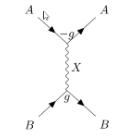
\includegraphics[width = .35\textwidth]{non_approx_exhange.png}
\caption{Feynman diagram of a non-approximated exchange of particle $X$}
\label{fig: non_approx_exhange}
\end{figure}

\begin{figure}[h!]
\centering
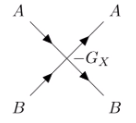
\includegraphics[width = .35\textwidth]{approx_exchange.png}
\caption{Feynman diagram of an short-range approximated exchange of particle $X$}
\label{fig: approx_exchange}
\end{figure}

\subsection{Amplitude of $W$-boson Exchange}
As the result of the short-range approximation shows in \cref{eq: yukawa_amplitude_lorentz}, we see it is dependant on mass, an therefore we can use this to calculate the mass of the $W$-boson. The amplitude of the $W$-boson exchange is given by:
\begin{equation}
  α_{W} ≡ \frac{g^2_{W}}{4πℏc}  \quad , \quad  α_{EM} = \frac{e^2}{4πϵ_0ℏc}
\end{equation}
Taking into account the spins of the particles gives a factor of $\sqrt{2}$. 
\begin{equation}
  G_{F} ? \frac{g^2_{W}ℏ^2}{m^2_{W}c^2}\sqrt{2} → \frac{G_{F}}{(ℏc)^3} = \frac{4πα_{W}}{(m_{Wc^2})^2} \sqrt{2}
\end{equation}
By measurement of $G_{F} / (ℏc)^3 = 1.166 ⋅  10^{-5}$ GeV$^{-2}$, we can calculate the mass of the $W$-boson to be $m_{W} ≈ 105$ GeV/c$^2$, which is close to the actual value of $m_{W} = 80.4$ GeV/c$^2$. This assumes $α_{W} ≈ α_{EM}$. 

\subsection{Amplitude of Other exchanges}
Each vertex has a factor charge and a cross section decay rate which is proportional to $\left|\mathcal{M}\right|^2$. We can count the number of exchanges of particle $X$ as orders of $α_{X}$ ($\sqrt{α_{X}}$, per vertex before squaring). This typically represent small corrections as $α_{X} ≪ 1$. 

\subsection{Muon vs Tau Decays}
\begin{equation}
  μ^- → e^- + \bar{ν}_e + ν_μ
\end{equation}
\begin{equation}
  τ^- → e^- + \bar{ν}_e + ν_τ
\end{equation}
The width of the decay rate is proportional to the matrix elements square: $Γ \propto \left|\mathcal{M}\right|^2$ and $\mathcal{M} \propto G_{F}, G_{f} = 1.166 ⋅  10^{-5} (ℏc)^3 /$GeV$^2$. To get units of energy we must have 
\begin{equation}
  Γ = K G^2_{F}(m_lc^2)^{5} / (ℏc)^{6}
\end{equation}
where $m_l$ is the mass of the initial lepton. We do not need to know $K$ as we only want to compare the two processes. In natural units we get:
\begin{equation}
  KG^2_{F} m_l^{5}
\end{equation}
The ratio then becomes as shown in \cref{eq: muon_tau_ratio}. As the muon only have one decay channel, it is easy to find the decay width. This does not hold for the tau, as it only becomes an electron about 18\% of the time.
\begin{equation}\label{eq: muon_tau_ratio}
  \frac{Γ(τ^{-} → e^{-} \bar{ν}_e ν_{τ})}{Γ(μ^{-} → e^{-} \bar{ν}_e ν_{μ})} ≈ \left(\frac{m_τ}{m_μ}\right)^{5} ≈ 1.354 ⋅  10^{6}
\end{equation}
We must correct for the fact that the tau decays into a muon about 17.8\% of the time, by using their respective lifetime $τ ≡ \frac{1}{Γ}$. Fort he muon we have $\frac{1}{τ_{μ}} = 1 / 2.2 μ$ seconds, and fore the tau we have $\frac{1}{τ_{τ}} = 1 / 0.29 p$ seconds. Using experiment telling us the branching fraction of the tau, we find we a good estimate of the ratio in \cref{eq: muon_tau_ratio}.
\begin{equation}
  \frac{Γ(τ^{-} → e^{-} \bar{ν}_e ν_{τ})}{Γ(μ^{-} → e^{-} \bar{ν}_e ν_{μ})} = \frac{τ_{μ}}{τ_{τ}} \underbrace{B(τ^{-} → e^{-} \bar{ν}_e ν_{τ})}_{17.8 \%} = 1.35 ⋅  10^{6} 
\end{equation}
which is very good estimate within $2\%$ of the predicted value. 


\section{Resonance Formation and Decay}
\begin{itemize}
  \item Cross-section is proportional to the following:
  \begin{equation}
    σ \propto χ^{*}(E) χ(E) \quad , \quad  χ(E) ∫_{0}^{∞} Ψ(t)e^{iωt} \ \mathrm{d}t  ω = E / ℏ
  \end{equation}
  \item The center of mass of the particle has 0 momentum. This gives:
  \begin{equation}
    Ψ(t) = Ψ(0) e^{-iω_{R}t} e^{- Γt / 2} \quad , \quad  ω_{R} = E_{r} / ℏ = m_{R}c^2 / ℏ
  \end{equation}
  \item The result is 
  \begin{equation}
    χ^{*}(E) χ(E) ∝ \frac{1}{(E - m_{R}c^2)^2 + ℏ^2 Γ^2 / 4}
  \end{equation}
  \item Visualized it looks like a Gaussian curve, but with a much higher peak. This is called a Breit-Wigner formula as shown in \cref{fig: breit-wigner_formula}. It tells us the width of the decay rate $Γ$ in energy units, and lets us look at decay rates of particles with very short lifetimes.
  \begin{figure}[h!]
  \centering
  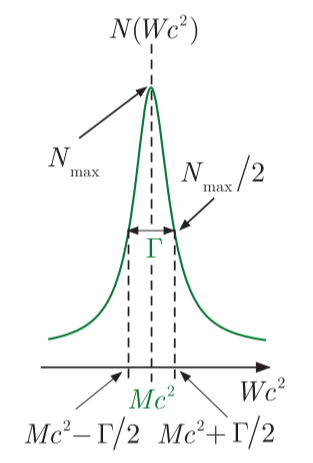
\includegraphics[width = .35\textwidth]{breit-wigner_formula.png}
  \caption{The Breit-Wigner formula for resonance formation and decay}
  \label{fig: breit-wigner_formula}
  \end{figure}
\end{itemize}
\subsubsection{Width and Lifetime}
\begin{itemize}
  \item In practical units: $λ ≡ Γ = 1 / τ$. 
  \item In natural units (energy in this case) : $Γ = ℏ / τ = ℏc / τc$
  \item The wider the width, the shorter the lifetime. 
\end{itemize}

\section{Neutrino Mixing and Oscillations}
\begin{itemize}
  \item Slowly, the neutrinos changes into each other. 
  \item The flavour eigenstates are not the same as their mass eigenstates. 
  \item The neutrinos propagate as mass eigenstates, but are produced and detected as flavour eigenstates of the weak interaction. 
\end{itemize}

\subsection{Neutrino Mixing}
\begin{itemize}
  \item This has an extremely low probability of happening, and has not been observed in the lab.
\end{itemize}
\subsubsection{3-generation mixing}
\begin{itemize}
  \item Easier to understand with 2 generations.
  \item If we produce a beam of $ν_e$ with momentum $p$, we can observe it later at some distance $x$. 
  \item As the neutrinos are produced as a mix of mass eigenstates, they will propagate slightly differently because of their mass difference. Some will turn into $ν_μ$, written as: $ν_e →  ⊗  → ν_{μ}$
\end{itemize}

\subsection{Probability of Mixing}
Starting with a beam of only $ν_e$ at $t = 0$. We can calculate the time dependent state. 
\begin{equation}
  \begin{pmatrix*}[r]
   \ket{ν_e} \\
   \ket{ν_{μ}} \\
  \end{pmatrix*} = 
  \begin{pmatrix*}[r]
   \cos θ & \sin θ \\
   -\sin θ & \cos θ \\
  \end{pmatrix*}
  \begin{pmatrix*}[r]
   \ket{ν_1} \\
   \ket{ν_{2}} \\
  \end{pmatrix*} \quad \text{and} \quad  
  \begin{pmatrix*}[r]
    \ket{ν_e} \\
    \ket{ν_{μ}} \\
   \end{pmatrix*} = 
   \begin{pmatrix*}[r]
    \cos θ & -\sin θ \\
    \sin θ & \cos θ \\
   \end{pmatrix*}
   \begin{pmatrix*}[r]
    \ket{ν_1} \\
    \ket{ν_{2}} \\
   \end{pmatrix*}
\end{equation}
\begin{equation}
  \ket{ν(t)} = a(t) \cos θ \ket{ν_1} + b(t) \sin θ \ket{ν_2} \quad , \quad  a(t) = \exp \left(-i E_1 t\right) \ , \ b(t) = \exp \left(-i E_2 t\right)
\end{equation}
As we can both detect $ν_e$ and $ν_{μ}$, we can calculate each probability, with a superposition of their wavefunctions instead of $ν_1$ and $ν_2$. 
\begin{equation}
  \ket{ν(t)} = a(t) \cos θ \left(\cos θ \ket{ν_e} - \sin θ \ket{ν_{μ}}\right) + b(t) \sin θ \left(\sin θ \ket{ν_e} + \cos θ \ket{ν_{μ}}\right)
\end{equation} 
\begin{equation}
  \ket{ν(t)} = \Big(a(t) \cos ^2 θ + b(t)\sin ^2 θ\Big)\ket{ν_e} + \Big(b(t) \sin θ \cos θ - a(t) \sin θ \cos θ\Big) \ket{ν_{μ}}
\end{equation}
Only if $a = b$ for all $t$, there will be no mixing. The normalization is defined as:
\begin{equation}
  \left|\bra{ν_e}\ket{ν_e}\right|^2 ≡ \left|\bra{ν_{μ}}\ket{ν_{μ}}\right|^2 ≡ 1
\end{equation}

The probability of finding the muon neutrino is given by:
\begin{equation}
  P(ν_{μ}) = \left|\bra{ν_{μ}}\ket{ν(t)}\right|^2 = \left|\frac{b(t) - a(t)}{2}\right|^2 \sin ^2 2θ \quad , \quad  \text{using } \sin 2θ = 2 \sin θ \cos θ
\end{equation}
\begin{equation}
  \left|b(t) - a(t)\right|^2 = b^{*}b + a^{*}a - (a^{*}b + b^{*}a) = 2 - \exp \left(i(E_2 - E_1)t\right) - \exp \left(-i(E_2 - E_1)t\right)
\end{equation}
Using the fact that $\exp ix + \exp -ix = 2 \cos x$ and $\sin ^2 x / 2 = (1 - \cos x) / 2$ we get:
\begin{equation}
  2 - 2 \cos \left(E_2 - E_1\right)t = 4 \sin ^2 \left(\frac{E_2 - E_1}{2}t\right)
\end{equation}
We finally get the probability:
\begin{equation}
\underline{\underline{ P(ν_{μ}) = \left|\bra{ν_{μ}}\ket{ν(t)}\right|^2 = \sin^2θ\sin^2 \left(\frac{(E_2 - E_1)t}{2}\right)}}
\end{equation}
As long as $θ$ is nonzero, or the energies are equal, we get a probability oscillating between 0 and 1.

\subsubsection{Conclusion}
\begin{itemize}
  \item As the masses of the neutrinos are very small in comparison to their momentum, we say the energy is the momentum. This gives a new difference in energy:
  \begin{equation}
    E_2 - E_1 = \frac{m_2^2 - m_1^2}{2E}
  \end{equation} 
  \item for small masses, $v ≈ c$, so the position $L(t) \approx ct$. 
  \item We define a new constant in natural units $L_0 ≡ 4E / (m_2^2 - m_1^2)$
  \item We have a final result of the probability of oscillation as:
  \begin{equation}
    P(ν_{μ}) = \sin^2 2θ \sin^2 \left(\frac{L}{L_0}\right)
  \end{equation}
  \item The scale of these oscillations are very large, and therefore very hard to detect. 
\end{itemize} %# 11
\section{Nuclear Models}
\begin{itemize}
    \item Two main categories, single particle, and collective. 
    \item Collective models looks at the nucleas as a whole. Single particle models looks at the nucleas as a collection of individual particles.
\end{itemize}

\subsection{Liquid-Drop Model}
\begin{itemize} 
    \item A collective model. 
    \item Assumes the nucleus behaves like molecules in an oscillating drop of liquid.
    \item All molecules attract eachother and are held together by surface tension. 
    \item The droplet is charged which destabilizes the oscillations. 
    \item Heavy droplets are shaped like dumbbells, as they are almost split in two. 
    \item The models explains the binding energy and mass of the nuclei. It also explains the fission of heavy nuclei.
    \item The model does not explain the shell structure or magic numbers  
\end{itemize}

\subsection{Fermi-Gas model \cref{fig: Fermi-Gas_model}}
\begin{itemize}    
    \item A single particle model.
    \item Consider a system of completely non-interacting nucleons in a three dimensional box potential. 
    \item The potential is a well-potential, which treats protons and neutrons differently. The protons has a lower potential than the neutrons. 
    \item The nucleons are arranged in pairs because of the Pauli exclusion principle. 
    \item The Fermi energy $E_{F}$ is the energy of the highest occupied state.
    \item The Fermi momentum $p_{F}$ is the momentum of the highest occupied state.
    \item To calculate $E_{F}$, we must first calculate the number of states in the box of volume $V$. 
    \begin{equation}
      \mathrm{d}A = 4 \frac{V}{Δx^3}
    \end{equation}
    \item The model can not explain the shell structure or magic numbers.
    
    \begin{figure}[h!]
    \centering
    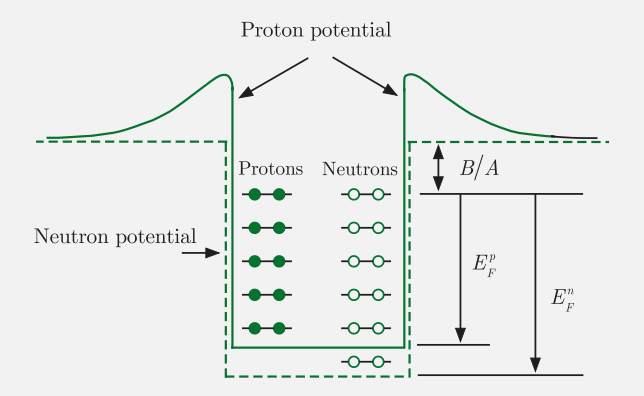
\includegraphics[width = .55\textwidth]{Fermi-Gas_model.png}
    \caption{Visual representation of the Fermi-Gas model}
\end{figure}
    \label{fig: Fermi-Gas_model}
\end{itemize}

\subsection{Shell Model \cref{fig: shell_model_energy_levels}}
\begin{itemize}
    \item A single particle model. Takes inspiration from the shell structure of the atom. 
    \item Explains the shell structure and properties of nuclei. Explains the magic numbers 
    \item The model assumes the particles do not interact. They are affected by a radial central spherical potential created by all the nucleons. It is therefore easier to estimate the movement of any single nucleon. 
    \item Nuclei with magic numbers are more stable. The magic numbers for protons are 2, 8, 20, 28, 50, 82. The magic numbers for neutrons are 2, 8, 20, 28, 50, 82, 126.
    \item Double magic nuclei are nuclei with magic numbers for both protons and neutrons.
    \item Instead of just having the nucleons pair up as in the Fermi-Gas model, the nucleons are arranged in shells.
    \item Each shell has a maximum number of nucleons.
    \item When certain magic number are reached, the separation energy is higher. They are therefore more stable.
    \item The electric quadrupole moment is the lowest for nuclei with magic numbers. This hints at them having a spherical shape, which is the most stable shape.
    \item Odd-Odd (Z-P) nuclei have only 4 stable isotopes. 
    \item Odd-Even nuclei have 50 stable isotopes.
    \item Even-Odd nuclei have 53 stable isotopes.
    \item Even-Even nuclei have 165 stable isotopes.
    
    \begin{figure}[h!]
    \centering
    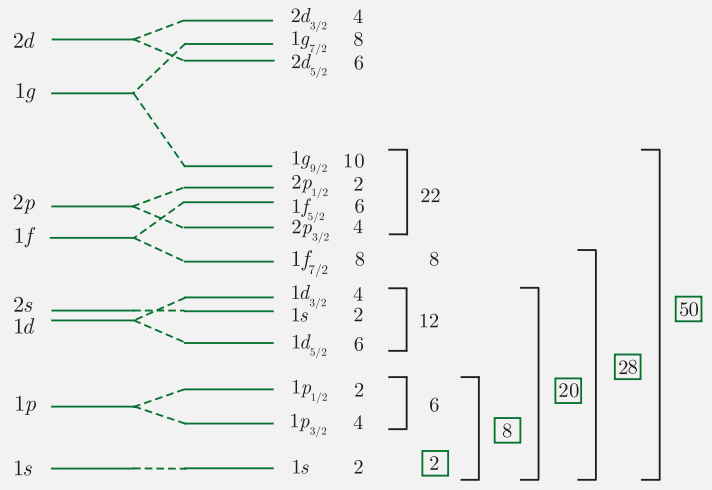
\includegraphics[width = .75\textwidth]{shell_model_energy_levels.png}
    \caption{Lowest energy levels for nucleons with their spin-orbit term.}
    \label{fig: shell_model_energy_levels}
    \end{figure}
    
\end{itemize}

\subsubsection{Simplifying the Complex System to a Simple Model \cref{fig: central_pot_simplification}}
\begin{figure}[h!]
\centering
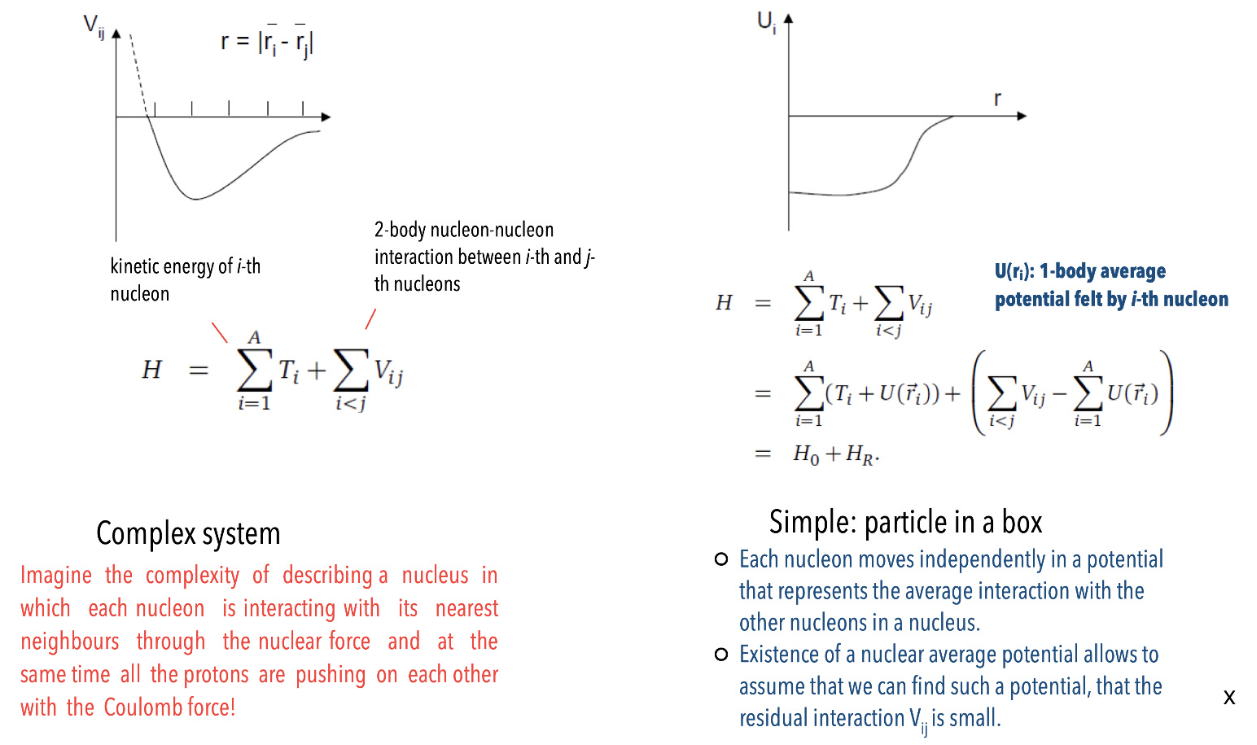
\includegraphics[width = .75\textwidth]{central_pot_simplification.png}
\caption{The transition from a complex system where all the particles interact, to a simple model where the nucleons are affected by a radial central spherical potential.}
\label{fig: central_pot_simplification}
\end{figure}


\subsubsection{Finding the Hamiltonian}
\begin{itemize}
    \item The system gets complex fast, when we have multiple unpaired nucleons. The Hamiltonian is then given by:
    \begin{equation}
      H = H_0 + H_{\text{res}}
    \end{equation}
    where $H_0$ is the Hamiltonian for the system with paired nucleons, and $H_{\text{res}}$ is the residual Hamiltonian for the unpaired nucleons. 
    \item To find the Hamiltonian we need the potential $U(r)$ and finally reproduce the magic numbers. 
\end{itemize} %# 12
\section{Relativistic Kinematics}
The conversion from one reference frame to another is done by the linear Lorentz transformation. The Lorentz transformation is given by \cref{eq: Lorentz_transformation} where $β = v / c$ and $γ 1 / \sqrt{1 - β^2}$. 
\begin{equation}\label{eq: Lorentz_transformation}
    \begin{pmatrix*}[r]
     ct \\
     x \\
     y \\
     z 
    \end{pmatrix*}' = 
    \begin{pmatrix*}[r]
     γ & 0 & 0 & -γβ \\
     0 & 1 & 0 & 0 \\
     0 & 0 & 1 & 0 \\
     -γβ & 0 & 0 & γ 
    \end{pmatrix*} 
    \begin{pmatrix*}[r]
     ct \\
     x \\
     y \\
     z 
    \end{pmatrix*} \ , \ 
    \begin{pmatrix*}[r]
     E / c \\
     p_x \\
     p_y \\
     p_z 
    \end{pmatrix*}' = 
    \begin{pmatrix*}[r]
     γ & 0 & 0 & -γβ \\
     0 & 1 & 0 & 0 \\
     0 & 0 & 1 & 0 \\
     -γβ & 0 & 0 & γ
    \end{pmatrix*}
    \begin{pmatrix*}[r]
     E / c \\
     p_x \\
     p_y \\
     p_z
    \end{pmatrix*}
\end{equation}
\paragraph{Example:}
For a particle at rest in coordinate system $s$, we have $\vec{p} = 0$ and $E = mc^2$. From here we can derive the energy and momentum in the $s'$ system.
\begin{equation}
  p_{z}' = - \frac{γβE}{c} = -mγβc = -mvγ
\end{equation}
\begin{equation}
  E' / c = γE / c = ymc → E' = γmc^2
\end{equation}
In this case we have $p'_{\perp} = p_{\perp}$, as the transformation is in the z-direction.

\subsection{Four-Vectors}
\begin{align}
    \vec{A} &= (A_0, a_x, a_y, a_z) \\
    \vec{B} &= (B_0, b_x, b_y, b_z)
\end{align}
\subsubsection{Dot product}
\begin{equation}
  \vec{A} ⋅ \vec{B} = A_0B_0 - a_xb_x - a_yb_y - a_zb_z ) \vec{A}^{T} η \vec{B}
\end{equation}
\begin{equation}
  η = 
    \begin{pmatrix*}[r]
    1 & 0 & 0 & 0 \\
    0 & -1 & 0 & 0 \\
    0 & 0 & -1 & 0 \\
    0 & 0 & 0 & -1
    \end{pmatrix*}
\end{equation}
\subsubsection{Dot product in different reference frames}
\begin{equation}
    \vec{A}' ⋅ \vec{B}' = 
    \begin{pmatrix*}[r]
    A_0 \\
    a_x \\
    a_y \\
    a_z
    \end{pmatrix*}^{T} 
    \begin{pmatrix*}[r]
    γ & 0 & 0 & -γβ \\
    0 & 1 & 0 & 0 \\
    0 & 0 & 1 & 0 \\
    -γβ & 0 & 0 & γ
    \end{pmatrix*} 
    \begin{pmatrix*}[r]
    1 & 0 & 0 & 0 \\
    0 & -1 & 0 & 0 \\
    0 & 0 & -1 & 0 \\
    0 & 0 & 0 & -1
    \end{pmatrix*}
    \begin{pmatrix*}[r]
    γ & 0 & 0 & -γβ \\
    0 & 1 & 0 & 0 \\
    0 & 0 & 1 & 0 \\
    -γβ & 0 & 0 & γ
    \end{pmatrix*}
    \begin{pmatrix*}[r]
    B_0 \\
    b_x \\
    b_y \\
    b_z \\
    \end{pmatrix*}
\end{equation}
Using the fact that $(ab)^{T} = b^{T} a^{T}$ we get:
\begin{equation}
    \vec{A}' ⋅ \vec{B}' = 
    \begin{pmatrix*}[r]
    A_0 \\
    a_x \\
    a_y \\
    a_z
    \end{pmatrix*}^{T}
    \begin{pmatrix*}[r]
    1 & 0 & 0 & 0 \\
    0 & -1 & 0 & 0 \\
    0 & 0 & -1 & 0 \\
    0 & 0 & 0 & -1
    \end{pmatrix*}
    \begin{pmatrix*}[r]
    B_0 \\
    b_x \\
    b_y \\
    b_z
    \end{pmatrix*} = \vec{A} ⋅ \vec{B}
\end{equation}
\subsubsection{Attributes Summary}
Consider the following attributes of the dot product of two four-vectors $\vec{A} = (ct,\vec{x})$ and $\vec{B} = (E / c , \vec{p})$. 
\begin{itemize}
    \item The dot product is invariant under Lorentz transformations. This means that the dot product is the same in all reference frames.
    \item $\vec{A}^2 = \vec{A} ⋅ \vec{A} = c^2t^2 - \left|\vec{x}\right|^2 = $ constant. 
    \item $\vec{B}^2 = E^2 / c^2 - \left|\vec{p}\right|^2 = $ constant. We define the invariant mass as mass in the rest frame. 
    \begin{equation}
      (Wc^2)^2 = E^2 - \left|\vec{p}\right|^2c^2
    \end{equation}
    If $\vec{p} = 0$ then $(Wc^2)^2 = E^2 = m^2c^{4}$, which makes $m = W$, the rest mass. 
    \item The invariant mass for a collation of particles is defined as the sum of the invariant masses of the particles.
    \begin{equation}
      (Wc^2)^ ≡ \left(∑_{i}^{} E_i\right)^2 - \left(∑_{i}^{} \left|\vec{p}_i\right|\right)^2c^2
    \end{equation}
    This allows us to measure the mass in any frame we find convenient. This allowed us to detect the Higgs boson, by looking at the invariant mass of the decay products which were photons. 
\end{itemize}

\subsection{Four-Momentum Transfer}
\begin{equation}
  Q^2 ≡ - \left(E - E'\right)^2 - \left(c \vec{p} - c \vec{p}'\right)^2 = - c^2 \left(\vec{P}_i - \vec{P}_f\right)^2
\end{equation}
Since $Q^2$ is dependant on the Lorenz invariant four-vectors, it is also Lorenz invariant. The probability amplitude for the Yukawa potential is therefore: 
\begin{equation}
  \mathcal{M} (Q^2) = \frac{-g^2 ℏ^2}{Q^2 + m^2 c^2}
\end{equation}
which is also Lorenz invariant.

\subsection{Invariant Mass of Virtual Photon}
Consider the following reaction:
\begin{equation}    
  e^{+} e^{-} → γ^{*} / Z^{*} → f \bar{f}
\end{equation}
We have a symmetric collider which $E_{b} → ← E_{b}$. The momentum of the virtual photon is 0. 
\begin{equation}
  \vec{p}_{γ}^{*} = 0 → Wc^2 = 2E_{b}
\end{equation}
We can then find the center mass energy:
\begin{equation}
  \sqrt{s} = Wc^2 = E_{\text{cm}} = 2E_{b}
\end{equation}

\subsubsection{Fixed-Target Experiment}
Consider a particle collision between a beam $b$, and a target $t$ at rest. How do we find the center mass energy?
\begin{equation}
  E_{b}^2 = m^2_{b}c^{4} + p^2_{b}c^{2} \quad , \quad  E_t = m_{t}c^{2}
\end{equation}
\begin{equation}
  (Wc^2)^2 = \left(∑_{i}^{} E_i\right)^2 - \left(∑_{i}^{} \left|\vec{p}_i\right|\right)^2c^2 = \left(E_{b} + m_tc^2\right)^2 - \left(\vec{p}_{b}c\right)^2
\end{equation}
If we let $c = 1$, we find $W$. 
\begin{equation}
  W = E_{\text{cm}} = \sqrt{m_{b}^2 + m_{t}^2 + 2E_{b}m_{t}}
\end{equation}
If the momentum is very large, we can neglect the masses of the particles so $E_{\text{cm}} = \sqrt{2m_{t}E_{b}}$. 

\section{Particle Accelerators}
\begin{itemize}
    \item Particles are accelerated by a voltage. This has a 1-1 correspondence with the energy for the electrons. Using a voltage of 1 MeV, we can accelerate electrons to an energy of 1 MeV.
    
\end{itemize}

\subsection{Linear Accelerators}
\begin{itemize}
    \item At high voltages, the field breaks down. Using an alternating current, we can avoid this.
    \item Radio frequency linear accelerators are used to accelerate particles to any energy, as the particle only feels the electric energy in the gaps. This is illustrated in \cref{fig: rad-freq_lin_acc}.
    \begin{figure}[h!]
    \centering
    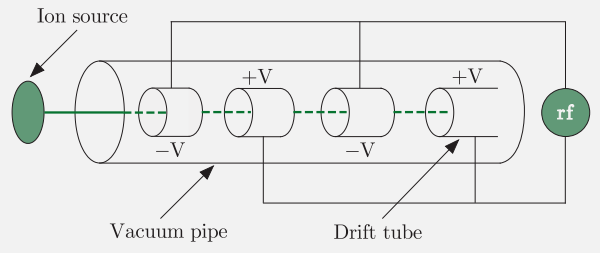
\includegraphics[width = .7\textwidth]{rad-freq_lin_acc.png}
    \caption{Illustration of a radio frequency linear accelerator. The voltages oscillate as the particles moves through the gaps. Only every second tube can be occupied. }
    \label{fig: rad-freq_lin_acc}
    \end{figure}
\end{itemize}

\subsection{Cyclotrons}
\begin{itemize}
    \item Using an oscillating current, the particle will start in the center, and spiral outwards. This is illustrated in \cref{fig: cyclotron}.
    \begin{figure}[h!]
    \centering
    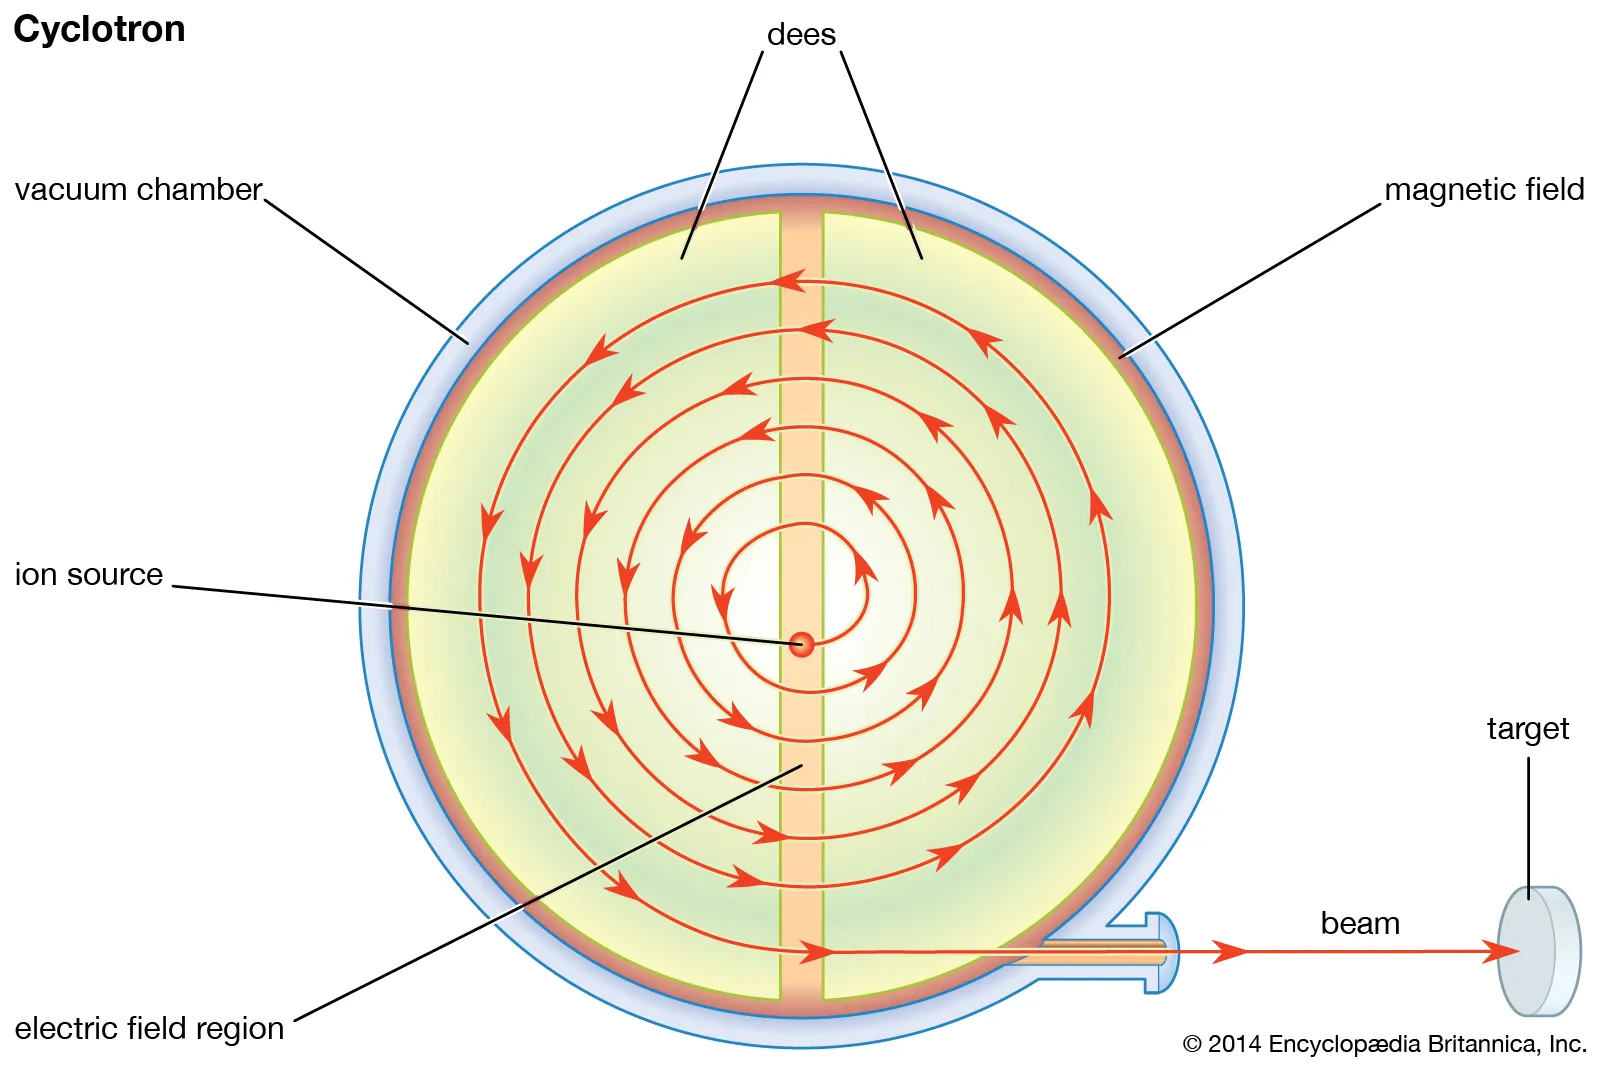
\includegraphics[width = .6\textwidth]{cyclotron.png}
    \caption{Illustration of a cyclotron. }
    \label{fig: cyclotron}
    \end{figure}
\end{itemize}

\subsection{Focusing of Particles}
\begin{itemize}
    \item Magnetic fields are used to focus the beam to a point. 
    \item Quadrupole magnets (4 poles) are often used. They work analogously to a optical lense. 
    \item The ability to focus the beam of some width $σ(s)$ is limited by the focusing properties $β(s)$ (the magnets) and how much each particle deviates from the beam $ε$. 
    \begin{equation}
      σ(s) = \sqrt{εβ(s)}
    \end{equation}
\end{itemize}

\subsection{Characteristics of Accelerators}
\begin{itemize}
    \item \textbf{Particle Type:} Protons, electrons, ions, etc.
    \item \textbf{Center of mass energy:} You need a certain amount of energy to create the different particles. You need $E_{\text{cm}} ≥ mc^2$. The wavelength of the particles is given by $λ = \frac{h}{p}$. You need a probe with an even smaller wavelength. 
    \item \textbf{Luminosity:} $R = \mathcal{L}σ$ where $\mathcal{L} = f n_1n_2 / 4πσ_xσ_y$. This shows the production rate $R$ needed. $n_1$ and $n_2$ are the number of particles, $σ_x$ and $σ_y$ are the transverse sizes of the beams. $f$ is the rate of collisions. 
\end{itemize}

\subsection{Large Hadron Collider (LHC)}
\begin{itemize}
    \item Circumference of 27 km.
    \item Four interaction points where the beams collide.
    \item Eight straight sections of 530m, leading to the IPs (intersection points). 
    \item 1200 superconducting dipole magnets are used to bend the beams.
    \item Can bunch $n = 1e 11$ protons with a collision frequency $f = 40$MHz. These are focused to a width of $σ = 20μ$m at the IP.
\end{itemize}

\subsection{Particle Types}
\begin{itemize}
    \item \textbf{Proton-Proton Colliders:} Initial state is unknown. There is a lot of background noise, which must be filtered.
    \item \textbf{Electron-Positron Colliders:} Initial state is known. The background noise is lower.
\end{itemize}


\subsection{Limitations}
\begin{itemize}
    \item \textbf{Circular proton-proton collider:} The strength of the magnetic fields limits the energy.  
    \item \textbf{Circular electron-positron collider:} The radiation loss makes it hard to reach high energies.
    \item \textbf{Linear electron-positron collider:} The width of the beam is a lot larger, making the luminosity requirements harder to reach.
\end{itemize}
 %# 13
\section{Neutrino Mixing Continued}
\begin{itemize}
    \item \textbf{Sterile Neutrinos}: A hypothetical fourth neutrino generation that does not interact with the weak force. It will therefore not be detected by the standard model detectors, but a gap in the number of neutrons after a reaction would point to its existence.
\end{itemize}

\subsection{Neutrino Mixing in Practice}
\begin{itemize}
    \item The different neutrinos interact with the electron through the $Z^{0}$-boson all the same. 
    \item The electron neutrino can also interact with the electron, through the $W^{-}$-boson. This would change the charge of each particle. 
\end{itemize}

\subsection{Quark Mixing}
\begin{itemize}
    \item Three generations of quarks: 
    \begin{enumerate}
        \item Up and Down $\displaystyle \begin{pmatrix*}[r]
         u \\
         d \\
        \end{pmatrix*}$
        \item Charm and Strange $\displaystyle \begin{pmatrix*}[r]
         c \\
         s \\
        \end{pmatrix*}$
        \item Top and Bottom $\displaystyle \begin{pmatrix*}[r]
         t \\
         b \\
        \end{pmatrix*}$
    \end{enumerate}
    \item The mass increases for each generation.
    \item Top-type quarks have a charge of $+\frac{2}{3}$, while bottom-type quarks have a charge of $-\frac{1}{3}$.
    \item All quarks are spin $\frac{1}{2}$ particles.
    \item No free quarks has been observer. We look at hadrons for information about quarks.
    \item High energy collisions of particle and anti-particles creates multiple jets of particles. This shows that there are multiple quarks in the hadrons.
    \item The top quark has such a short lifetime that it decays before it can form a hadron. It also has the greatest mass. 
    \item \textbf{Spectator Model}: A single quark involved in a hadron decay, assumes the other quarks are spectators and does not interact. 
    
    
\end{itemize}
\subsubsection{Quark Number \& Flavour Conservation}
\begin{itemize}
    \item Quark number for each flavour is conserved for electromagnetic and strong interactions. 
    \begin{equation}
      N_f ≡ N(f) - N(\bar{f}) \quad , \quad  f ∈ \left\{u, d, s, c, b, t\right\}
    \end{equation} 
    \item The flavour of the quarks are allowed to change through the weak interaction. This means the following interaction would be allowed:
    \begin{equation}
      c \overset{\underset{W^{+}}{}}{→} s u \bar{d} 
    \end{equation} 
    \item Baryon number is conserved in all interactions. The baryon number is defined as follows:
    \begin{equation}
      B ≡ N_q / 3 = \left(N(q) - N(\bar{q})\right) / 3
    \end{equation}
\end{itemize}

\subsection{Hadrons}
The most common hadrons are:
\begin{itemize}
    \item Baryons made up of three quarks. 
    \item Anti-baryons made up of three anti-quarks.
    \item Mesons made up of a quark and an anti-quark.
\end{itemize}

The strong force does not care about the flavour. The forces between the quarks are the same for all quarks. 

\subsection{Isospin}
\begin{itemize}
    \item The symmetry between the up and down quarks, with respect to the strong interaction. 
    \item Has nothing to do with regular spin. 
    \item The up and down sates are flavour states of the quarks. 
    \item The same can be used for protons and neutrons as two states of the nucleon. 
    \item The symmetry is just an approximation, as the masses and charge of the up and down quarks are not the same.
\end{itemize}

\subsubsection{Isospin Doublet}
\begin{itemize}
    \item The "light quark" and anti-light quark are noted as follows:
    \begin{equation}
        \begin{pmatrix*}[r]
        u \\
        d \\
        \end{pmatrix*} \quad , \quad \begin{pmatrix*}[r]
        \bar{u} \\
        -\bar{d} \\
        \end{pmatrix*}
    \end{equation} 
    \item In this framework, we can describe the nucleon as a state of the isospin doublet.
    \begin{equation}
        \begin{pmatrix*}[r]
        p \\
        n \\
        \end{pmatrix*} = 
        \begin{pmatrix*}[r]
         udu \\
         udd \\
        \end{pmatrix*} = 
        (ud) 
        \begin{pmatrix*}[r]
         u \\
         d \\
        \end{pmatrix*}
    \end{equation} 
    \item Example of the "Kaon":
    \begin{equation}
        \begin{pmatrix*}[r]
        K^{+} \\
        K^{0} \\
        \end{pmatrix*} = 
        \begin{pmatrix*}[r]
         u \bar{s} \\
         d \bar{s} \\
        \end{pmatrix*} =  
        \begin{pmatrix*}[r]
         u \\
         d \\
        \end{pmatrix*}
        (\bar{s})
    \end{equation} 
    \item Perfect isospin symmetry would mean that the mass of the proton and neutron would be the, just different charge. 
\end{itemize}

\subsection{Isospin Mathematics}
\begin{itemize}
    \item Same as with spin and angular momentum. 
    \begin{itemize}
        \item If $I = I_3$, we get $I_3 = -I, -I + 1, \ldots  , I - 1, I$
        \item If $I = 2 / 3$ we get $I_3 = -3 / 2, -1 / 2, 1 / 2, 3 / 2$
    \end{itemize}
    \item Addition works the same as for spin and angular momentum. 
    \begin{itemize}
        \item $I^{a} + I^{b} = \left|I^{a} - I^{b}\right|, \left|I^{a} - I^{b}\right| + 1, \ldots  ,I^{a} + I^{b}-1, I^{a} + I^{b}$
        \item If we have $I^{a} = I^{b} = 1$, we get: $1 + 1 = 0, 1, 2$
    \end{itemize} 
    \item For isospin conserving strong interactions we have the same sum-rule for the third $z$-component. 
    \begin{equation}
      I_3 = ∑_{i}^{} I_3^{i} \text{ where } I_3 (u, \overline{b}) = 1 / 2 \text{ and } I_3 (\bar{u}, d) = -1 / 2
    \end{equation}
\end{itemize}

\subsubsection{Isospin of Deuteron}
A deuteron is a proton and neutron. We need to use the sum rule, and third component of isospin to find the isospin of the deuteron.
\paragraph{Proton:}
\begin{equation}
  \ket{p, I, I_3} = \ket{\frac{1}{2}, \frac{1}{2}}
\end{equation}
\paragraph{Neutron:}
\begin{equation}
    \ket{n, I, I_3} = \ket{\frac{1}{2}, -\frac{1}{2}}
\end{equation}

\paragraph{Deuteron:}
\begin{equation}
  I_3(d) = I_3(p) + I_3(n) = \frac{1}{2} - \frac{1}{2} = 0
\end{equation}
We do not have enough information to find $I$. We do know that no other charge state with approximately the same mass, meaning the deuteron must be in a iso-singlet state of:
\begin{equation}
  \ket{I, I_3} = \ket{0, 0}
\end{equation}

\subsubsection{Isospin of a Pion and nucleon}
Given a final state with a pion $I = 1$ and a nucleon $I = 1 / 2$, what are the possible initial isospin states?

\paragraph{Solution 1:}
\begin{equation}
  \ket{I, I_3}  = \ket{\frac{1}{2}, ±\frac{1}{2}}
\end{equation}

\paragraph{Solution 2:}
\begin{equation}
\ket{I, I_3}  = \left\{\ket{\frac{3}{2}, ±\frac{3}{2}} , \ket{\frac{3}{2}, \pm \frac{1}{2}}\right\}
\end{equation}

\section{Spectroscopic Notation}
\begin{equation}
^{2S + 1}L_{J}
\end{equation}
where $S$ is the total spin of the continuans, $L$ is the total orbital angular momentum of the continuans. $J$ is the sum of the two, and can take many values. 
\begin{equation}    
  J = \vec{L} + \vec{S} → J = \left|L - S\right|, \left|L - S\right| + 1, \ldots  , \left|L + S - 1\right|,  \left|L + S\right|
\end{equation}

$L$ can take the following values:
\begin{table}[h!]
\begin{tabular}{ |c|c| }
\hline
L &Symbol \\ 
\hline
0 &S \\ 
1 &P \\ 
2 &D \\ 
3 &F \\ 
4 &G \\ 
\hline
\end{tabular}
\end{table}
$^{1}S_0$ means $J = S = L = 0$. 
 %# 14
\subsection{Use-case Example: Deuteron}
Deuteron $d$ has total spin $J = 1$, as each nucleon is half-spin particles. We also assume that the ground state has $L = 0$. The total state is therefore $^{3}S_1$. This predicts a magnetic dipole moment as the sum of the magnetic dipole moments of the proton and neutron. This is because we only take into account their intrinsic spins. This is close to what experiment show, but not quite. The reason for this discrepancy is that $L$ can be 2. This gives us the $^{3}D_1$ state. This explains the difference. For bound states, $L$ is only approximately a good quantum number. 

\section{Quark Model}
\subsection{Hadron Spectroscopy}
If we assume the following:
\begin{itemize}
    \item $L$ and $S$ are good quantum numbers. 
    \item Quarks have spin $1/2$.
    \item Mesons are $q \bar{q}$, baryons are $qqq$, with $q ∈ \left\{u, d, s, c, b\right\}$
    \item Lightest mesons states have $L = 0$. 
    \item Lightest baryon states have $L_{12} = L_3 = 0$
\end{itemize}
\subsubsection{Mesons}
\begin{itemize}
    \item Two possible spin states: $S = 0$ and $S = 1$.
    \item For $L = 0$ and $J = S$ we can have $^{1}S_0$ and $^{3}S_1$ states.
    \item This predicts two ground states with different spins. Things are more complicated with $L = 1$. 
    \item For $L = 1$ and $J = L - 1, \ldots  L +1$ if $S = 0$ or $J = L$ if $S = 0$. 
    \item For lighter mesons we have $L = 0$ and $S = 1$, for the lightest we have $S = 0$, as well. For heavier mesons we have $L = 1$. 
    \item The heavier ones have a shorter lifespan. 
\end{itemize}

\subsubsection{Baryons}
\begin{itemize}
    \item 3 spin-$1 / 2$ quarks so that $S = 1 / 2$ or $3 / 2$. 
    \item For $L = 0$ we have 2 states $^{2}S_{1 / 2}$ and $^{4}S_{3 / 2}$. 
    \item for $L = 1$ it again gets more complicated. We have 5 $P$-states and 6 $D$-states. 
    \item Light $S$-states include $p, n, Λ, Λ_{c}, Λ_{b}$. We expect to find heavier and more unstable states for $S = 3 / 2$. 
\end{itemize}

\subsection{Intrinsic Parity of Hadrons}
\begin{itemize}
    \item $P_{\text{meson}} = P_a P_{\bar{b}} (-1)^{L} = (-1)^{L+1}$. 
    \begin{itemize}
        \item Low-mass mesons with $L=0$ predicted to have $P = -1$, consistent with observations of $π$, $K$, $D$
    \end{itemize}
    \item $P_{\text{baryon}} = P_a P_b P_c (-1)^{L_{12} + L_3}$. 
    \item $P_{\text{anti-baryon}} = P_{\bar{a}} P_{\bar{b}} P_{\bar{c}} (-1)^{L_{12} + L_3} = (-1)^{L_{12} + L_3 + 1}$.
    \begin{itemize}
        \item Low bass baryons with $L_{12} = L_3 = 0$ predicted to have $P = +1$, with anti-baryons having $P = -1$.
    \end{itemize}
\end{itemize}

\subsection{Charge Conjugation (particle $\leftrightarrow$ anti-particle)}
\begin{itemize}
    \item The parity operator $\hat{C}$ changes particle to anti-particle and vice versa.
    \item Both $C$-parity and $P$-parity are conserved during strong and electromagnet interactions.
    \item Some particles, like the photon, are their own anti-particle. They are eigenstates of the operator $\hat{C}$.
    \item Other states have distinct anti-particles. They are not eigenstates of the operator $\hat{C}$.
    \item C-parity eigenstates can be constructed by particle-antiparticle paris that are symmetric or anti-symmetric under exchange of the particles $a \leftrightarrow \bar{a}$. This could be done as follows: 
    \begin{equation}
      \hat{C} \ket{a Ψ_1, \bar{a}Ψ_2} = \ket{\bar{a}Ψ_1, aΨ_2} = ± \ket{aΨ_1, \bar{a}Ψ_2}
    \end{equation} 
    \item An example could be the pion. 
    \begin{equation}
      \hat{C} \ket{π^{+} π^{-} ; L} = (-1)^{L} \ket{π^{-} π^{+} ; L}
    \end{equation}
\end{itemize}

\subsubsection{C-parity of pion $π^{0}$}
\begin{itemize}
    \item The pion often decays to two photons $\pi^{0} \rightarrow γγ$. The photons have their own C-parity, but as a unit they must have the same C-parity as the pion, $\hat{C} π^{0} = +1$. The question is, does the photons each have $C = +1$ or $C = -1$?
    \item As we never have observed a decay of the pion to three photons, we can conclude that the photons must have $C = -1$.
\end{itemize}

\subsubsection{C-parity of $η$}
\begin{itemize}
    \item Neutral spin-+ mesons with great mass of 558 MeV and spacial parity $\hat{P} η = -1$. 
    \item $B(η → γγ)$ happens $39\%$ of the time. We know the photons have $C = -1$, so the $η$ must have $C = +1$.
    \item $B(η → π^{0} π^{0} π^{0})$ happens $33\%$ of the time. The pions have $C = +1$, so the $η$ must have $C = -1$.
    \item $B(η → π^{+} π^{-} π^{0})$ happens $23\%$ of the time. Applying the C-parity operator to the pions as below:
    \begin{equation}
        \hat{C} \ket{π^{+}p_1, π^{-}p_2, π^{0}p_2} = \ket{π^{-}p_1, π^{+}p_2, π^{0}p_3} 
    \end{equation}
    This predicts that the momentum of the pions must be indistinguishable. 
    \item We can then predict why the probability of $B(η → π^{0} π^{0}) = 0\%$. It fulfills the conservation of C-parity, but not the spacial parity. One needs to check both attributes. 
\end{itemize}

\subsubsection{C-parity of Spin-1/2 Fermions}
General formula:
\begin{equation}
  \hat{C} \ket{f \bar{f}; J, L, S} = (-1)(-1)^{S + 1}(-1)^{L} \ket{f \bar{f}; J, L, S} = (-1)^{L + S} \ket{f \bar{f}; J, L, S}
\end{equation}
\begin{itemize}
    \item This comes from $(-1)^{L}$ from the space inversion. 
    \item $(-1)$ comes from the exchange of fermion-antifermion (QFT).
    \item The exchange of the spin wavefunction gives rise to the $(-1)^{S + 1}$ term.
\end{itemize}

\subsection{Quantum Numbers}
Important quantum numbers, where the subscripts stands for strangeness $s$, charm $c$, bottomness $b$, topness $t$ and quark $q$, respectively. They may or may not be conserved during weak interactions.:
\begin{itemize}
    \item $S = - (N_s - N_{\bar{s}})$
    \item $C = + (N_c - N_{\bar{c}})$
    \item $\tilde{B} = - (N_{b} - N_{\bar{b}})$
    \item $T = + (N_t - N_{\bar{t}})$
    \item $B ≡ N_q / 3 = \left(N_q - N_{\bar{q}}\right) / 2$
    \item Hypercharge $Y = B + S + C + \tilde{B} + T$
    \item Isospin $I_3 = \frac{1}{2}(N_u - N_d) - \frac{1}{2}(N_{\bar{u}} - N_{\bar{d}})$
    \item $I_3 = Q - Y / 2$, with $Q$ being the Coulomb charge.
    \item Full table of quark quantum numbers can be found in \cref{fig: quark_quantum_numbers}. The anti-quarks have the opposite quantum numbers, with the exception of Isospin $I$. $I_3$ is the opposite as well. 
    \item These numbers can be used as a basis for spanning out the possible states of quarks. 
\end{itemize}
\begin{figure}[h!]
\centering
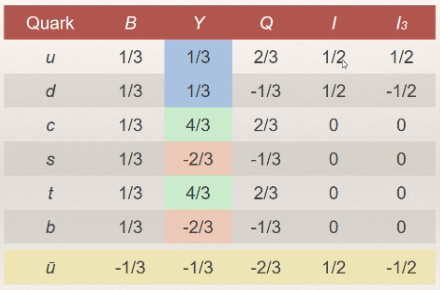
\includegraphics[width = .5\textwidth]{quark_quantum_numbers.png}
\caption{Table of quark quantum numbers.}
\label{fig: quark_quantum_numbers}
\end{figure}

\subsubsection{Hadrons With $C = \tilde{B} = T = 0$}
\begin{itemize}
    \item Isospin states: 
    \begin{itemize}
        \item $\frac{1}{2} + \frac{1}{2} = (0,1)$
        \item $\frac{1}{2} + \frac{1}{2} + \frac{1}{2} = (0,1) + \frac{1}{2} = \frac{1}{2}, \frac{1}{2}, \frac{3}{2}$
    \end{itemize}
    \item Table of isospin states can be found in \cref{fig: isospin_states}.
    \begin{figure}[h!]
    \centering
    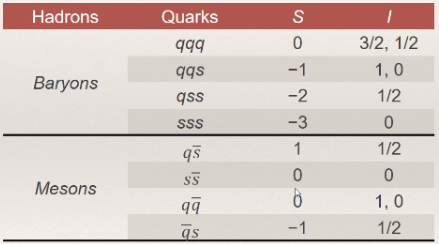
\includegraphics[width = .5\textwidth]{isospin_states.png}
    \caption{Table of isospin states.}
    \label{fig: isospin_states}
    \end{figure}
    
\end{itemize}

\paragraph{Example: $Σ^{+}$}
\begin{equation}
  K^{-} p → Σ^{+} π^{-}
\end{equation}
\begin{itemize}
    \item Looking at their quantum on the left-hand side we find that $S = -1$, $B = 1$, $C = \tilde{B} = T = 0$. The right-hand side has $S = 0$, $B = 0$, $C = \tilde{B} = T = 0$ and our $Σ^{+}$. For the quantities to be conserved we infer the values of the other $Σ^{+}$, which must be $S = -1$, $B = +1$, $C = \tilde{B} = T = 0$.
    \item Then we find the Isospin using $I_3 = Q - \frac{Y}{2}$ which gives $I_3 = 1$. We have two choices for $I$, either $0$ or $1$. As $I_3 = 1$, we must have $I = 1$ as well. This gives a $\ket{I, I_3} = \ket{1,1}$ state. 
    \item There must be two other charged members of the iso-triplet with $I_3 = 0, -1$, giving $Q = I_3 + Y / 2 = 0,-1$, as number of states are at least $N = 2 ⋅ I + 1$. We know from experiment this is $K^{0}$ and $K^{+}$. 
    \item The model predicted 3 states. There are no double charged $Σ^{--}$ or $Σ^{++}$ states. 
\end{itemize}

\subsubsection{Light Baryon Multiplets $L_{12} = L_3 = 0$ (\cref{fig: light_baryon_multiplets})}
\begin{figure}[h!]
\centering
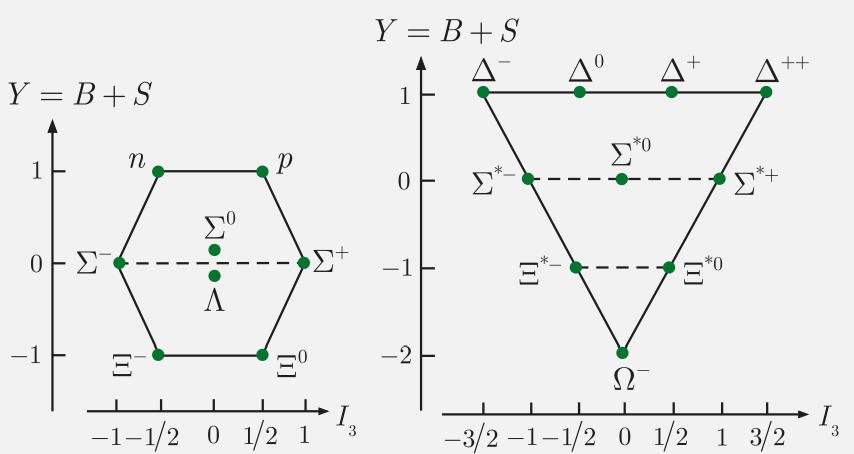
\includegraphics[width = .75\textwidth]{light_baryon_multiplets.png}
\caption{Different light baryon multiplets. Spin-1/2 particles to the left, and spin-3/2 particles to the right. On the bottom right, there should be a $Ω^{-}$.}
\label{fig: light_baryon_multiplets}
\end{figure}

\subsubsection{Light Mesons Nonets (\cref{fig: light_mesons_nonets,fig: quark_content})}





\begin{figure}[hb!]
\centering
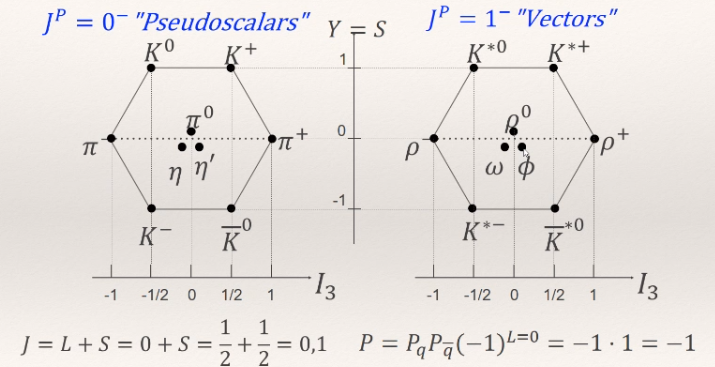
\includegraphics[width = .75\textwidth]{light_mesons_nonets.png}
\caption{Different light meson nonets. Pseudoscalar means that their wavefunction has some sign associated with it}
\label{fig: light_mesons_nonets}
\end{figure}

\begin{figure}[hb!]
\centering
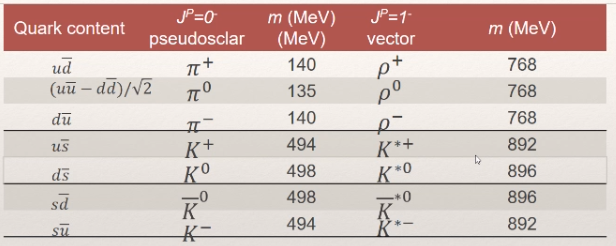
\includegraphics[width = .75\textwidth]{quark_content.png}
\caption{Quark content of different mesons and baryons. Some are unambiguously known, while others like $η$ and $\bar{η}$ are linear combinations of $u \bar{u}$, $d \bar{d}$ and $s \bar{s}$.}
\label{fig: quark_content}
\end{figure}



\subsection{Baryon Quark-Spin Wave Functions}
\begin{itemize}
    \item If we assume the wavefunctions $Ψ = ψ_{\text{space}}⋅ χ_{\text{spin}}$ of identical quarks are symmetric (while they are fermions), although this conflicts with the Pauli exclusion principle (for now). 
    \item As orbital angular momentum is 0, the the spin part must also be symmetric. This does not allow $S = 0$, as it would mean an anti-symmetric spin wavefunction. $S$ can only be $1$. 
    \item The only way to make $Δ^{++}(uuu)$, $Δ^{-}(ddd)$ and $Ω^{-}(sss)$, have symmetric spin is to have all three spins in parallel. This gives $J = 3 / 2$, and not $J = 1 / 2$
    \begin{itemize}
        \item For either $uud$, or $udd$, the two like quarks must be in $S = 1$, giving $↑_{a}↑_{a}↑_{b}$ or $↑_{a}↑_{a}↓_{b}$. The total $S = 1 + \frac{1}{2} = \frac{1}{2}, \frac{3}{2}$. 
        \item For protons and neutrons this gives $n,p → J = \frac{1}{2}$, and for $Δ^{+}, Δ^{0}$ we have $J = \frac{3}{2}$.
    \end{itemize}       
    \item For $uss$ and $dss$, the $ss$ must be in $S = 1$. When adding the third quark, the total $S = 1 + \frac{1}{2} = \frac{1}{2}, \frac{3}{2}$.
    \begin{itemize}
        \item For $Ξ^{-}$ and $Ξ^{0}$ with $J = 1 / 2$ and $Ξ^{*-}$ wnd $Ξ^{*0}$ with $J = 3 / 2$.
    \end{itemize}
    \item For $uus$ and $dds$, the non-$s$ must be in $S = 1$. When adding the third quark, the total $S = 1 + \frac{1}{2} = \frac{1}{2}, \frac{3}{2}$.
    \begin{itemize}
        \item For $Σ^{-}$ and $Σ^{+}$ with $J = 1 / 2$ and $Σ^{*-}$ and $Σ^{*+}$ with $J = 3 / 2$.
    \end{itemize} 
    \item For the $uds$-state we have $ud$ in $S = 1$, by isospin symmetry. the last $s$-quark gives $Σ^{0}$ with $J = 1 / 2$ and $Σ^{*0}$ with $J = 3 / 2$.
    \item An isospin-orthogonal $uds$ state has the $ud$ in $S = 0$. When adding the $s$ quark gives only one state of $S = 1 / 2$. This gives us $Λ$ with $J = 1 / 2$. Notice there is no excited state of $Λ$, as seen in \cref{fig: light_baryon_multiplets}.
\end{itemize}

 %# 14
\subsection{Heavy Quark-States (b,c)}
Patterns apply here as well. Using the quantum numbers as described in \cref{fig: quark_quantum_numbers}, we can find the quark content of the mesons in \cref{fig: heavy_baryon_nonets}

\begin{figure}[h!]
\centering
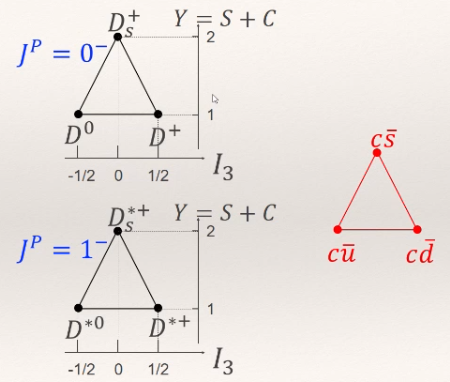
\includegraphics[width = .75\textwidth]{heavy_baryon_nonets.png}
\caption{Caption}
\label{fig: heavy_baryon_nonets}
\end{figure}


\subsubsection{Heavy Quarkonia}
\begin{itemize}
    \item Charmonium $c \bar{c}$ and Bottomonium $b \bar{b}$ are bound states of heavy quarks.
    \item They have the same quantum numbers as the virtual photon if $J^{PC} = 1 ^{--}$
    \item Process is shown in \cref{fig: heavy_quarkonia}
    \item \textbf{OZI rule}: Heavy quarks are suppressed in creatin/annihilation. This means they have long lifetimes. 
    \item For non-$J^{CP} = 1^{- - }$, we can still get heavier quarks, if there is emitted two photons, as they can have different quantum numbers.
    
    \begin{figure}[h!]
    \centering
    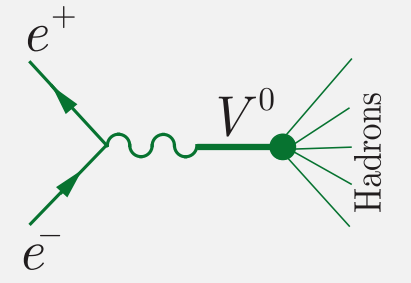
\includegraphics[width = .6\textwidth]{heavy_quarkonia.png}
    \caption{Production of heavy quarkonia in $e^+e^-$ annihilation.}
    \label{fig: heavy_quarkonia}
    \end{figure}
\end{itemize}

\paragraph{Potential:}
\begin{itemize}
    \item It was neither a radial or harmonic oscillator potential that could describe the heavy quarkonia.
    \item The solution was a linear term added to a radial term. This could also be a logarithmic term.
    \item $V(r) = - \frac{a}{r} + br$
    \item This points to a force between the quarks that increases as distance increases.
    \item The mass is then $M(q \bar{q}) = 2m_{q} + E(n,L)$, with $n$ being the principle quantum number.  
    \item The potential is flavour independent. 
\end{itemize}

\subsubsection{Exotic Hadrons}
\begin{itemize}
    \item tetraquarks and pentaquarks, etc. 
    \item Has spin 2. 
\end{itemize}

% \section{List of Concepts}
% \begin{itemize}
%     \item Leptons
%     \item Neutrinos
%     \item Quarks 
%     \item Hadrons 
%     \item Lepton universality 
%     \item Spectator model 
%     \item Yukawa potential
%     \item Range of force 
%     \item Amplitude 
%     \item Resonance
%     \item Breit-Wigner distribution 
%     \item Lifetime 
%     \item Decay rate 
%     \item Width 
%     \item Neutrino flavour eigenstates 
%     \item Neutrino mass eigenstates 
%     \item Neutrino mixing 
%     \item Neutrino oscillations
%     \item Sterile neutrino
%     \item Isospin 
%     \item Isospin multiplet
%     \item Hadron parity 
%     \item $Q, B, Y, I, S, C, \tilde{B}, T$
%     \item Baryon quark, spin wavefunction 
% \end{itemize}


\section{Quark Dynamics: The Strong Interaction}
\subsection{Quantum Chromodynamics (QCD)}
\begin{itemize}
    \item Quantitative theory of strong interactions 
    \item The gluon has zero mass. 
    \item The gluon couples to conserved color charges. 
    \item Static properties of hadrons, like when emitted from a quark are explained. 
    \item Dynamic properties of hadrons, like when scattered are explained.     
    \item Gluons have color charge, and can interact with it self or each other. This gives a three/four-gluon vertex which is not possible with photons.
    \item Bound states of gluons should exist. They are only predicted to exist. 
\end{itemize}

\subsubsection{Color Wavefunction}
\begin{itemize}
    \item By expanding the wavefunction with a color term, we can uphold the Pauli principle
    \begin{equation}
      Ψ = ψ_{\text{space}}  χ_{\text{spin}} χ_{\text{color}}
    \end{equation} 
    \item There are three possible colors, red, green, and blue, each associated with a conserved charge, called color hypercharge $Y^{C}$ and color isospin $I_3^{C}$. This is shown in \cref{fig: color_numbers}. 
    \item The sum of all three colors can bee seen as a white state. If only anti-quarks are present, we can see that as a black state. The net charge is zero either way. 
\end{itemize}

\begin{figure}[h!]
\centering
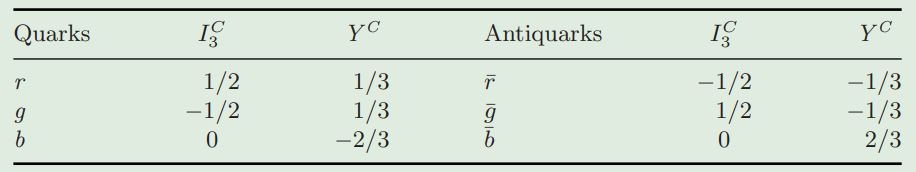
\includegraphics[width = \textwidth]{color_numbers.png}
\caption{Table of quark color and their respective charges. }
\label{fig: color_numbers}
\end{figure}
\subsubsection{Color Confiment}
\begin{itemize}
    \item Hadrons have no net color charge, meaning $I_3^{C} = Y^{C} = 0$. 
    \item The consequence of this is that no long-range gluon mediated strong force happens between nucleons. 
    \item Mesons consist of color-anticolor states. They are therefore "dark". 
    \item Baryons consist of three quarks, and are therefore "white".
    \item The color wavefunction is antisymmetric. 
    \begin{equation}
      χ_{\text{color}} = \frac{1}{\sqrt{6}} \left(r_1g_2b_3 - g_1r_2b_3 - b_1g_2r_3 + g_1b_2r_3 - r_1b_2g_3\right)
    \end{equation}
    \item Allowed numbers of quarks and anti-quarks are $(3q)^{p}(q \bar{q})^{n}$ where $p,n ≥ 0$
    \item Anti-baryons are also allowed, $(3q)^{p}(q \bar{q})^{n} → (3\bar{q})^{l}(3q)^{p}(q \bar{q})^{n}$ where $l,p,n ≥ 0$. 
\end{itemize}



\subsubsection{Gluon Color-States}
\begin{itemize}
    \item The gluon in tasked with keeping the color charge conserved. As seen in \cref{fig: gluon_color_conservation}, the gluon takes the color of the red quark, and passes it on to the blue quark. 
    \item Quarks have only color, but the gluon has color and anti-color. In this case it is $g = r \bar{b}$, as it neutralizes the total color charge and isospin. Summing up the $I_3^{C}$ and $Y^{C}$ of the quarks, gives the remaining value the gluon must have to have net zero charge.
    \item There are only 8 gluons, as the ninth does not interact with the quarks. This is called a non-interacting color singlet. 
\end{itemize}

\begin{figure}[h!]
\centering
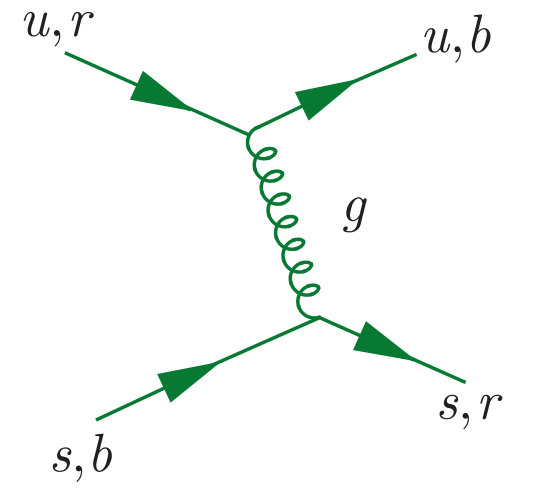
\includegraphics[width = .5\textwidth]{gluon_color_conservation.png}
\caption{Feynman diagram of gluon color conservation.}
\label{fig: gluon_color_conservation}
\end{figure}

\subsubsection{Confinemenet and Hadronization}
\begin{itemize}
    \item At small distances, the quark potential is proportional to $1 / r$. At larger distances, it becomes linear. 
    \item The slope of the linear potential is 1 GeV/fm. This is the same as the mass of the gluon, as the distance between quarks are about 1 fm.
    \item Supplying energy to increase the distance, spawns a jet of new hadrons. 
\end{itemize}

\subsubsection{Confiment and Asymptotic Freedom}
\begin{itemize}
    \item At short distances we have high momentum. Launching a high-energy quark into the hadron lets us look at short-range behavior.
\end{itemize}

\subsection{Running Coupling Constant}
\begin{itemize}
    \item At short distances, the coupling constant becomes small, and 1-gluon exchange is a good model. 
    \item At large distances or low energies, the coupling constant becomes large, and the potential increases with separation. This means gluons are confined inside hadrons. 
    \item The electromagnetic coupling constant increases with higher energies, but the strong coupling constant decreases.
\end{itemize}

\subsubsection{Running $α_s(μ)$ and OZI Rule}   
\begin{itemize}
    \item \textbf{OZI rule}: Creation or annihilation of heavy quarks pairs is suppressed with respect to light quarks. 
    \item Gluons connect the heavy-quark annihilation to the final state of hadrons. 
    \item The running coupling constant leads to reduced gluon coupling to heavy quark pairs, making them suppressed. 
    \item If a quark-antiquark decays, we need more than one gluon to conserve color. As the gluon has the same $C$-parity as the photon ($-1$), we need at least 3 gluons. This leads to suppression. 
\end{itemize}





 %# 16
\section{Shell Model Continued}
\subsection{Predicting the Magic Numbers}
\begin{itemize}
    \item Separate the wave function into a radial and angular part.
    \item Decide the form of the $U(r)$ potential. 
    \item Solve the Hamiltonian.
    \item Obtain single-particle energies $E_i$. This means the single-particle orbits. 
    \item The location of the single-particle orbits should be such that finally the correct magic numbers are reproduced. 
\end{itemize}

\subsubsection{Separating the Wave Function}
The angular dependance is independent of the radial distance from the central potential. The angular coordinates give the quantization conditions on $l$ and $m$, aka. $θ$ and $ϕ$
\begin{equation}
  Ψ_{nlm}(\vec{r}) = \frac{1}{r} R_{nl}(r) Y_{lm}(θ, ϕ)
\end{equation}
It is the radial part that gives the radial behavior and energies of the single-particle states. Solving the Schrödinger equation, we take into account the centrifugal force due to angular momentum.
\begin{equation}
  U = U(\vec{r}) + U_{\text{centrifugal}}
\end{equation}
\begin{equation}
  U_{\text{centrifugal}} = ∫ mw^2 r \ \mathrm{d}r = \frac{l(l+1) \hbar^2}{2m r^2}
\end{equation}
The solution of the Schrödinger equation for the radial part using this potential gives energy levels $E_{nl}$. The higher the $n$, the higher the energies. If equal $n$, the highest $l$ has the highest energy.

\subsubsection{Deciding the Form of the Potential}
\paragraph{Harmonic Oscillator / Square Well Potential:}

Solving the potential as an harmonic oscillator potential, gives energy levels $2, 8, 20, 40, 70$ and $112$. Only the the first three are actually magic numbers. We need some corrections. Using a square-well potential we can also produce some of the magic numbers, but not all. 

\paragraph{Degeneracy:}
The total number of states with the same energy is called the occupation number or total magnetic substance. This determines the total number of nucleons in each shell, and therefore the magic numbers. The total number is the number of possible spin-states and the number of possible angular momentum states. This gives: 
\begin{equation}
  m_{\text{total}} = m_s m_l = 2(2l+1)
\end{equation}
At the bottom, we have the $s$-state, with $l = 0 → m_l = 1$ and $m_s = 2$, giving $m_{\text{total}} = 2$, meaning only two nucleons can be in the $s$-state.

\paragraph{Wood-Saxon Potential:} 
This kind of potential works for the lowest magic numbers, but is still wrong. It adds a $l^2$ term which flattens the potential at the bottom. This is because it predicts larger orbits (having larger $l$) will be shifted towards the bottom. 

\paragraph{Wood-Saxon Potential with Spin-Orbit Term:}
The original Wood-Saxon potential is very close to a realistic model. Adding the spin-orbit term gives the correct magic numbers. 
\begin{equation}
  V(\vec{r}) = \frac{-V_0}{1 + \exp \left((r - R)/a\right)} - V_{ls}(r, \vec{l},\vec{s})
\end{equation}
When adding the spin-orbit term, we write the energy levels with a $j$-component, where $j = s + l$. The energy difference between the levels $ΔE_{ls}$ is given by:
\begin{equation}
    ΔE_{ls} = \frac{2l + 1}{2} ℏ^2 \left<V_{ls}\right>
\end{equation}
The higher the $l$, the lower the energy. This comes from $\left<V_{ls}\right>$ being negative. The total degeneracy is given by $2j + 1$. This is the new quantum number of interest as $l$ and $s$ can vary. 

\subsection{Predictions of the Shell Model}
\subsubsection{Ground State Spin-Parity of Even-Odd Nuclei}
If we want to find the ground-state spin-parity of $\ce{_{}^{15}\text{O}_{}}$, we know by filling up each layer of protons and neutrons separately, that the last nucleon must be in the $1p_{1 / 2}$ shell. This gives $I = 1 / 2$ and parity $π = (-1)^I = -1$. The parity is then $\mathbf{I}^{π}_{gs} = 1 / 2 ^{-}$. 

For $\ce{_{}^{}\text{17}_{}}$ we do the same, but here the last nucleon is in the $1d_{5 / 2}$ shell. This gives $I = 5 / 2$ with $π = +1$, resulting in $\mathbf{I}^{π}_{gs} = 5 / 2 ^{+}$. %# 17

We only take into account the last nucleon as the total parity of all paired nucleons is $+1$. No matter if the pair has both parity $+1$ or $-1$, the total parity is $+1$, as they are multiplied. 
\begin{equation}
  π = ∏_{i}^{A}  π_i = (-1)^{l_i}
\end{equation}

The Shell Model can predict many things, such as:
\begin{itemize}
    \item Ground state spin-parity 
    \item Excited states 
    \item Magnetic moments
    \item Electric moments 
\end{itemize}

\subsubsection{Ground State Spin-Parity of Odd-Odd Nuclei}
In the case of $\ce{_{49}^{110}\text{In}_{61}}$, we cannot get a single answer. The answer can be in the range of $\left|j_p - j_n\right| ≤ I ≤ j_p + j_n$. The parity is then $π = (-1)^{l_p} (-1)^{l_p}$. In this case, we have the proton at $1g_{9/2}$ with $j_p = 9/2$ and the neutron at $2d_{5/2}$ $j_n = 5/2$. This gives the possible values of $I ∈ \left\{2, 3, 4, 5, 6, 7\right\}$, with a parity of $π = (+)(+)$

\subsubsection{Ground State Spin-Parity of Even-Even Nuclei}
This is the easiest case. It is always $(+)$ as each nucleon has a partner with the same parity, and will therefore always give a positive parity. %# 18
\input{W12-1} %# 19
\input{W12-2} %# 20
\input{W13-1} %# 21
\input{W13-2} %# 22
\section{Jets: Quarks and Gluons}
Collisions of high energy particles with hadrons, produce jets of new hadrons or other particles. 

\subsection{Evidence for 3 Quark Colors}
\begin{itemize}
    \item The ratio $R$ between the cross-sections of producing hadrons in $e^+e^-$ collisions, compared to the cross-section of producing muons, show how many quark colors are possible. 
    \begin{equation}
      R ≡ \frac{σ(e^+e^- → \text{hadrons})}{σ(e^+e^- → μ^+μ^-)}
    \end{equation}
    The cross-section for producing hadrons is the sum of the cross-sections for producing quark-antiquark pairs with an center-mass energy too high to be produced. We must also take into account the number of colors $N_c$. 
    \begin{equation}
      σ(e^+e^- → \text{hadrons}) = ∑_{f}^{} σ(q_f \bar{q}_f) = ∑_{f}^{} N_c e^2_{f} σ(e^+e^- → μ^+μ^-)
    \end{equation}
    \begin{equation}
      R_0 ≡ N_c (e^2_{u} + e^2_{d} + e^2_{s} + e^2_{c} + e^2_{b} + e^2_{t}) = \frac{11}{9}N_c 
    \end{equation}
    Adding the gluon radiation we make a small correction. 
    \begin{equation}
      R_{\text{theory}} = R_0 \left(1 + \frac{α_s}{π}\right)
    \end{equation}
    \item The experimental values show that $N_c$ must be 3.
\end{itemize}


\subsection{Di-jet Production at $p p$ (\cref{fig: di-jet_production})}
\begin{figure}[h!]
\centering
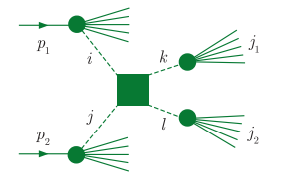
\includegraphics[width = .45\textwidth]{di-jet_production.png}
\caption{Dominant mechanism for di-jet production in $pp$ collisions.}
\label{fig: di-jet_production}
\end{figure}


\subsubsection{Rapidity}
Useful as $y_1 - y_2$ is lorentz invariant. 
\begin{equation}
  y = \frac{1}{2} \ln \left(\frac{E + p_z}{E - p_z}\right)
\end{equation}
\subsubsection{Pseudorapidity}
Practical high-energy approximation when you do not know everything about all particles. 
\begin{equation}
  η = -\ln \left(\tan \left(\frac{θ}{2}\right)\right)
\end{equation}

\subsubsection{Transverse Momentum}
When looking at collisions, we expect the transverse momentum to be zero. If this is not the case, it means some particle we did not detect, has taken some of the momentum.

\subsection{Current and Constituent Quarks}
\begin{itemize}
  \item The static quark model of hadrons consider them just staying still. 
  \item QCD is a dynamic theory, where quarks move at relativistic speeds, which affects their interactions with the gluons. 
  \item The masses of the quarks depends on their environment and what model is being used. Just as the coupling constants, they too run. 
  \item The mass of the proton comes from the interactions between the quarks through the strong force. The Higgs interataction contributes far less. 
\end{itemize}


\section{Weak Interactions and Electroweak Unification}
\begin{itemize}
  \item Untill 1973, we had only observed charged weak interactions, through the $W^{\pm}$-boson. We had already unified the electromagnetic and weak interactions (electroweak interactions) since the 1960s.
  \item It was nearly impossible to create a model with only the $W^{\pm}$-boson and the photon.
  \item The Brout-Englert-Higgs (BEH) predicted a neutral, heavy boson, the $Z^0$-boson.
  \item The neutral interactions were predicted to be found 1/3 as often as the charged interactions, which was later observed. 
\end{itemize}

\subsection{Low and High Energy Weak Interactions}
\begin{itemize}
  \item The invariant amplitude for Yukawa potential:
  \begin{equation}
    \mathcal{M} = \frac{g^2ℏ^2}{Q^2 - M^2c^2}
  \end{equation}
  shows that when momentum transfer $Q^2$ goes to zero, the great mass of the weak bosons makes the amplitude small. 
  \item This is the reason why the weak force is short-ranged.
  \item At low energies, the electromagnetic and weak forces can be seen as separate. 
  \item At high energies, the contribution to the Yukawa potential is about the same, and the forces can be seen as one.
\end{itemize}

\subsection{Charged Weak Interactions}
\subsubsection{Basic Principles}
\begin{itemize}
  \item \textbf{Lepton Universality}: The weak interactions are the same for all flavours.
  \item \textbf{Lepton-Quark Symmetry}: The coupling of the $W^{\pm}$ to leptons and all quarks are the same.
  \item \textbf{Quark Mixing}: The quark eigenstates (') are linear combinations of mass/strong-force eigenstates. 
  \begin{equation}\label{eq: quark_mixing}
    \begin{pmatrix}
      d' \\ s' \\ b'
    \end{pmatrix}
    = 
    \begin{pmatrix}
      V_{ud} & V_{us} & V_{ub} \\
      V_{cd} & V_{cs} & V_{cb} \\
      V_{td} & V_{ts} & V_{tb}
    \end{pmatrix}
    \begin{pmatrix}
      d \\ s \\ b
    \end{pmatrix}
  \end{equation}
\end{itemize}

\subsection{Quark Mixing}
\begin{itemize}
  \item Pions decay relatively slow via $π^{+} → μ^{+} ν_{μ}$
  \item This is the same as $u \bar{d} → μ^{+} ν_{μ}$ or $u \bar{d} → W^{+} → μ^{+} ν_{μ}$. 
  \item Kaons decay, with a long lifetime as well via $K^{+} →  μ^{+} ν_{μ}$. As a kaon is $u \bar{s}$ which is neither $u \bar{d}$ nor $c\bar{s}$, this means there must be some mixing. We can hypothesize that the weak and strong eigenstates of the quarks are not necessarily the same. 
  \item Using the same mixing hypothesis as for neutrino mixing, we believe mass eigenstates are mixtures of flavour eigenstates. 
  \begin{equation}
    \begin{pmatrix*}[r]
     d' \\
     s' \\
    \end{pmatrix*}  = 
    \begin{pmatrix*}[r]
      \cos θ_c & \sin θ_c \\
      -\sin θ_c & \cos θ_c \\
    \end{pmatrix*}
    \begin{pmatrix*}[r]
      d \\
      s \\
    \end{pmatrix*} = 
    \begin{pmatrix*}[r]
     V_{ud} & V_{us} \\
     V_{cd} & V_{cs} \\
    \end{pmatrix*} 
    \begin{pmatrix*}[r]
      d \\
      s \\  
    \end{pmatrix*}
  \end{equation}
\end{itemize}
\subsubsection{Examples}
$θ_{c}$ is the Cabibbo angle.
\paragraph{Pion}
\begin{equation}
u \bar{d}' = W^{+} → μ^{+} ν_{μ}
\end{equation}
\begin{equation}
  d' = d \cos θ_c + s \sin θ_c
\end{equation}
\begin{equation}
  u \bar{d} = W^{+} → μ^{+} ν_{μ}
\end{equation}
\paragraph{Kaon}
\begin{equation}
  u \bar{s}' → W^{+} → μ^{+} ν_{μ}
\end{equation}
\begin{equation}
  s' = -d \sin θ_c + s \cos θ_c
\end{equation} %# 23
  \subsection{Leptonic $W^{\pm}$-decay}
  \begin{itemize}
    \item The decay width $Γ$ is proportional to the square of the matrix element $|M|^2$, which is proportional to the square of the coupling constant $g_{W}^2$.
    \item As $m_{W} ≫ m_e ≫ m_{ν_e}$, it is the most important energy. 
    \item The natural width has units of energy, and is given by $Γ(W^{-} → e^{-} \bar{ν}_e) ∝ g^2_{W}m_{W}c^2$ which approximates to $α_{W}20$ GeV $= 0.223$ GeV. This gives $α_{W} ≈ 1/238$. This is a lot smaller than $α_{\text{EM}} = 1/137$
  \end{itemize}
  
  
  \subsection{Cabibbo Suppression}
  \paragraph{Cabibbo allowed process:} Has a matrix element $\left|V_{f_1f_2}\right|^2$ as seen in the quark mixing matrix defined in \cref{eq: quark_mixing}, which is approximately 1. 
  \paragraph{Cabibbo suppressed process:} Has a matrix element $\left|V_{f_1f_2}\right|^2$ as defined in \cref{eq: quark_mixing}, which is much smaller than 1.

  The ratio between the Kaon and Pion decay as depicted in \cref{fig: kaon_pion_decay} has a width ratio proportional to their couplings. We know from the linear combinations of the strange and down quarks that we get the following couplings:
  \begin{equation}
    d' = d \cos θ_c + s \sin θ_c → g_{ud} = q_{W}\cos θ_c
  \end{equation}
  \begin{equation}
    s' = -d \sin θ_c + s \cos θ_c → g_{us} = q_{W}\sin θ_c
  \end{equation}
  \begin{equation}
    \frac{Γ(K^{-} → μ^{-} \bar{ν}_{μ})}{Γ(π^{-} → μ^{-} \bar{ν}_{μ})} = \frac{g^2_{us}}{g^2_{ud}} = \tan^2 θ_c
  \end{equation}

\begin{figure}[h!]
\centering
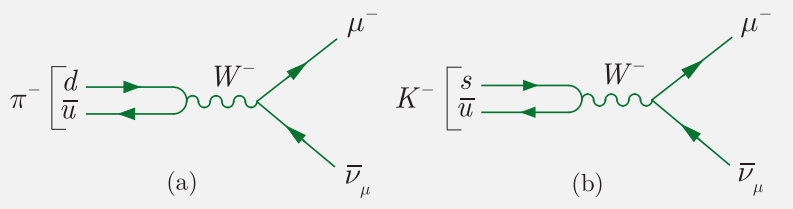
\includegraphics[width = .8\textwidth]{kaon_pion_decay.png}
\caption{Pion (a) and Kaon (b) decay through a charged weak interaction.}
\label{fig: kaon_pion_decay}
\end{figure}


\subsection{Charm Decays}   
\begin{itemize}
    \item From experiment we know $θ_{c} \approx 13 ^∘$
    \item As $\cos ^2 θ_c \approx 1$ and $\sin ^2 θ_c \approx 0$, we can roughly say that $d' \approx d$ and $s' \approx s$
    \item As a result of lepton-quark symmetry, we get: 
    \begin{itemize}
        \item $W^{+} → c \bar{s}$ and $W^{-} → u \bar{d}$ being \textbf{Cabibbo allowed}
        \item $W^{+} → c \bar{d}$ and $W^{-} → u \bar{s}$ being \textbf{Cabibbo suppressed}
    \end{itemize}
\end{itemize}

\subsubsection{Charmed Hadron Decays}
Given that $c → s'W^{+}$ we can expand that to $s'W^{+} = s \cos θ_c W^{+} - d \sin θ_c W^{+}$. Using the approximations from above, we can say that the charmed quark almost always decays into a strange quark.

\subsection{Selection Rules for Charged Weak Decays}
\subsubsection{Selection rules applied to hadronic part of charged weak decays}
\begin{itemize}
    \item The rules are derived from experiment. The capital letters denote if a quark is an up (U) or down (D) type quark. 
    \item \textbf{Semi-leptonic}: $D → W^{-} U$ or $\bar{U} → W^{-} \bar{D}$ followed by $W^{-} →  l^{-} \bar{ν}_l$
    \item Both of these have $ΔQ = +1$ to balance the charge of $W^{-}$. 
    \item We can have $d → W^{-} u$ or $\bar{u} → W^{-} \bar{d}$ which gives $ΔS = 0$
    \item We can also have $s → W^{-}u$ or $\bar{u} →  W^{-} \bar{s}$
\end{itemize}

\subsubsection{Semi-Leptonic Charged Weak Decays (\cref{fig: semi-leptonic_charged_weak_decays})} 
\begin{itemize}
    % \item
    \parbox[t]{\dimexpr\textwidth-\leftmargin}{
    \vspace{-7.5mm}
    \begin{wrapfigure}{R}{0.4\textwidth}
    \vspace{-5mm}
    \centering
    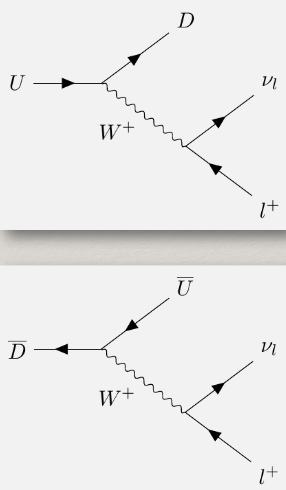
\includegraphics[width = .25\textwidth]{semi-leptonic_charged_weak_decays.png}
    \caption{}
    \label{fig: semi-leptonic_charged_weak_decays}
  \end{wrapfigure}
  
  \item $\bar{D} → W^{+} \bar{U}$ or $U → W^{+} D$ followed by $W^{+} → l^{+} ν_l$
  \item Both are $ΔQ = -1$ to balance the charge of $W^{+}$
  \item We can have $\bar{d} → W^{+} \bar{u}$ or $u → W^{+} d$ which gives $ΔS = 0$
  \item We can also have $\bar{s} → W^{+} \bar{u}$ or $u → W^{+} s$ which gives $ΔS = -1$
  \item In total we have $ΔS = 0$ with $ΔQ = ±1$ and $ΔS = ΔQ = ±1$. 
    \item There is no $ΔS = ±2$    
    }
  \end{itemize}
  
  
\vspace{0.5mm}
\subsubsection{Fully Hadronic Charged Weak Decays (\cref{fig: fully_hadronic_charged_weak_decays})}
\begin{figure}[ht!]
    \centering
    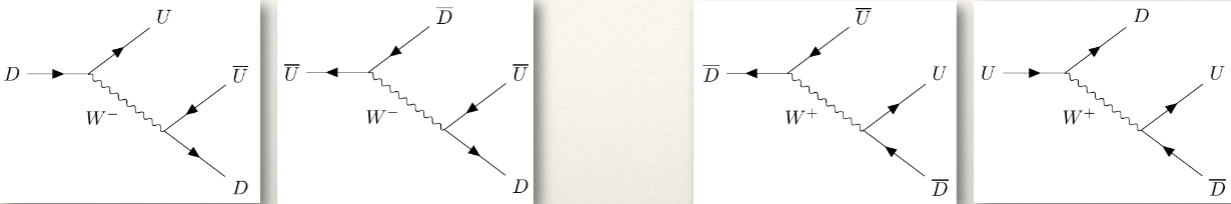
\includegraphics[width = .8\textwidth]{fully_hadronic_charged_weak_decays.png}
    \caption{Decay by the $W^{-}$ on the left, and by the $W^{+}$ on the right.}
    \label{fig: fully_hadronic_charged_weak_decays}
    \end{figure}

\begin{itemize} 
  \item Looking at the left side of \cref{fig: fully_hadronic_charged_weak_decays}:
  \begin{itemize}
    \item $ΔQ = 0$ by construction. 
    \item We can have $ΔS = 0$ or $ΔS = +1$ at the let vertices. 
    \item At the right vertices we can have $ΔS = 0$ or $ΔS = -1$. 
    \item All together we can have $ΔS = 0$ or $ΔS = ±1$
  \end{itemize}
  \item Looking at the right side of \cref{fig: fully_hadronic_charged_weak_decays}:
  \begin{itemize}
    \item $ΔQ = 0$ by construction.
    \item At the left vertices we can have $ΔS = 0$ or $ΔS = -1$.
    \item At the right vertices we can have $ΔS = 0$ or $ΔS = +1$.
    \item All together we can have $ΔS = 0$ or $ΔS = ±1$
  \end{itemize}
\end{itemize}

\subsubsection{Summary}
\begin{itemize}
  \item Selection rules apply to hadronic parts of decay. 
  \item \textbf{Semi-leptonic}: $ΔS = 0$ and $ΔQ = ±1$ and $ΔS = ΔQ = ±1$
  \item \textbf{Fully Hadronic}: $ΔS = 0$ or $ΔS = ±1$ with $ΔQ = 0$
  \item There is no $ΔS = ±2$
  \item There is no $Δs = -ΔQ = ±1$
  \item The above is derived from allowed $W^{±}$ and $S(s) = -S(\bar{s}) = -1$
\end{itemize}

\subsubsection{Consequence of Selection Rules}
Hadrons with multiple unstable quarks that decay weakly, decay in cascades. This means that particles which comes as a product from a decay, can decay further.

\paragraph{Example:}
The $π^{0}$ decays into two photons almost instantly.
\begin{align}
  \begin{aligned}
  &Ω^{-}(sss) → &&\underset{↓}{Ξ}^0(uss) + π^{-}(\bar{u}d) \\ 
  %
   &&&\begin{aligned}
      Ξ^{0} (uss) → &\underset{↓}{Λ}^{0}(uds) + π^{0}(\bar{u}u)\\ 
    %
      &\begin{aligned}
        Λ^{0} (uds) → p(uud) 
      \end{aligned}\\
    %
    \end{aligned}\\ 
  %
   &+ π^{-}(\bar{u}d)
\end{aligned}
\end{align}

\subsection{Three Generations}
\begin{itemize}
  \item We apply the letpon-quark symmetry to all generations $\begin{pmatrix*}[r]
   U \\
   D \\
  \end{pmatrix*}$. 
  \item A first approximation matrix is given by:
  \begin{equation}
    \begin{pmatrix*}[r]
     d' \\
     s' \\
     b' \\
    \end{pmatrix*} = 
    \begin{pmatrix*}[r]
      \cos θ_c & \sin θ_c & 0 \\
      -\sin θ_c & \cos θ_c & 0 \\
      0 & 0 & 1 \\
    \end{pmatrix*} 
    \begin{pmatrix*}[r]
      d \\
      s \\
      b \\
    \end{pmatrix*} = 
    \begin{pmatrix*}[r]
     V_{ud} & V_{us} & V_{ub} \\
     V_{cd} & V_{cs} & V_{cb} \\
     V_{td} & V_{ts} & V_{tb} \\
    \end{pmatrix*}
  \end{equation}
  \item Since the top quark is much heavier than the down quark, one could think the bottom quark is stable, but it is not. $τ_b ≈ 10^{-12}$s. 
  \item From measurements we know $\left|V_{ub}\right|^2 = 1.55 ⋅ 10^{-5}$, and $\left|V_{cb}\right|^2 = 1.78 ⋅ 10^{-3}$.
  \item As $\left|V_{cb}\right|^2$ is so much larger than $\left|V_{ub}\right|^2$, we can say the the bottom quark decays into a charm quark almost always.
  \item This is only a first approximation. In actuality, the top quark can sometimes decay into down and strange quarks, as the matrix above implies is impossible. The bottom quark also has a short lifetime. It is not zero. 
  \item The top quark have such a short lifetime $τ_{t} = 4 ⋅ 10^{-25}$, that light can't travel the single femto meter required for bonding to occur. The light would use approximately $10^{-23}$s, in which the top quark has decayed. There exist no top quark hadrons. 
  \item On the second row, we see the charm quark does not decay into the bottom quark due to its smaller mass. As the angle $θ_{c}$ is small, it most often decays to a strange quark, instead of a down quark. 
  \item When multiple strange, charmed and bottom quarks are present, they decay in cascades.
\end{itemize}

\subsection{Part 1 Essentials}
\begin{itemize}
  \item Inderstand what is meant by lepton-universality, lepton-quark symmetry and quark mixing, for the charged weak interaction.
  \begin{itemize}
    \item Apply these to find approximate rations of decay widths and cross-sections. 
  \end{itemize}
  \item Be able to sketch the main features of the quark-mixing matrix. 
  \begin{itemize}
    \item How does this influence quark and hadron decays?
  \end{itemize} 
  \item Be able to explain the origin of the "selection rules" for charged weak decays of hadrons. 
  \begin{itemize}
    \item Selection rules are one of the few things worth memorizing. Especially strangeness $Δs ∈ \left\{-1,0,1\right\}$
  \end{itemize}
\end{itemize}

\subsection{Electroweak Unification and the Higgs boson}
\subsubsection{Gauge Invariance}
\paragraph{Definition:} Gauge invariance means that the laws of physics behave the same way no  matter how you measure something. An example would be how the phase of a wavefunction $ψ = ψ_0e^{iθ}$ does to change the probability density $|ψ|^2 = |ψ_0|^2$. 

\textbf{It is not a symmetry of nature, but a redundancy in the description of nature.}

\begin{itemize}
  \item \textbf{Gauge invariance} and spontaneous symmetry breaking are the two main principles of the electroweak theory.
  \item \textbf{Gauge principle}: Propose a gauge (phase) transformation of the wavefunction and add an interaction so that the gauge remains unobservable. 
\end{itemize}

\paragraph{Gauge Invariance and EM}
  Fields in EM: 
  \begin{equation}
  \vec{B} = \vec{∇} × \vec{A} \quad , \quad  \vec{E} = - \vec{∇}ϕ - \frac{1}{c}\frac{∂ \vec{A}}{∂ t}
  \end{equation}

  Gauge transformations of potential $ϕ$ and vector potential 
  \begin{equation}
    \vec{A} (ϕ, \vec{A}) → (ϕ, \vec{A})' →  \left(ϕ - \frac{1}{c}\frac{∂ α}{∂ t}, \vec{A} + \vec{∇}α\right)    
  \end{equation}
  where $α(t, \vec{h})$ is a doubly differentiable function.

  This gives 
  \begin{equation}
    \vec{B}' = \vec{∇} × \vec{A}' = \vec{∇} × \left(\vec{A} + \vec{∇}α\right) = \vec{∇} × \vec{A} + \vec{∇} × \vec{∇}α 
  \end{equation}
  The last cross product gives: 
  \begin{equation}
    \vec{∇} × \vec{∇}α ≡ 0
  \end{equation}
  as it is the curl of a scalar field. This means $\vec{B} = \vec{B}' = \vec{∇} × \vec{A}$
  Adding this back into the electric field we get:
  \begin{equation}
    \vec{E}' = - \vec{∇} \left(ϕ - \frac{1}{c}\frac{∂ α}{∂ t}\right) - \frac{1}{c}\frac{∂}{∂ t} \left(\vec{A} + \vec{∇}α\right) = - \vec{∇}ϕ - \frac{1}{c}\frac{∂ \vec{A}}{∂ t} + \frac{1}{c}\left( \underbrace{\vec{∇} \frac{∂ α}{∂ t} - \frac{∂}{∂ t} \vec{∇}α}_{0}\right)
  \end{equation}
  \begin{equation}
    \vec{E}' = - \vec{∇}ϕ - \frac{1}{c}\frac{∂ \vec{A}}{∂ t} = \vec{E}
  \end{equation}
  This shows that the electric and magnetic field are unaffected by the gauge transformation $(ϕ,\vec{A}) → (ϕ,\vec{A})'$. With gauge symmetry we get the conservation of charge.

  \subsubsection{Statndard Model Gauge Interactions}
  \begin{itemize}
    \item Introduce locale gauge (phase) transformation. 
    \item \textbf{QED:} $ψ → e^{-iqα(\vec{x})}ψ$, gives a photon. 
    \item \textbf{QCD:} $ψ → e^{-iqα(\vec{x}) ⋅ T_{a}}ψ$, with $T_a = $ 8 color matrices (3X3) gives 8 gluons.
    \item \textbf{Electroweak:} $ψ → e^{-ig'α(\vec{x}) ig \vec{τ} \vec{Λ}(\vec{x})}$ with $\vec{τ} = $3 Pauli matrices, $g'$ the coupling to weak hypercharge singlet ($B^{0}$) and $g$ the coupling to weak isospin triplet ($W^{± /0}$).
    \item The choice of gauge symmetry determines dynamics of the system. 
  \end{itemize}

  \subsubsection{Electoweak Unification/Mixing}
  \begin{itemize}
    \item \textbf{Mixing Hypothesis}: What if the basis of nature is not the $B^{0}$ and $W^{±}$-boson, but the photon and $Z^{0}$-boson?:
    \begin{equation}
      \begin{pmatrix*}[r]
        γ \\
        Z^{0} \\
      \end{pmatrix*} = 
      \begin{pmatrix*}[r]
        \cos θ_{W} & \sin θ_{W} \\
        -\sin θ_{W} & \cos θ_{W} \\
      \end{pmatrix*}
      \begin{pmatrix*}[r]
        B^{0} \\
        W^{±} \\
      \end{pmatrix*}
    \end{equation}
    \item The mixing angle $θ_{W}$ (Weinberg angle) is defined by $\cos θ_{W} ≡ m_{W} / m_{Z}$
    \item Unification condition: $e = g \sin θ_{W} = g' \cos θ_{W}$ with massless photon without any neutrino interactions. 
    \item Gauge symmetry removes divergence in the center mass energy $\sqrt{s}$ when adding the contribution from the photon and $Z^{0}$-boson.
    \item A divergence-free theory is a renormalizable theory. An important property. 
  \end{itemize}
  
\subsubsection{Other Predicitons}
\begin{itemize}
  \item There can be mathematical anomalies in as long as the sum of the lepton charges and  the number of colors charges times the sum of quark charges is zero. 
  \begin{equation}
    ∑_{l}^{} Q_l + 3 ∑_{q}^{} Q_q = 0
  \end{equation}
  \item The standard model can have more generations, but have been adapted to the three observed. 
  \item At low energies we get:
  \begin{equation}
    G_{W} ≡ G_{F} = \frac{(ℏc)^2 \sqrt{2}g^2_{W}}{m^2_{W}c^4}  \quad , \quad  G_{Z} = \frac{(ℏc)^2 \sqrt{2}g^2_{Z}}{m^2_{Z}c^4}
  \end{equation}
  With a ration:
  \begin{equation}
    \frac{G_{Z}}{G_{F}} = \frac{\sin ^2θ}{\cos ^2θ}\cos ^2θ = \sin ^2θ_{W} ≈ 0.21
  \end{equation}
  As the angle is so small, some conclude the $G_{Z} = G_{F}$.
  \item In experiment we get a ratio of $1/3$, which does not match with the theory of $\sin^4 θ_{W} ≈ 0.05$
\end{itemize}  %# 24
\section{Radioactive Decay}
\begin{figure}[ht!]
\centering
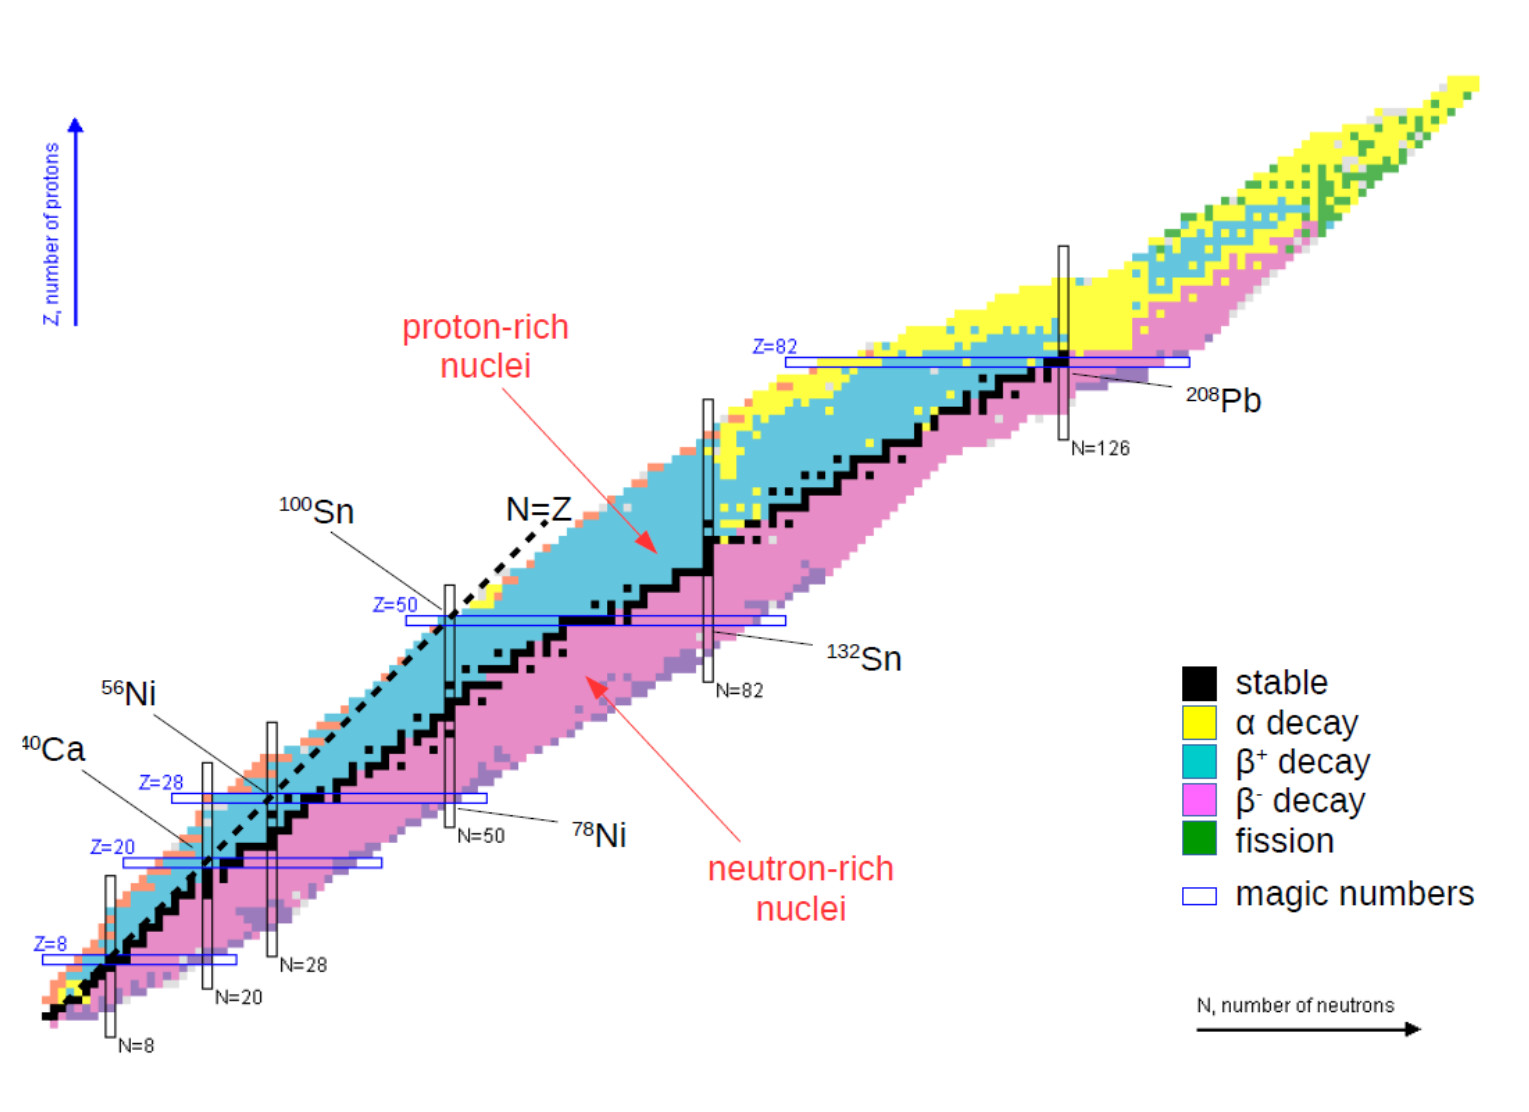
\includegraphics[width = .8\textwidth]{radioactive_nuclei_chart.png}
\caption{Chart of the nuclei and their decay modes.}
\label{fig: radioactive_nuclei_chart}
\end{figure}

\begin{itemize}
    \item Naturally occurring nuclei goes through a combination of $α$, $β$ and $γ$ decay.
    \item Spontaneous decays occur when the $Q$-value is positive 
    \begin{equation}
      Q = (M_i - M_f)c^2
    \end{equation}
    \item Artificially produced nuclei can also decay by spontaneous fission, neutron emission, proton emission and heavy iron emission in addition to the natural decay modes.
\end{itemize}

\subsection{Exponential Decay}
\subsubsection{The Law}
The number of radioactive nuclei $N(t)$ at time $t$ is given by the exponential decay law, where $λ$ is the decay constant. 
\begin{equation}
  N(t) = N_0 e^{-λt}
\end{equation}

\subsubsection{Half-Life}
The time it takes to reduce the intensity of radiation by half. 
\begin{equation}
  t_{1/2} = \frac{\ln 2}{λ} ≈ \frac{0.693}{λ}
\end{equation}

\subsubsection{Mean Lifetime}
The average time that a  nucleus is likely to survive before decaying. This is often referred to as the lifetime of the nucleus.
\begin{equation}
  τ = \frac{1}{λ}
\end{equation}

\subsubsection{Activity}
Activity is the number of decays per unit time. This is a lot more practical to work with, as it is easier to measure the number of decays in a given time period than the number of nuclei.
\begin{equation}
  A(t) = \frac{\mathrm{d}N(t)}{\mathrm{d}t} =  A_0 e^{-λt} \quad , \quad  A_0 = λN_0
\end{equation}

\paragraph{Units of Activity:} 
The unit of activity is the Becquerel (Bq). 
\begin{equation}
  1 \text{ Bq} = 1 \text{ decay/s}
\end{equation}
It is more common to use the Curie (Ci). 1 Ci i the activity of 1g of $\ce{_{}^{226}\text{Ra}_{}}$
\begin{equation}
  1 \text{ Ci} = 3.7 \times 10^{10} \text{ Bq}
\end{equation}

\paragraph{Important Note:}
Knowing the activity, does not tell you its lifetime or halflife and vice versa. Saying something is highly radioactive, does not tell you about the danger or the energy of the radiation.

\subsubsection{Measuring Short and Long Lifetimes and Activity}
\begin{itemize}
    \item After 10 half-lives, the activity is reduced to $1/1024$ of the original activity. We assume the activity is zero after 10 half-lives. 
    \item This means if the half-lifte is short (like 1 second), you have only 10 seconds to measure the activity.
    \item If the half life is very long (like 100 years), you will not live to measure the activity.
\end{itemize}

\subsubsection{When the Decay Law Fails}
If the parent nucleus decays into a daughter nucleus, which is also radioactive, the decay law fails as the number of children does not stay the same, they create grandchildren. 

\subsection{Decay Options}  
For isotopes which are able to decay in multiple ways, the total decay rate is the sum of the decay rates for each decay mode.
\begin{equation}
  λ_\text{tot} = ∑_{i}^{} λ_i = \frac{1}{τ_\text{tot}} = ∑_{i}^{} \frac{1}{τ_i}
\end{equation}

\subsection{Mixed Samples}
\begin{wrapfigure}{r}{0.4\textwidth}
\vspace{-6.5mm}
\centering
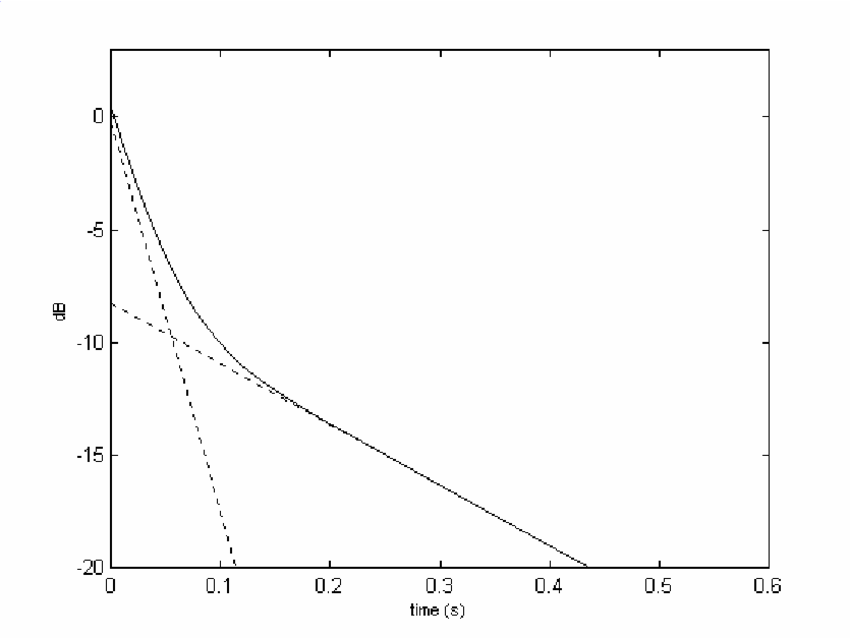
\includegraphics[width = .35\textwidth]{mixed_sample_decay.png}
\caption{Visualisation of the decay of a mixed sample. The y-axix is logarithmic.}
\label{fig: mixed_sample_decay}
\end{wrapfigure}
With more than one isotope in a sample, we can wait ten half-lives for the shortest lived isotope to decay, and then measure the activity of the remaining isotopes. This is the case for $\ce{}^{64}\text{Cu}_{}(12\text{h})$ and $\ce{}^{61}\text{Cu}_{}(3.4\text{h})$, which can't be separated chemically. Plotted out on a semi-log curve, we would still set a total decay curve looking logarithmic. If you wait until it becomes linear, you know you only have the decay of one isotope left. This is visualized in \cref{fig: mixed_sample_decay}.

\subsection{Types of Radioactive Decay}
\paragraph{$α$-Decay:}
Decaying of alpha particles ($\ce{_{}^{4}\text{H}_{}}$). This occurs when Radium decays to Radon. This has a half-life of about 1600 years.

\paragraph{$β$-Decay:} 
Split into two types, $β^-$ and $β^+$ decay. We also have electron capture.
\begin{itemize}
    \item $β^-$-Decay: A neutron decays into a proton, an electron and an electron antineutrino. This happens when $\ce{_{53}^{131}\text{I}_{78}}$ decays into $\ce{_{54}^{131}\text{Xe}_{77}}$. The half-life of which is 8 days.
    \item $β^+$-Decay: A proton decays into a neutron, a positron and an electron neutrino. A lone proton cannot decay, but a proton in a nucleus can. The half-life of a proton is $10^{34}$ years. An example ishw ne $\ce{_{13}^{25}\text{Al}_{12}}$ decays to $\ce{_{12}^{25}\text{Mg}_{13}}$, with a half-life of 7.2 seconds. 
    \item Electron Capture: A proton captures an electron and decays into a neutron and an electron-neutrino. An example is when $\ce{_{25}^{54}\text{Mn}_{29}}$ decays into $\ce{_{24}^{54}\text{Cr}_{30}}$ with a half-life of 312 days. Electron capture is more common in proton-rich nuclei with higher chance of $β^{+}$-decay. 
\end{itemize}

\paragraph{$γ$-Decay:}
When a nucleus is in an excited state, it can decay to a lower energy state by emitting a photon. The half-life can be anything from $1μ$s to minutes, to hours or even years. These are often called metastable states. Metastable states are noted with an $m$ like so: $\ce{_{Z}^{Am}\text{X}_{N}}$. For nuclear physics, one can consider nano-second half-lives as metastable. 


\subsubsection{Branching Ratios and Partial Half-Lives}
\begin{wrapfigure}{r}{0.5\textwidth}
\vspace{-4mm}
\centering
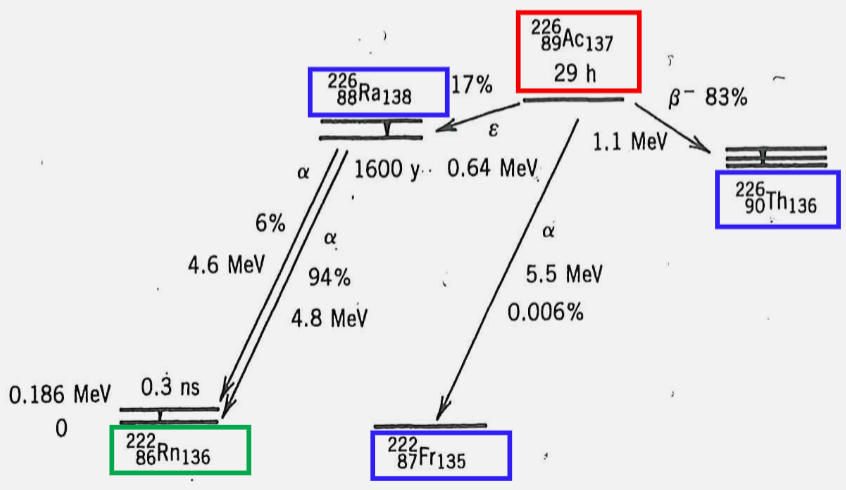
\includegraphics[width = .45\textwidth]{decay_branches.png}
\caption{Example of a parent (red) decaying into three different children (blue) by different modes. One of the children decays again into a grandchild (green).}
\label{fig: decay_branches}
\end{wrapfigure}
When a nucleus can decay in multiple ways, we get different branching ratios. The branching ratio is the fraction of decays that go through a specific decay mode. This is often referred to as the intensity of the decay modes. An example can be seen in \cref{fig: decay_branches}. 

To find the total half-life, we first use the total decay constant $λ_\text{tot}$, and then we can find the partial half-lives by. 
\begin{equation}
  λ_{\text{tot}} = \ln 2 / t_{1/2} ≈ 6.6 ⋅ 10^6 \text{s}^{-1}
\end{equation}
From this we find each decay constant as follows:
\begin{align}
  &λ_{β} = 0.83 λ_{\text{tot}}  = 5.5 ⋅ 10^6 \text{s}^{-1} \\
  &λ_{ε} = 0.17 λ_{\text{tot}}  = 1.1 ⋅ 10^6 \text{s}^{-1} \\
  &λ_{α} = 6 ⋅ 10^{-5} λ_{\text{tot}}  = 4.0 ⋅ 10^{-10} \text{s}^{-1}
\end{align}


And from here we easily find the partial half-lives.  
\begin{align}
  &t_{1/2,β} = \ln 2 / λ_{β} ≈ 1.3 ⋅ 10^{5} \text{s} ≈ 35 \text{h} \\
  &t_{1/2,ε} = \ln 2 / λ_{ε} ≈ 6.1 ⋅ 10^{5} \text{s} ≈ 170 \text{h} \\
  &t_{1/2,α} = \ln 2 / λ_{α} ≈ 1.7 ⋅ 10^{9} \text{s} ≈ 55 \text{y}
\end{align}
\subsubsection{Width-Lifetime Relation}
\paragraph{Stationary State:}
Does not decay. The energy is precisely defined with zero uncertainty. 
\begin{equation}
  ΔE = \sqrt{\langle E^2 \rangle - \langle E \rangle^2} = 0
\end{equation}
\begin{equation}
  ΔE Δt ≥ \frac{\hbar}{2}
\end{equation}

\paragraph{Non-Stationary State:}
Does eventually decay. The energy is not precisely defined, and has a finite uncertainty. A short lifetime means large decay and energy width, and vice versa. 
\begin{equation}
  ΔE = \sqrt{\langle E^2 \rangle - \langle E \rangle^2} ≠ 0
\end{equation}
\begin{equation}
  ΔE Δt ≥ \frac{\hbar}{2}
\end{equation}
\begin{equation}
  ΔE = Γ \quad , \quad  Δt = τ
\end{equation}
\begin{equation}
  τ ≈ \frac{\hbar}{Γ} = \frac{1}{λ}
\end{equation} %# 25
\subsection{Alpha Decay}
\begin{itemize}
    \item As seen in \cref{fig: radioactive_nuclei_chart}, heavier nuclei tend to decay by emitting an $\alpha$ particles, and are often referred to as $α$ emitters. 
    \item This is caused by the Coulomb force having a much longer range than the strong force. As nuclei grows large, they need more neutrons to stabilize the nucleus, but it can quickly become too much. 
    \item $α$ particles are the most tightly bound, and calculated to be the only way to decay with a positive Q-value, making it spontaneous. One could imagine just emitting a single proton, but the Q-value would be negative.
    \begin{equation}
      \ce{_{}^{232}\text{U}_{}} → \ce{_{}^{4}\text{He}_{}} + \ce{_{}^{228}\text{Th}_{}}
    \end{equation}
    \begin{equation}
      Q_{α} = M\left(\ce{_{}^{232}\text{U}_{}}\right) - \Big(M\left(\ce{_{}^{4}\text{He}_{}}\right) + M\left(\ce{_{}^{228}\text{Th}_{}}\right)\Big)c^2 = 5.41 \text{ MeV}
    \end{equation}
\end{itemize}

\subsubsection{Energetics of Alpha Decay}
We take the general case of:
\begin{equation}
  \ce{_{Z}^{A}\text{X}_{N}} → \ce{_{Z-2}^{A-4}\text{Y}_{N-2}} + α
\end{equation}
The we have energy conservation, where $T$ is the kinetic energy and $p$ is the momentum:
\begin{equation}
  m_{X}c^2 = m_{Y}c^2 + T_{Y} + m_{α}c^2 + T_{α}
\end{equation}
\begin{equation}
  \Big(\underbrace{m_{X} - \left(m_{Y} + m_{α}\right)}_{Q-\text{value}}\Big)c^2 = T_{Y} + T_{α}
\end{equation}
\begin{equation}
  Q = T_{Y} + T_{α}
\end{equation} 
As we assume the system is at rest, there should be no net momentum. We do not care about the sign. 
\begin{equation}
  p_{Y} = p_{α}   
\end{equation}
We get the kinetic energy of the $\alpha$ particle:
\begin{equation}
  T_{α} = \frac{Q}{1 + m_{α}/m_{Y}}
\end{equation}

This resembles the taylor expansion of $1/(1 + x)$:
\begin{equation}
  \frac{1}{1 + x} = 1 - x + x^2 - x^3 + \dots
\end{equation}
From this we get an approximation for the kinetic energy of the $\alpha$ particle from the Q-value. As it is easy to measure the momentum of the $α$ particle, we have a shortcut to the Q-value.
\begin{equation}
  T_{α} = Q\left(1 - \frac{m_{α}}{m_{Y}}\right) = Q\left(1 - \frac{4}{A}\right)\quad , \quad  m_{α} ≈ 4 \ , \ m_{Y} ≈ A
\end{equation}


\subsubsection{$Q$-value and Half-life}
\begin{itemize}
  \item The $Q$-value is closely related to the half-life of the decay.
  \item The greater the $Q$-value, the shorter the half-life. This makes sense as it is very energetically favorable to decay.
  \item Even-odd and odd-even $α$ emitters have a 2-1000 times greater periods than even-even emitters. Even when $Z$ and $Q$ are the same. 
\end{itemize}

\subsubsection{$Q$ vs $A$ Systematics (\cref{fig: Q_v_A_systematics})}
\begin{figure}[h!]
\centering
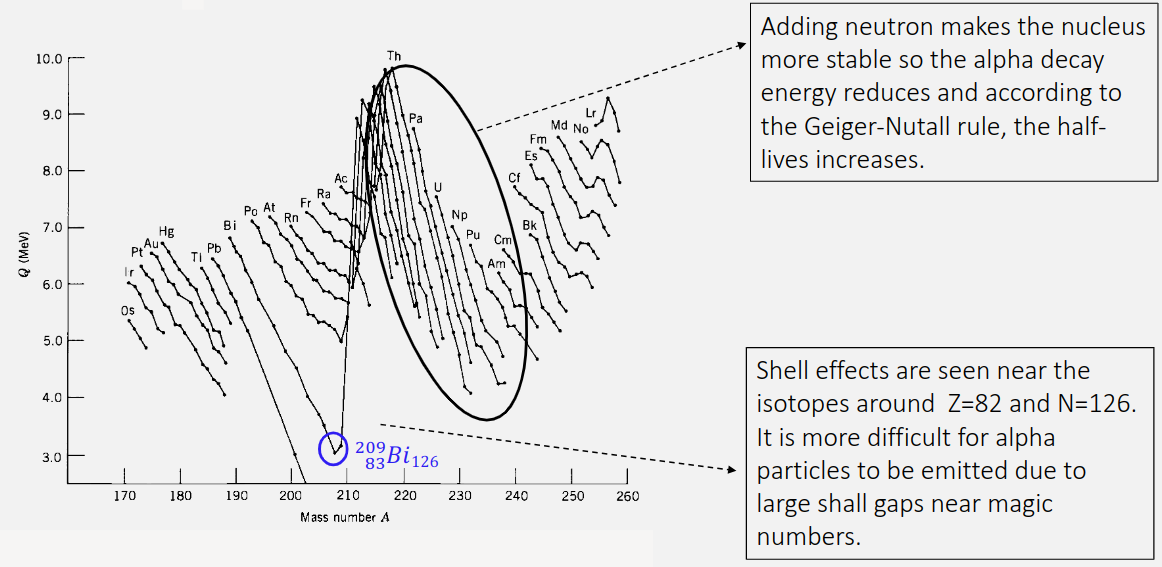
\includegraphics[width = .8\textwidth]{Q_v_A_systematics.png}
\caption{}
\label{fig: Q_v_A_systematics}
\end{figure}

\subsubsection{Theory of Alpha Decay}
\begin{itemize}
  \item Assuming the nucleus is full of alpha particles, we can calculate the probability of the alpha particle quantum tunneling through the potential barrier of the nucleus.
  \item We can view the regions as seen in \cref{fig: alpha_square_well} described classically or quantum mechanically.
\end{itemize}

\parbox[t]{\dimexpr\textwidth-\leftmargin}{%
\paragraph{Classical View}
\begin{wrapfigure}{r}{0.45\textwidth}
\vspace{3mm}
\centering
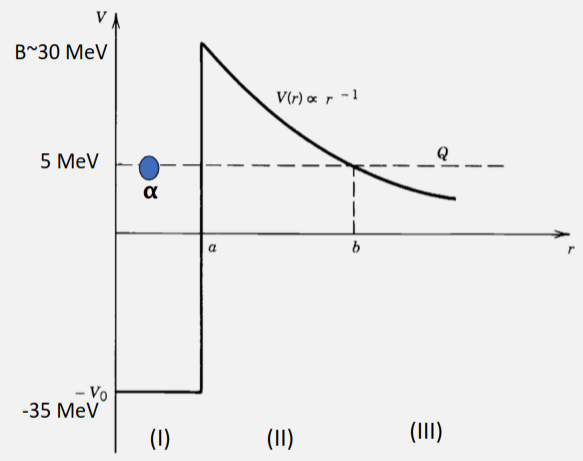
\includegraphics[width = .4\textwidth]{alpha_square_well.png}
\caption{Simple model of the nuclear potential creating a square well for the alpha particle. }
\label{fig: alpha_square_well}
\end{wrapfigure}
\begin{enumerate}[(I)]
  \item The alpha particle moves inside the potential well, but can't escape. 
  \item The region of the potential well. The alpha particle can't enter this region, as the potential is too high.
  \item Classically, the alpha particle is permitted to be on the outside, in this region, as the potential is lower than the energy of the alpha particle.
\end{enumerate}
\vspace{5mm}
}
  
  
\paragraph{Quantum Mechanical View}
\begin{itemize}
  \item The alpha particle will try to penetrate the potential barrier, and will make it after many attempts. 
  \item The barrier delays the emission. This is what gives the long half-life of alpha emitters. 
  \item The probability $λ$ of decay depends on frequency (how often the alpha particle tries to penetrate the barrier) and the probability of success. For alpha waves we have $λ = fP$. 
\end{itemize}

\paragraph{Example: $\ce{_{}^{235}\text{U}_{}}$}
\begin{itemize}
  \item We can calculate the barrier height $B$, by assuming we have an alpha particle stuck inside a thorium nucleus (as $\ce{_{92}^{235}\text{U}_{}} → \ce{_{90}^{231}\text{Th}_{}} + \ce{_{}^{4}\text{He}_{}}$). We inserting the number of protons in the Helium $Z_1$ and Thorium $Z_2$, and the radius of the two nuclei $R_1$ and $R_2$ into the formula. The radius is found by $R = R_0A^{1/3}$, where $R_0 = 1.2$ fm.
  \begin{equation}
    B = \frac{e^2}{4πϵ_0} \frac{Z_1 Z_2}{R_1 + R_2} = 1.44 \text{ MeV} ⋅  \text{fm} ⋅ \frac{2 ⋅ 90}{1.2 \left(4^{1/3} + 231^{1/3}\right)} ≈ 28 \text{ Mev}
  \end{equation}
  
  \item The Q-decay energy of the alpha particle is $4.6$ Mev. 

  \item The velocity of the alpha particle is found through the kinetic energy. The kinetic energy 
  \begin{equation}
    E_k = 5 + 35  = 40\text{ Mev} → v = 4.5 ⋅ 10^{7} \text{ m/s}
  \end{equation}
  \item The time it takes the particle to travel to the barrier can then be found:
  \begin{equation}
    t = R/v = \frac{7.5 ⋅ 10^{15}m}{4.5 ⋅ 10^{7}m/s} = 1.67 ⋅ 10^{-21}s
  \end{equation} 
  \item The frequency of the alpha particle trying to penetrate the barrier is then $f = 1/t = 6 ⋅ 10^{21}s^{-1}$.
  \item As the half-life of Uranium is around $10^9$, the alpha particle will attempt to penetrate the barrier $10^{41}$ times.
\end{itemize}

\subsubsection{Spin and Parity in Alpha Decay}
The total angular momentum carried by the alpha particle is only orbital, meaning $j_{α} = l_{α}$. The possible values of a final state $J_f$, from an initial state $J_i$ is given by $\left|J_i - J_f\right| ≤ l_{α} ≤ J_i + J_f$, with parity $π = (-1)^{l_α}$.

\paragraph{Example:}
\begin{wrapfigure}[9]{r}{0.5\textwidth}
\vspace{-5mm}
\centering
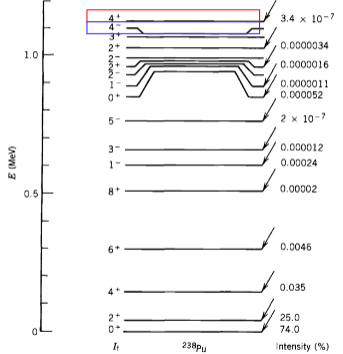
\includegraphics[width = .45\textwidth]{decay_intensity_by_state.png}
\caption{decay intensity of $\ce{_{}^{242}\text{Cm}_{}}$ to different excited states of $\ce{_{}^{238}\text{Pu}_{}}$. Blue: $4^{-}$-state, Red: $4^{+}$-state}
\label{fig: decay_intensity_by_state}
\end{wrapfigure}


Using the parity of each state as shown in \cref{fig: decay_intensity_by_state}, we can determine if a decay is allowed. As seen in blue, the $4^{-}$-state has $l_{α} = 4$, giving positive parity. This is conserved and therefore allowed. As seen in blue, we have the opposite, with non-conserved parity, which is therefore not allowed. 

If $l_{α}$ is even, the parity must be positive, and if $l_{α}$ is odd, the parity must be negative.

\vspace{40mm} %# 26
\section{Weak Interactions and Electroweak Unification: Continued}
\subsection{$Z^{0} / γ$ Interactions}
\begin{itemize}
    \item Any coupling to the photon $γ$ can in principle we written as a coupling to the $Z^{0}$ with a similar feynman diagram. Sometimes we must have separate diagrams for the two.
    \item We assume the boson couples with $u \bar{u}$, $c \bar{c}$, $t \bar{t}$, $d' \bar{d}'$, $s' \bar{s}'$ and $b' \bar{b}'$, as they couple to the charged interaction with the $W^{±}$-boson. 
    \item We go from the primed to the unprimed quarks trough the rotation matrix. We get the same result either way. 
    \begin{equation}
      d' \bar{d}' + s' \bar{s}' + b' \bar{b}' = \Big(V_{ij}(d, s, b)^{T}\Big)^{†} V_{ij}(\bar{d}, \bar{s}, \bar{b})^{T} = d \bar{d} + s \bar{s} + b \bar{b}
    \end{equation} 
    \item Both $γ$ and $Z^{0}$ are mixtures of $B^{0}$ and $W^{0}$, with $g' = g \tan θ_W$
\end{itemize}

\subsubsection{Electron-Antielectron to Neutrino-Antineutrino}
\begin{itemize}
    \item We have the cross section in for the photon and $Z^{0}$-boson:
    \begin{equation}
      σ_{γ} = α_{\text{EM}}^2(ℏc)^2 / E^2 \quad , \quad  σ_{Z} = G_{Z}^2 E^2 / (ℏc)^4
    \end{equation}
    \item At high energies where $E ≫ m_{Z}c^2$, we have: 
    \begin{equation}
      σ_{γ} / σ_{Z} ≈ 1 / \cos ^4 θ_{W} ≈ 1
    \end{equation}
    This is means they both have about equal contribution to the cross section. This is where we see unification. 
    \item At low energies where $E ≪ m_{Z}c^2$, we have:
    \begin{equation}
        σ_{γ}    / σ_{Z} ≈  \frac{1}{\cos ^4 θ_{W}} \frac{E^{4}}{M_{Z}^{4}} ≪ 1
    \end{equation}
    This is where the $Z^{0}$-boson contributes a lot more, and we have a clear difference between the forces with little unification. 
\end{itemize}

\subsection{BEH Mechanism}

\begin{itemize}
  \item Sometimes called the Higgs mechanism.
  \item To give the $W^{±}$ and $Z^{0}$ mass, we needed to break gauge symmetry. A way around this was found, by making the vacuum charged. This was done through a scalar field with non-zero value in the vacuum.
    \item The method was to create a Higgs field, with four components. The goal was to get three bosons with mass, and one without. 
    \item Three of the fields are absorbed by the $W^{±}$ and $Z^{0}$, giving them mass. This gives them 3 degrees of polarization, while the photon has 2.
    \item Exciting the fourth field gives the Higgs boson.
    \item This shows the vacuum is weakly charged. 
    \item Spontaneous symmetry breaking happens at low energies, as after being excited, the the fields falls down in a random direction. This happens even though the field is symmetric. This is visualized in \cref{fig: higgs_field}.    
\end{itemize}
\begin{figure}[ht!]
    \centering
    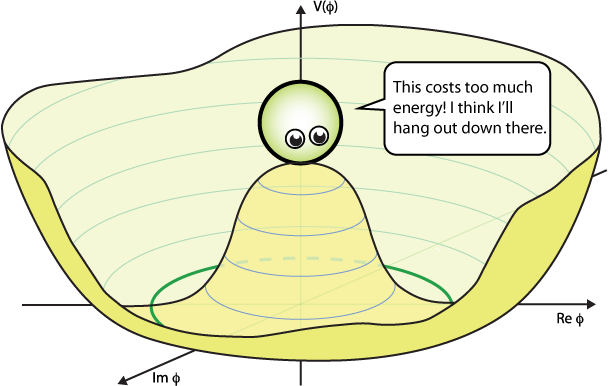
\includegraphics[width = .45\textwidth]{higgs_field.png}
    \caption{Visualization of the Higgs fields, when losing energy. After excitation, it falls down a random direction in the complex plane of the field. All directions have the same magnitude.}
    \label{fig: higgs_field}
\end{figure}

\subsubsection{Higgs Boson Decays}
\begin{itemize}
  \item Does not couple to color charges
  \item Can decay into a the top quark when its a virtual particle, with mass equal to the Higgs boson. Creating an top-antitop pair preserves color charge. This can also produce gluons. 
  \item While photons do not have mass, they can create leptons which later decay into photons.
  \item Some decay channels lead to four leptons. These are easy to detect and were seen as the golden path to finding the Higgs boson. The channel is very rare. 
  \item Some valid vertices are: 
  \begin{itemize}
    \item First order:
    \begin{align}
      &H → W^{+} W^{-} \\
      &H → Z^{0} Z^{0} \\
      &H → HH
    \end{align}
    \item Second order:
    \begin{align}
      &HH → W^{+} W^{-} \\
      &HH → Z^{0} Z^{0} \\
      &HH → HH
    \end{align}
  \end{itemize}
\end{itemize}

\subsubsection{Higgs Boson Experiment Summary}
\begin{itemize}
  \item The Higgs boson does not explain anything new, like dark matter etc. As dark matter have mass, the Higgs should help us understand it. 
  \item We have observe all proton-proton collisions. 
  \item We know it couples to vector bosons and 3rd generation fermions. The previous generations are not observed experimentally. 
  \item We have yet to observe the Higgs boson decaying into Higgs bosons.
\end{itemize} %# 27
\section{Symmetry: The Weak Interaction}
\subsection{Symmetry Breaking}
\begin{itemize}
    \item The breaking of gauge symmetry by the BEH mechanism is what gives mass. 
    \item Breaking of isospin symmetry by the $u$ and $d$ quark mass difference and electric charge difference. 
\end{itemize}
\subsubsection{Weak Parity Violation}
\paragraph{Cobalt Decay \cref{fig: cobalt_symmetry_breaking}}
Polarized $^{60}$Co decays into $^{60}$Ni, an electron neutrino and an electron. For parity to be conserved we would have\vbox{:}
\begin{wrapfigure}[8]{r}{0.45\textwidth}
\centering
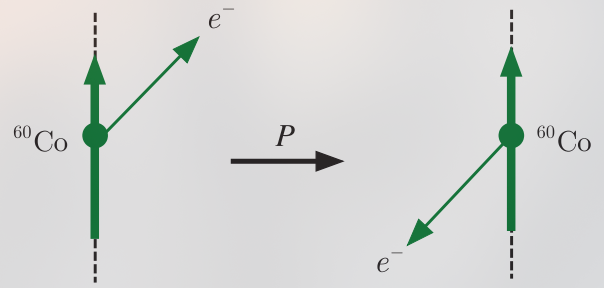
\includegraphics[width = .4\textwidth]{cobalt_symmetry_breaking.png}
\caption{Parity affecting the decay of a Cobalt atom.}
\label{fig: cobalt_symmetry_breaking}
\end{wrapfigure}
\begin{align}
  \vec{r} &→ -\vec{r} \\
  \vec{p} &→ -\vec{p} \\
  \vec{r} × \vec{p} &→ \vec{r} × \vec{p} \\
  \vec{J}, \vec{S}, \vec{L} &→ \vec{J}, \vec{S}, \vec{L}
\end{align}
This was experimentally shown to not be the case, as the above implies that there should be as many particles scattered at angle $θ$, as angel $π - θ$. 



\paragraph{Muon Decay \cref{fig: muon_symmetry_breaking}}
\begin{wrapfigure}[6]{r}{0.45\textwidth}
    \centering
    \vspace{-5mm}
    \includegraphics[width = .4\textwidth]{muon_symmetry_breaking.png}
    \caption{Parity affecting the decay of a muon.}
    \label{fig: muon_symmetry_breaking}
\end{wrapfigure}
\begin{itemize}
    \item We see parity not being conserved as $θ$ and $π - θ$ are not equal.
    \item We also see that $C$-parity is not conserved. 
    \item The product $CP$ is conserved, making the lifetime of $ℏ/Γ_{+} = ℏ/Γ_{-}$.     
\end{itemize}

\subsection{CP Conservation}
\begin{itemize}
  \item $CP$ is conserved when both $C$ and $P$ are conserved separately in the strong and electromagnetic interactions.
  \item $CP$ is conserved in nearly all weak interactions. 
\end{itemize}

\subsection{Chirality and Helicity}
\begin{itemize}
  \item Helicity is when the spin is in the same or opposite direction as the momentum. This can change for massless particles, as you can theoretically move faster than then, and from your perspective, the spin would be in the opposite direction.
  \item Chirality is harder to define, and represent an intrinsic property of a particle, as opposed to helicity being an observable which is relative. One can be left- or right-chiral. One can only change it by viewing it in a mirror image, as you flip it's spin, but not momentum. If you boost your velocity to be higher than a particle, it will change it's helicity, but not it's chirality.
  \item The weak interaction only couples to left-chiral particles and right-handed anti-particles, but both left and right-handed particles. 
\end{itemize}
\subsubsection{Right- and Left-Handedness \cref{fig: left_vs_right_handedness}}
\begin{figure}[h!]
\centering
\includegraphics[width = \textwidth]{left_vs_right_handedness.png}
\caption{Figure showing difference between left- and right-handed particles. A no-handed particle would have spin-0, or $J_z = 0$, meaning perpendicular to the direction of motion.}
\label{fig: left_vs_right_handedness}
\end{figure}

\subsubsection{The Weak Interaction}  
\begin{itemize}
  \item Eigenstates of the chirality takes part of the weak interaction as a conserved charge. 
  \item For massless particles, the helicity is the same as the chirality.
  \begin{equation}
    h ≡ \vec{J} ⋅  \frac{\vec{p}}{\left|\vec{p}\right|}
  \end{equation} 
  \item The helicity state's magnitude is the same as it's spin magnitude. The sign is positive for right-handed particles and negative for left-handed particles.
  \item Photons have only helicity $±1$, as they are massless.
  \item Massive bosons have helicity states $±1$ and $0$.
\end{itemize}


\subsubsection{Electron-Electron Scattering \cref{fig: electron_electron_parity}}
\begin{itemize}
  \item \textbf{Upper Left:} The initial beam is right-handed. 
  \item \textbf{Upper Right:} The beam becomes left-handed after the parity transformation. This is because both, momentum and position is flipped, but the spin is not.
  \item \textbf{Lower Right:} Changing our perspective by flipping $180^∘$ along the $y$-axis. 
  \item \textbf{Lower Left:} Changing our perspective by flipping $180^∘$ along the $x$-axis. We now have the original state, but with left-handed particles. For parity to be conserved, the cross section $σ_{R}$ and $σ_{L}$, should be the same, and they are. 
\end{itemize}
\begin{figure}[ht!]
\centering
\includegraphics[width = \textwidth]{electron_electron_parity.png}
\caption{Electron-electron scattering viewed from with after parity transformation and change of perspective.}
\label{fig: electron_electron_parity}
\end{figure}

\subsection{V - A Interaction}
\begin{itemize}
  \item $V$ is a vector interaction, like $\vec{r}$ changing sign under parity.
  \item $A$ is an axial vector interaction, like $\vec{L} ≡ \vec{r} × \vec{p}$ changing sign under parity.
  \item Both $\left|\mathcal{M}\right|^2 \propto \left|V^2\right|$ or $\left|A\right|^2$, would be parity conserving, but interference terms $\left|\mathcal{M}\right|^2 \propto \left|V - A\right|^2$ violates it. 
  \item $W^{±}$ couples to the $V-A$ weak current 
  \item $Z^{0}$ couples to mixtures of $V$ and $A$, depending on the 3rd component of weak isospin, electric charge and $\sin^2 θ_{W}$
\end{itemize}

\subsection{Neutral Kaon Oscillation}
\begin{itemize}
  \item The Kaon $d \bar{s}$, can oscillate between $K^{0}$ and $\bar{K}^{0}$. This is a $\left|ΔS\right| = 2$ transition allowed by second-order weak interactions. 
  \item It is second order because there are two decays, as seen in \cref{fig: kaon_oscillation}, and comes about because the decay products live long enough. 
\end{itemize}
\begin{figure}[h!]
\centering
\includegraphics[width = \textwidth]{kaon_oscillation.png}
\caption{Feynman diagram showing the oscillation of a neutral Kaon. $q$ can be any up-type quark, and $\bar{q}$ any up-type anti-quark.}
\label{fig: kaon_oscillation}
\end{figure}

 %# 28
\section{Beta Decay}
\begin{figure}[ht!]
\centering
\includegraphics[width = \textwidth]{radioactive_nuclei_chart.png}
\caption{Beta decay is most popular with smaller nuclei.}
\label{fig: radioactive_nuclei_chart_2}
\end{figure}

\subsection{$β^{-}$ Decay}
\vspace{1mm}
\begin{wrapfigure}[7]{r}{0.45\textwidth}
\centering
\vspace{-12.5mm}
\includegraphics[width = .35\textwidth]{beta_minus_decay.png}
\caption{Feynman diagram of $β^{-}$ decay.}
\label{fig: beta_minus_decay}
\end{wrapfigure}
The neutron turns into a proton, electron and electron anti-neutrino. Only the electron and anti-neutrino are emitted. 
\begin{equation}
    n \rightarrow p + e^{-} + \bar{\nu}_{e} + Q_β
\end{equation}
This comes from the down quark turning into an up quark as seen in \cref{fig: beta_minus_decay}.



\vspace{12mm}
\subsection{$β^{+}$ Decay}
\begin{wrapfigure}[7]{r}{0.45\textwidth}
\centering
\vspace{-10mm}
\includegraphics[width = .35\textwidth]{beta_plus_decay.png}
\caption{Feynman diagram of $β^{+}$ decay.}
\label{fig: beta_plus_decay}
\end{wrapfigure}
The proton turns into a neutron, positron and electron neutrino. Only the positron and neutrino are emitted.
\begin{equation}
    p \rightarrow n + e^{+} + \nu_{e} + Q_β
\end{equation}
This comes from the up quark turning into a down quark as seen in \cref{fig: beta_plus_decay}.


\vspace{10mm}
\subsection{Electron Capture}
\begin{wrapfigure}[13]{r}{0.45\textwidth}
\centering
\includegraphics[width = .35\textwidth]{electron_capture.png}
\caption{Feynman diagram of electron capture.}
\label{fig: electron_capture}
\end{wrapfigure}

The nucleus captures an electron and turns a proton and electron into a neutron and electron neutrino. 
\begin{equation}
    p + e^{-} \rightarrow n + \nu_{e} + Q_β
\end{equation}
This comes from the up quark turning into a down quark. Only the neutrino is emitted as seen in \cref{fig: electron_capture}.

\vspace{10mm}
\subsection{Free Proton Decay}
\begin{itemize}
    \item A free proton can not decay. It will only decay inside the nucleus because of the binding energy, through beta decay and electron capture. 
    \item When decaying, the mass of the entire system is reduced. This cannot happen for a lone proton. 
\end{itemize}

\subsection{Energy Conservation}
\subsubsection{Neutron Decay}

We assume the neutron is at rest before the decay. 
\begin{equation}
    m_nc^2 = m_pc^2 + m_ec^2 + m_{\bar{\nu}_e}c^2 + K_{e} + K_{p} + K_{\bar{ν}}
\end{equation}
We define the $Q$-value:
\begin{equation}
    Q = \left(m_n - m_p - m_e - m_{\bar{ν}}\right)c^2
\end{equation}
Inserting the $Q$-value into the energy conservation equation:
\begin{equation}
    Q = K_{e} + K_{p} + K_{\bar{ν}}
\end{equation}
The recoil experienced by the proton is so small, as is the mass of the anti-neutrino. We tend to ignore both, giving:
\begin{equation}
    Q = m_n - m_p - m_e ≈ K_{e} + K_{\bar{ν}}
\end{equation}


\subsubsection{$β^{-}$ Decay}
We now consider the nucleus at rest before the decay.
\begin{equation}
  \ce{_{Z}^{A}\text{X}_{N}} → \ce{_{Z+1}^{A}\text{Y}_{N-1}} + e^{-} + \bar{\nu}_{e}
\end{equation}
The $Q$-value is derived from the nuclear mass $m_{N}$. We ignore the mass of the anti-neutrino. Nuclear masses is defined as follows:
\begin{equation}
  m\left(\ce{_{}^{A}\text{X}_{}}\right)c^2 = m_{N}\left(\ce{_{}^{A}\text{X}_{}}\right)c^2 + Zm_e c^2 - ∑_{i=1}^{Z} B_i
\end{equation}
\begin{equation}
  Q_{β^{-}} = \Big(m_{N} \left(\ce{_{Z}^{A}\text{X}_{}}\right) - m_{N}\left(\ce{_{Z+1}^{A}\text{Y}_{}}\right) - m_e\Big)c^2
\end{equation}
Adding the definition of the nuclear mass:
\begin{equation}
    Q_{β^{-}} = \Bigg[\Big(M\left(\ce{_{}^{A}\text{X}_{}}\right) - Zm_e\Big)- \bigg(m\Big(\ce{_{}^{A}\text{Y}_{}}\Big) - (Z+1)m_e\bigg) - m_e\Bigg]c^2 + ∑_{i=1}^{Z} B_i - ∑_{i=1}^{Z + 1} B_i
\end{equation}
Ignoring the binding energy of the electrons, we get:
\begin{equation}
  Q_{β^{-}} = \Big(m\left(\ce{_{}^{A}\text{X}_{}}\right) - m\left(\ce{_{}^{A}\text{Y}_{}}\right)\Big)c^2
\end{equation}

\paragraph{Example:}
Decay of $\ce{_{}^{210}\text{Bi}_{}}$ into $\ce{_{}^{210}\text{Po}_{}} + e + \bar{ν}_e$:
\begin{equation}
  Q_{β^{-}} = \Big(m\left(\ce{_{}^{210}\text{Bi}_{}}\right) - m\left(\ce{_{}^{210}\text{Po}_{}}\right)\Big)c^2 = 1.16 \text{ MeV}
\end{equation}
This sets an upper limit for the possible kinetic energy of the electron, and the energy of the anti-neutrino.
\begin{equation}
  K_{e_{\text{max}}} = E_{p_{\text{max}}} = Q_{β^{-}} = 1.16 \text{ MeV}
\end{equation}

\subsubsection{Electron Capture}
\begin{equation}
    \ce{_{Z}^{A}\text{X}_{N}} + e^{-} → \ce{_{Z-1}^{A}\text{Y}_{N+1}} + \nu_{e}
\end{equation}
\begin{equation}
  Q_{ε} = \Big(m\left(\ce{_{}^{A}\text{X}_{}}\right) - m\left(\ce{_{}^{A}\text{Y}_{}}\right)\Big)c^2 - B_n
\end{equation}
Where $B_n$ is the electron binding energy, depending on shell number $n$. Using conservation of energy we get:
\begin{equation}
    Q_{ε} = K_{\ce{_{}^{A}\text{Y}_{}}} + K_{\nu} ≈ K_{ν}
\end{equation}

This is a two-body decay, so the expected energy distribution is very sharp. As opposed to the three-body decay of $β^{-}$ decay, with a continuous energy distribution, as seen in \cref{fig: electron_energy_distribution}.

\begin{figure}[h!]
\centering
\includegraphics[width = .6\textwidth]{electron_energy_distribution.png}
\caption{Expected energy distribution for electrons in two-body and three-body decays.}
\label{fig: electron_energy_distribution}
\end{figure}

\subsubsection{Comparing Electron Capture \& $β^{+}$ Decay}
We have the $Q$-values for both processes:
\begin{equation}
    Q_{ε} = \Big(m\left(\ce{_{}^{A}\text{X}_{}}\right) - m\left(\ce{_{}^{A}\text{Y}_{}}\right)\Big)c^2 - B_n \quad , \quad  Q_{β^{+}} = \Big(m\left(\ce{_{}^{A}\text{X}_{}}\right) - m\left(\ce{_{}^{A}\text{Y}_{}}\right) - 2m_e\Big)c^2
\end{equation}
As $B_n ≪ 2m_ec^2$, we know that if a nucleus is able to undergo $β^{+}$ decay, has the energy to undergo electron capture. The opposite is not necessarily true. To undergo spontaneous $β^{+}$ decay, the $Q$-value must be equal or greater than $2m_ec^2 ≈ 1$ MeV. \\

The larger the $Q$-value the shorter the half-life. This is because the decay is more likely to happen if the energy released is higher.

\subsection{Fermi's Golden Rule}    
The decay probability $λ$ is constant and is given by:
\begin{equation}
  λ = \frac{1}{τ} = \frac{2π}{ℏ} |V_{fi}|^2 ρ(E_f)  \quad , \quad  V_{fi} = ∫ ψ^{*}_f V ψ_i dν
\end{equation}

\vspace{15mm}
It depends on: 
\begin{itemize}
    \item The density of the final state which decay can proceed. The higher the density, the faster the decay. 
    \item The matrix element describes the strength of the interaction, both strong and weak. 
    \item It Describes the overlap between the wave functions of initial and final states. The larger the overlap, the faster the decay occurs. 
\end{itemize}

\subsubsection{Fermi's Golden Rule for Decay}
These were points Fermi's theory had to address. 
\paragraph{Beta Decay:}
\begin{enumerate}
    \item Electron and neutrino do not exist before the decay process. The theory must account for their formation.
    \item Electron and neutrino must be treated relativistically. 
    \item The continuous distribution of electron energies must be reproduced by the theory (three body).
\end{enumerate}

\paragraph{Alpha Decay:}
\begin{enumerate}
    \item Alpha particle existed before the decay. 
    \item Alpha particle is treated classically.
    \item Alpha particle energy distributions monoenergetic (two body).
\end{enumerate}

\subsubsection{Fermi's Theory of Beta Decay}
Fermi introduced a small pertubation $V'$ to the state of the nucleus. This would have to be a weak interaction, compared to the strong interaction. This would explain why the decay is slow (seconds and longer), compared to the fast strong interaction.  %# 29
\section{Symmetry Breaking Weak Interactions}
\subsection{Key Questions About CP-Violation}   
\begin{itemize}
    \item Is the $CP$-violation in the $K^{0}$ system due to mixing or direct violation?
    \item \textbf{Mixing:} The $K^{0}_{S}$ and $K^{0}_{L}$ are non-orthogonal mixtures of $CP$-eigenstates. 
    \begin{equation}
      \ket{K^{0}_{S}, 0} = \frac{1}{\sqrt{1 + \left|ϵ\right|^2}} \left(\ket{K_1^{0}, 0} + \ket{K_2^{0}, 0}\right)
    \end{equation}
    \begin{equation}
        \ket{K^{0}_{L}, 0} = \frac{1}{\sqrt{1 + \left|ϵ\right|^2}} \left(ϵ\ket{K_1^{0}, 0} - \ket{K_2^{0}, 0}\right)
    \end{equation}
    \textbf{Direct:} The $K^{0}_{S}$ and $K^{0}_{L}$ are pure $CP$-eigenstates. Decaying to forbidden $CP$-states. 
    \begin{equation}
        \ket{K^{0}_{S}, 0} = \ket{K_1^{0}, 0}
    \end{equation}
    \begin{equation}
        \ket{K^{0}_{L}, 0} = \ket{K_2^{0}, 0}
    \end{equation} 
    \item \textbf{Conclusion:} There is both mixing and direct violation. The mixing is the dominant part. 
\end{itemize}













\subsubsection{CPT Invariance}
\begin{itemize}
    \item Predicted to be conserved in quantum field theory. If you break $CP$, you must also break $T$, meaning time. 
    \item This predicts the mass of particles and anti-particles should be the same. 
    \item There is yet to be found an exception to $CPT$-invariance. 
\end{itemize}


\subsection{CP and Flavour Oscillations in B-Decays}
\begin{itemize}
    \item Direct $CP$-violation plays a much larger role in $B$-decays than in $K$-decays.
    \item We have mixing, direct breaking, and interference. 
    \item We see this in both charged and neutral $B$-decays, but not for mixing. This is because the mixing requires charged to be conserved. 
\end{itemize}

\subsection{Wolfenstein Parametrization}
\begin{itemize}
    \item A first order parametrization of the CKM-matrix.
    \begin{equation}
        V_{\text{WP}} = \begin{pmatrix}
            1 - \frac{1}{2}λ^2 - \frac{λ^{4}}{8} & λ & Aλ^3(\rho - iη) \\
            -λ + A^2λ^{5} \left(1 - 2 (ρ + iη)\right) / 2 & 1 - \frac{1}{2}λ^2 & Aλ^2 \\
            Aλ^3(1 - (1 - λ)(ρ + iη)) & -Aλ^2 + Aλ^{4}(1 - 2(ρ + i η)) / 2 & 1 - A^2λ^4 / 2
        \end{pmatrix}
    \end{equation}
    \item It tells us that $CP$-violation is small in strange and charm sectors, which are dominated by mixing. 
    \item The bottom section have a large $CP$-violation. 
    \item The top quark it is predicted to have a small $CP$-violation. If this is found, it would be a strong indication of new physics.
\end{itemize}
 %# 30
\input{W18-1} %# 31
\input{W18-2} %# 32
\input{W19-1} %# 33
\input{W19-2} %# 34
\input{W20-1} %# 35
\input{W20-2} %# 36
\input{W21-1} %# 37
\input{W21-2} %# 38


\end{document}